%!TEX TS-program = pdflatex
%!TEX encoding = UTF-8 Unicode
%!BIB program = bibtex

\PassOptionsToPackage{usenames,dvipsnames,table}{xcolor}
\documentclass{mimosis}
% \documentclass[draft]{mimosis}


\usepackage{metalogo}

%%%%%%%%%%%%%%%%%%%%%%%%%%%%%%%%%%%%%%%%%%%%%%%%%%%%%%%%%%%%%%%%%%%%%%%%
% Some of my favourite personal adjustments
%%%%%%%%%%%%%%%%%%%%%%%%%%%%%%%%%%%%%%%%%%%%%%%%%%%%%%%%%%%%%%%%%%%%%%%%
%
% These are the adjustments that I consider necessary for typesetting
% a nice thesis. However, they are *not* included in the template, as
% I do not want to force you to use them.

% This ensures that I am able to typeset bold font in table while still aligning the numbers
% correctly.
\usepackage{etoolbox}

\usepackage{siunitx}
\DeclareSIUnit\px{px}

\sisetup{%
  detect-all           = true,
  detect-family        = true,
  detect-mode          = true,
  detect-shape         = true,
  detect-weight        = true,
}

%%%%%%%%%%%%%%%%%%%%%%%%%%%%%%%%%%%%%%%%%%%%%%%%%%%%%%%%%%%%%%%%%%%%%%%%
% Hyperlinks & bookmarks
%%%%%%%%%%%%%%%%%%%%%%%%%%%%%%%%%%%%%%%%%%%%%%%%%%%%%%%%%%%%%%%%%%%%%%%%

\def\oubli#1{}


\usepackage[%
  unicode,
  colorlinks = true,
  citecolor  = RoyalBlue,
  linkcolor  = RoyalBlue,
  urlcolor   = RoyalBlue,
  unicode,
  ]{hyperref}
\hypersetup{
  pdftitle=Public-Data Pretraining for Clinical Information Extraction,
  pdfauthor=Rian Touchent,
}

\usepackage{bookmark}

%%%%%%%%%%%%%%%%%%%%%%%%%%%%%%%%%%%%%%%%%%%%%%%%%%%%%%%%%%%%%%%%%%%%%%%%
% Fonts
%%%%%%%%%%%%%%%%%%%%%%%%%%%%%%%%%%%%%%%%%%%%%%%%%%%%%%%%%%%%%%%%%%%%%%%%

\ifxetexorluatex
  \setmainfont[Ligatures=TeX]{TeX Gyre Pagella} % Palatino clone
  \linespread{1.05} % a bit more for Palatino
  \RequirePackage{unicode-math}
  \setmathfont{TeX Gyre Pagella Math}
\else
  \usepackage[lf]{ebgaramond}
  \usepackage[oldstyle,scale=0.7]{sourcecodepro}
  \singlespacing
\fi

\usepackage{microtype}

\renewcommand{\th}{\textsuperscript{\textup{th}}\xspace}

% =====================================================================
% Acronyms and glossary.
% \input before \makeglossaries in thesis.tex.
% Acronyms = factual expansions of abbreviations (no sourced definition).
% Glossary entries = concepts with a definition taken from a recognized,
% cited authoritative reference (never invented). See sources/ research notes.
% Model names (CamemBERT, BERT, GPT, ...) are proper nouns introduced and
% cited in the text, so they are deliberately NOT listed as acronyms.
% =====================================================================

% ---------------------------------------------------------------------
% Acronyms
% ---------------------------------------------------------------------

% General machine learning / NLP
\newacronym{AI}{AI}{artificial intelligence}
\newacronym{NLP}{NLP}{natural language processing}
\newacronym{LLM}{LLM}{large language model}
\newacronym{MLM}{MLM}{masked language modeling}
\newacronym{CLM}{CLM}{causal language modeling}
\newacronym{NER}{NER}{named entity recognition}
\newacronym{IE}{IE}{information extraction}
\newacronym{QA}{QA}{question answering}
\newacronym{CPT}{CPT}{continued pretraining}
\newacronym{DAPT}{DAPT}{domain-adaptive pretraining}
\newacronym{TAPT}{TAPT}{task-adaptive pretraining}
\newacronym{RoPE}{RoPE}{rotary position embedding}
\newacronym{BPE}{BPE}{byte-pair encoding}
\newacronym{CKA}{CKA}{centered kernel alignment}
\newacronym{MAP}{MAP}{mean average precision}
\newacronym{MMLU}{MMLU}{Massive Multitask Language Understanding}
\newacronym{GPU}{GPU}{graphics processing unit}
\newacronym{RDF}{RDF}{Resource Description Framework}
\newacronym{JSON}{JSON}{JavaScript Object Notation}

% Biomedical / clinical
\newacronym{PMC}{PMC}{PubMed Central}
\newacronym{UMLS}{UMLS}{Unified Medical Language System}
\newacronym{MeSH}{MeSH}{Medical Subject Headings}
\newacronym{SNOMEDCT}{SNOMED CT}{Systematized Nomenclature of Medicine Clinical Terms}
\newacronym{ICD}{ICD}{International Classification of Diseases}
\newacronym{CIM}{CIM-10}{Classification internationale des maladies, 10\textsuperscript{e} révision}
\newacronym{CCAM}{CCAM}{Classification commune des actes médicaux}
\newacronym{ATC}{ATC}{Anatomical Therapeutic Chemical classification}
\newacronym{PMSI}{PMSI}{Programme de médicalisation des systèmes d'information}
\newacronym{EHR}{EHR}{electronic health record}
\newacronym{CDW}{CDW}{clinical data warehouse}
\newacronym{RCP}{RCP}{réunion de concertation pluridisciplinaire}

% Neural architectures and training (added from completeness sweep)
\newacronym{RNN}{RNN}{recurrent neural network}
\newacronym{LSTM}{LSTM}{long short-term memory}
\newacronym{BiLSTM}{BiLSTM}{bidirectional long short-term memory}
\newacronym{GRU}{GRU}{gated recurrent unit}
\newacronym{CRF}{CRF}{conditional random field}
\newacronym{GLU}{GLU}{gated linear unit}
\newacronym{RMSNorm}{RMSNorm}{root mean square normalization}
\newacronym{ALiBi}{ALiBi}{attention with linear biases}
\newacronym{GQA}{GQA}{grouped-query attention}
\newacronym{RLHF}{RLHF}{reinforcement learning from human feedback}
\newacronym{RLVR}{RLVR}{reinforcement learning with verifiable rewards}
\newacronym{GRPO}{GRPO}{group relative policy optimization}
\newacronym{FP8}{FP8}{8-bit floating point}
\newacronym{MSE}{MSE}{mean squared error}
\newacronym{MAE}{MAE}{mean absolute error}
\newacronym{IOB2}{IOB2}{inside--outside--beginning tagging scheme}

% Formats, standards, semantic web
\newacronym{XML}{XML}{Extensible Markup Language}
\newacronym{OCR}{OCR}{optical character recognition}
\newacronym{OWL}{OWL}{Web Ontology Language}
\newacronym{SKOS}{SKOS}{Simple Knowledge Organization System}
\newacronym{W3C}{W3C}{World Wide Web Consortium}

% Document structures
\newacronym{IMRAD}{IMRAD}{introduction, methods, results, and discussion}
\newacronym{SOAP}{SOAP}{subjective, objective, assessment, plan}

% Organisations and regulations
\newacronym{WHO}{WHO}{World Health Organization}
\newacronym{NCBI}{NCBI}{National Center for Biotechnology Information}
\newacronym{EMA}{EMEA}{European Medicines Agency}
\newacronym{ATIH}{ATIH}{Agence technique de l'information sur l'hospitalisation}
\newacronym{SMT}{SMT}{serveur multi-terminologies}
\newacronym{CNIL}{CNIL}{Commission nationale de l'informatique et des libertés}
\newacronym{HIPAA}{HIPAA}{Health Insurance Portability and Accountability Act}

% ---------------------------------------------------------------------
% Glossary entries (definitions sourced from cited authoritative references)
% Kept only terms present in the body (grep-verified); definitions never
% invented. See research/glossary_mlnlp.md and research/glossary_clinical.md.
% ---------------------------------------------------------------------

% --- Machine learning / NLP concepts ---
\newglossaryentry{language-model}{name={language model}, description={A model that predicts upcoming words, assigning a probability to each possible next word and thereby to an entire word sequence~\citep{jurafsky_course}.}, sort={language model}}
\newglossaryentry{n-gram-language-model}{name={n-gram language model}, description={A language model that approximates the probability of a word given its full history by conditioning only on the previous $n-1$ words, following the Markov assumption that the recent context suffices~\citep{jurafsky_course}.}, sort={n-gram language model}}
\newglossaryentry{masked-language-modeling}{name={masked language modeling}, description={A pretraining objective in which a random subset of input tokens is replaced by a mask symbol and the model is trained to recover the original tokens from their bidirectional context~\citep{devlin_bert_2019}.}, sort={masked language modeling}}
\newglossaryentry{causal-language-modeling}{name={causal (autoregressive) language modeling}, description={A training objective in which the model predicts each token conditioned only on the preceding tokens, factorising the sequence probability left to right via the chain rule of probability~\citep{jurafsky_course}.}, sort={causal language modeling}}
\newglossaryentry{pretraining}{name={pretraining}, description={Training a model on one task or dataset so that its learned representations can initialise and improve learning on a different, typically downstream, task~\citep{goodfellow_deep_2016}.}, sort={pretraining}}
\newglossaryentry{fine-tuning}{name={fine-tuning}, description={Adapting a pretrained model to a target task by continuing training, usually with supervised data, so that its general representations are specialised to that task~\citep{devlin_bert_2019}.}, sort={fine-tuning}}
\newglossaryentry{continual-pretraining}{name={continued pretraining (domain-adaptive pretraining)}, description={A second phase of self-supervised pretraining of an already pretrained language model on unlabelled in-domain text, which improves downstream performance within that domain~\citep{gururangan_dont_2020}.}, sort={continued pretraining}}
\newglossaryentry{transformer}{name={transformer}, description={A sequence-transduction architecture that replaces recurrence and convolution entirely with stacked self-attention and position-wise feed-forward layers~\citep{vaswani2017attention}.}, sort={transformer}}
\newglossaryentry{attention}{name={attention}, description={A mechanism that computes an output as a weighted sum of value vectors, where each weight is given by a compatibility function between a query and the corresponding key~\citep{vaswani2017attention}.}, sort={attention}}
\newglossaryentry{self-attention}{name={self-attention}, description={An attention mechanism in which the queries, keys, and values are all derived from the same sequence, relating different positions of that sequence to compute its representation~\citep{vaswani2017attention}.}, sort={self-attention}}
\newglossaryentry{encoder-decoder}{name={encoder and decoder architecture}, description={A model design in which an encoder maps an input sequence to a sequence of continuous representations and a decoder then generates the output sequence one element at a time from those representations~\citep{vaswani2017attention}.}, sort={encoder and decoder architecture}}
\newglossaryentry{tokenization}{name={tokenization}, description={The process of segmenting a running text into the discrete tokens that serve as the model's atomic input units~\citep{jurafsky_course}.}, sort={tokenization}}
\newglossaryentry{subword-tokenization}{name={subword tokenization}, description={A tokenization strategy that represents words as sequences of frequent subword units, learned for example by iteratively merging the most frequent adjacent symbol pairs as in byte-pair encoding~\citep{sennrich-etal-2016-neural}.}, sort={subword tokenization}}
\newglossaryentry{perplexity}{name={perplexity}, description={An intrinsic evaluation measure for language models equal to the inverse probability of a test set normalised by the number of words, so that a lower value indicates a better model~\citep{jurafsky_course}.}, sort={perplexity}}
\newglossaryentry{named-entity-recognition}{name={named entity recognition}, description={The task of finding spans of text that constitute proper names and classifying each into a predefined entity type such as person, location, or organisation~\citep{jurafsky_course}.}, sort={named entity recognition}}
\newglossaryentry{information-extraction}{name={information extraction}, description={The process of turning unstructured text into structured data, for example by recognising entities and the relations that hold among them~\citep{jurafsky_course}.}, sort={information extraction}}
\newglossaryentry{knowledge-distillation}{name={knowledge distillation}, description={A model-compression technique in which a small student model is trained to reproduce the output distribution of a larger teacher model, transferring its knowledge into a more compact form~\citep{sanh2019distilbert}.}, sort={knowledge distillation}}
\newglossaryentry{contrastive-learning}{name={contrastive learning}, description={A representation-learning approach that pulls representations of matched (positive) pairs together while pushing apart those of unmatched (negative) pairs~\citep{gao-etal-2021-simcse}.}, sort={contrastive learning}}
\newglossaryentry{in-context-learning}{name={zero-shot, few-shot, and in-context learning}, description={The ability of a large language model to perform a new task at inference time from a natural-language description alone (zero-shot) or from a few demonstrations placed in its prompt (few-shot), without any gradient updates~\citep{gpt3}.}, sort={zero-shot, few-shot, and in-context learning}}
\newglossaryentry{rope}{name={rotary position embedding (RoPE)}, description={A position-encoding scheme that injects positional information by rotating the query and key vectors by an angle proportional to their absolute position, so that their dot product depends only on the relative distance between tokens~\citep{rope}.}, sort={rotary position embedding}}
\newglossaryentry{cross-entropy-loss}{name={cross-entropy loss}, description={A training objective equal to the negative log-likelihood of the data under the model, measuring the dissimilarity between the model's predicted distribution and the empirical target distribution~\citep{goodfellow_deep_2016}.}, sort={cross-entropy loss}}
\newglossaryentry{mean-average-precision}{name={mean average precision}, description={The mean over a set of queries of the average precision, where average precision is the mean of the precision values computed at each rank position at which a relevant item is retrieved~\citep{manning_ir_2008}.}, sort={mean average precision}}
\newglossaryentry{f1-score}{name={F1 score}, description={The harmonic mean of precision and recall, summarising both in a single value that gives equal weight to the two~\citep{jurafsky_course}.}, sort={F1 score}}

% --- Clinical / biomedical concepts ---
\newglossaryentry{clinical-case-report}{name={clinical case report}, description={A detailed narrative describing the diagnosis, treatment and follow-up of an individual patient, used in French clinical NLP as a publicly shareable proxy for hospital notes~\citep{grouin_clinical_2019}.}, sort={clinical case report}}
\newglossaryentry{ehr}{name={electronic health record (EHR)}, description={A digital, longitudinal collection of a patient's health information recorded during care, comprising structured data and free-text clinical notes~\citep{aphp_cdw}.}, sort={electronic health record}}
\newglossaryentry{cdw}{name={clinical data warehouse (CDW)}, description={A hospital database that aggregates and integrates clinical data from operational care systems for secondary use such as research and decision support~\citep{aphp_cdw}.}, sort={clinical data warehouse}}
\newglossaryentry{de-identification}{name={de-identification}, description={The task of detecting and removing or replacing protected health information, such as names, dates and locations, from clinical text so that patients cannot be identified~\citep{stubbs_deid_2015}.}, sort={de-identification}}
\newglossaryentry{pseudonymisation}{name={pseudonymisation}, description={Under the GDPR, the processing of personal data so that it can no longer be attributed to a specific data subject without separately kept additional information, meaning the data remains personal data~\citep{gdpr_art4}.}, sort={pseudonymisation}}
\newglossaryentry{clinical-information-extraction}{name={clinical information extraction}, description={The natural language processing task of automatically extracting structured information, such as medical concepts, assertions and relations, from free-text clinical narratives~\citep{neveol_clinical_2016}.}, sort={clinical information extraction}}
\newglossaryentry{medical-coding}{name={medical coding}, description={The assignment of standardised codes from a controlled classification, such as ICD or CCAM, to the diagnoses and procedures recorded in a patient's clinical documentation~\citep{atih_pmsi}.}, sort={medical coding}}
\newglossaryentry{umls}{name={Unified Medical Language System (UMLS)}, description={A set of files and software produced by the U.S. National Library of Medicine that brings together many health and biomedical vocabularies to enable interoperability between computer systems~\citep{bodenreider_unified_2004}.}, sort={Unified Medical Language System}}
\newglossaryentry{snomed-ct}{name={SNOMED CT}, description={The comprehensive, multilingual clinical healthcare terminology maintained by SNOMED International, designed for the consistent representation of clinical content in electronic health records~\citep{snomed_ct}.}, sort={SNOMED CT}}
\newglossaryentry{icd-10}{name={ICD-10}, description={The tenth revision of the World Health Organization's International Statistical Classification of Diseases and Related Health Problems, the global standard for recording and comparing diagnoses~\citep{who_icd10}.}, sort={ICD-10}}
\newglossaryentry{cim-10-pmsi}{name={CIM-10 (PMSI)}, description={The French-language version of the WHO International Classification of Diseases (tenth revision), maintained by the ATIH and used since 1996 to code diagnoses in the standardised records of the PMSI~\citep{atih_cim10}.}, sort={CIM-10 (PMSI)}}
\newglossaryentry{ccam}{name={CCAM}, description={The Classification commune des actes médicaux, the French national classification used since 2004 to code the medical and technical procedures performed by physicians~\citep{atih_ccam}.}, sort={CCAM}}
\newglossaryentry{atc}{name={ATC classification}, description={The Anatomical Therapeutic Chemical classification maintained by the WHO Collaborating Centre for Drug Statistics Methodology, which classifies active substances into five hierarchical levels by the organ or system they act on and their therapeutic and chemical properties~\citep{whocc_atc}.}, sort={ATC classification}}
\newglossaryentry{pmsi}{name={PMSI}, description={The Programme de médicalisation des systèmes d'information, the French scheme that produces a standardised synthetic description of hospital medical activity from systematically recorded medico-administrative data~\citep{atih_pmsi}.}, sort={PMSI}}
\newglossaryentry{mesh}{name={MeSH}, description={Medical Subject Headings, a controlled and hierarchically organised vocabulary produced by the U.S. National Library of Medicine for indexing, cataloguing and searching biomedical information~\citep{nlm_mesh}.}, sort={MeSH}}
\newglossaryentry{rcp}{name={réunion de concertation pluridisciplinaire (RCP)}, description={A meeting between health professionals, mandatory in French cancer care, at which a patient's situation and the possible treatments are discussed in light of current scientific evidence and their benefits and risks~\citep{inca_rcp}.}, sort={reunion de concertation pluridisciplinaire}}

% --- Concepts added from the completeness sweep ---
\newglossaryentry{knowledge-graph}{name={knowledge graph}, description={A graph of data intended to accumulate and convey knowledge of the real world, whose nodes represent entities of interest and whose edges represent relations between these entities~\citep{hogan_knowledge_2021}.}, sort={knowledge graph}}
\newglossaryentry{ontology}{name={ontology}, description={An explicit specification of a conceptualisation, that is, of the objects, concepts, and relations assumed to exist in some area of interest and the relationships that hold among them~\citep{gruber_ontology_1993}.}, sort={ontology}}
\newglossaryentry{entity-linking}{name={entity linking}, description={The task of linking a named-entity mention in text to its corresponding entry in a reference knowledge base, resolving the mention to the real-world entity it denotes~\citep{shen_entity_2015}.}, sort={entity linking}}
\newglossaryentry{sequence-labeling}{name={sequence labeling}, description={The task of assigning a label to each element of an input sequence, modelled jointly over the whole sequence so that the prediction for one position depends on neighbouring labels~\citep{lafferty2001crf}.}, sort={sequence labeling}}
\newglossaryentry{multi-label-classification}{name={multi-label classification}, description={A classification task in which each instance may be associated with a set of several labels at once, rather than with a single mutually exclusive class~\citep{tsoumakas_multilabel_2007}.}, sort={multi-label classification}}
\newglossaryentry{nested-entities}{name={nested entities}, description={In named entity recognition, entity mentions that contain other entity mentions within their span, so that a single token can belong to more than one entity at once~\citep{finkel_nested_2009}.}, sort={nested entities}}
\newglossaryentry{catastrophic-forgetting}{name={catastrophic forgetting}, description={The tendency of a connectionist network to abruptly lose previously learned knowledge when it is trained on new information~\citep{mccloskey1989catastrophic}.}, sort={catastrophic forgetting}}
\newglossaryentry{scaling-laws}{name={scaling laws}, description={Empirical power-law relationships showing that the cross-entropy loss of a language model decreases predictably with model size, dataset size, and training compute~\citep{kaplan_scaling}.}, sort={scaling laws}}
\newglossaryentry{benchmark-contamination}{name={benchmark contamination}, description={The situation in which test or benchmark data has leaked into a model's training corpus, so that evaluation scores reflect memorisation rather than genuine generalisation~\citep{xu2024contaminationsurvey}.}, sort={benchmark contamination}}
\newglossaryentry{micro-macro-averaging}{name={micro- and macro-averaging}, description={Two ways of aggregating a per-class measure such as precision, recall, or F1 over several classes: micro-averaging pools the individual decisions first, giving equal weight to each instance, whereas macro-averaging computes the measure per class and then averages, giving equal weight to each class~\citep{sokolova_systematic_2009}.}, sort={micro and macro averaging}}
\newglossaryentry{sublanguage}{name={sublanguage}, description={The specialised form of a natural language used by a particular community within a restricted subject domain, with its own restricted vocabulary, grammar, and patterns of co-occurrence~\citep{kittredge_sublanguages_1982}.}, sort={sublanguage}}
\newglossaryentry{register}{name={register}, description={A variety of language associated with a particular situation of use, characterised by distinctive patterns of lexical and grammatical features that vary with communicative purpose and context~\citep{biber_finegan_1994}.}, sort={register}}
\newglossaryentry{genre}{name={genre}, description={A class of communicative events whose members share a set of communicative purposes recognised by a discourse community, which shape the structure and constrain the content and style of the discourse~\citep{swales_genre_1990}.}, sort={genre}}
\newglossaryentry{entity-normalization}{name={entity normalization}, description={The task of mapping an entity mention in text to a unique controlled-vocabulary concept identifier, so that lexically different mentions of the same concept receive the same normalised identifier~\citep{dogan2014ncbi}.}, sort={entity normalization}}
\newglossaryentry{drug-leaflet}{name={drug leaflet}, description={The package leaflet (\textit{notice}) accompanying a medicinal product, a document written for the patient that must be included in the packaging and drafted in clear, understandable terms~\citep{ec_directive_2001_83}.}, sort={drug leaflet}}


\makeindex
\makeglossaries

%%%%%%%%%%%%%%%%%%%%%%%%%%%%%%%%%%%%%%%%%%%%%%%%%%%%%%%%%%%%%%%%%%%%%%%%
% Custom Commands and Environments
%%%%%%%%%%%%%%%%%%%%%%%%%%%%%%%%%%%%%%%%%%%%%%%%%%%%%%%%%%%%%%%%%%%%%%%%

%\usepackage{fontawesome}
\usepackage[nameinlink]{cleveref}
\usepackage{subcaption}
\usepackage{float}
\usepackage{arydshln}
\usepackage{fontawesome5}
\usepackage{tikz}
\usepackage{pgfplots}
\usepackage{thesis-style}  % Centralized visual style (colors, bar/line/table/pipeline presets)
\usepackage{placeins}
\usepackage{wrapfig}
\usepackage{graphicx}

\usepackage{ragged2e}
\usepackage{adjustbox}
\usepackage[title,toc]{appendix}

\renewcommand{\appendixname}{Appendix}

\usetikzlibrary{positioning, backgrounds, fit, arrows.meta, decorations.pathreplacing, calc}

\newtheorem{theorem}{Theorem}[section]
\newtheorem{corollary}{Corollary}[theorem]
\newtheorem{lemma}[theorem]{Lemma}

\crefname{lemma}{Lemma}{Lemmas}
\DeclareMathOperator{\rank}{rank}



\usepackage{stackengine}
\def\ucr{\scalebox{1}{\stackinset{c}{}{c}{-.1pt}{%
  \textcolor{white}{\sffamily\bfseries\small ?}}{%
  \rotatebox{45}{$\blacksquare$}}}}

%%%%%%%%%%%%%%%%%%%%%%%%%%%%%%%%%%%%%%%%%%%%%%%%%%%%%%%%%%%%%%%%%%%%%%%%
% Incipit
%%%%%%%%%%%%%%%%%%%%%%%%%%%%%%%%%%%%%%%%%%%%%%%%%%%%%%%%%%%%%%%%%%%%%%%%

\title{Public-Data Pretraining for Clinical Information Extraction}
%\subtitle{A minimal, modern \LaTeX{} package for typesetting your thesis}
\author{Rian Touchent}

\begin{document}

\frontmatter
\include{sources/title/title}
\begin{center}
  \textsc{Abstract}
\end{center}
\noindent

Hospitals accumulate large volumes of biomedical documents that record diagnoses, treatments, test results, and the reasoning that connects them. Structuring this information would support clinical research, but the text is highly sensitive, rarely shareable, and almost absent from public French resources. This thesis investigates how compact information-extraction models can be trained without hospital records and deployed within the institutions where those records remain.

We first determine which public text can provide relevant training signal. We assemble and release French biomedical corpora from public sources. Because their documents mix relevant medical content with boilerplate, we annotate them at paragraph level by content type and quality. Selecting the relevant paragraphs matches full-corpus pretraining with one third of the tokens and yields two million public clinical-case passages. We also show that generic neural quality filters can amplify benchmark contamination.

We then train compact biomedical encoders. Continuing a general French model's pretraining improves all five biomedical benchmarks tested without training a new one from scratch. We next introduce a causal detour strategy: the model learns from next-token prediction, then returns to standard bidirectional masked language modelling. This beats matched MLM training on all eight French tasks and transfers to English. We also introduce OntoBook, which complements text pretraining by converting medical ontologies into synthetic textbooks; it improves document classification and medical coding. We release the resulting models and data.

To turn these encoders into useful systems, we address the downstream task that motivates this thesis: extracting study-specific variables from clinical documents. Each project asks for different fields, usually with little or no annotated data. We use large language models to annotate public text, to judge unseen types when fixed references fall short, and to generate synthetic lymphoma dossiers derived from clinical cases published in scientific articles. Clinicians read these dossiers through a web-based annotation tool and found them plausible overall. The generated supervision trains compact open-vocabulary extractors whose target-field descriptions are supplied as text at inference. We release the general-purpose extractors and a synthetic benchmark, on which our smallest task-adapted model outperforms extractive QA and comes within 0.018 value-$F_1$ of the strongest fine-tuned generator, a model twenty-seven times its size.

Together, these results show that compact clinical extractors can be built from carefully selected public data and synthetic supervision, without treating model scale as a substitute for data design. Transfer to real hospital records remains to be fully established. Finally, we explore how the rapid evolution of foundation models, including the emergence of agents that act across records and tools, makes realistic evaluation, especially of clinical safety, an urgent research priority.

\clearpage
\selectlanguage{french}
\begin{center}
  \textsc{Résumé}
\end{center}
\noindent

Les hôpitaux accumulent des documents biomédicaux qui consignent les diagnostics, les traitements, les résultats d'examens et le raisonnement qui les relie. Structurer ces informations faciliterait la recherche clinique, mais ces textes sont très sensibles, rarement partageables et presque absents des ressources publiques en français. Cette thèse étudie comment entraîner des modèles compacts d'extraction d'information sans dossiers hospitaliers, puis les déployer là où ces dossiers demeurent.

Nous déterminons d'abord quels textes publics fournissent un signal d'entraînement pertinent, et publions des corpus biomédicaux français. Comme leurs documents mêlent contenu médical et contenu générique, nous les annotons par paragraphe selon le type et la qualité. Sélectionner les paragraphes pertinents égale le préentraînement complet avec un tiers des tokens et fournit deux millions de passages publics de cas cliniques. Nous montrons aussi que les filtres neuronaux génériques de qualité peuvent amplifier la contamination des jeux d'évaluation.

Nous entraînons ensuite des encodeurs biomédicaux compacts : poursuivre le préentraînement d'un modèle généraliste français améliore les cinq jeux d'évaluation biomédicaux étudiés, sans repartir de zéro. Nous introduisons un détour causal : le modèle apprend d'abord par prédiction du prochain token, puis revient au masquage bidirectionnel standard. Il surpasse un entraînement MLM comparable sur les huit tâches françaises et se transfère à l'anglais. Nous introduisons aussi OntoBook, qui convertit des ontologies médicales en manuels synthétiques ; il améliore la classification de documents et le codage médical. Nous publions les modèles et les données obtenus.

Pour en faire des systèmes utiles, nous abordons la tâche qui motive cette thèse : extraire de documents cliniques des variables propres à chaque étude, avec des champs différents à chaque projet et peu de données annotées. Nous utilisons de grands modèles de langue pour annoter des textes publics, juger des types jamais observés faute de références fixes et produire des dossiers synthétiques de lymphome à partir de cas cliniques publiés. Des cliniciens les ont consultés dans un outil en ligne et jugés globalement plausibles. Cette supervision entraîne des extracteurs compacts à vocabulaire ouvert, dont les champs cibles sont décrits en texte à l'inférence. Nous publions ces extracteurs et un jeu d'évaluation synthétique, sur lequel notre plus petit modèle adapté à la tâche surpasse les questions-réponses extractives et se situe à 0,018 de value-$F_1$ du meilleur générateur affiné, vingt-sept fois plus grand.

Ces résultats montrent que des extracteurs cliniques compacts se construisent à partir de données publiques sélectionnées et d'une supervision synthétique, sans faire de la taille du modèle un substitut à la conception des données. Leur transfert aux dossiers hospitaliers réels reste à établir. Enfin, nous explorons comment l'évolution rapide des modèles de fondation, notamment des agents agissant sur des dossiers et des outils, fait de l'évaluation réaliste, en particulier de la sécurité clinique, une priorité urgente.
\selectlanguage{english}


\tableofcontents

\mainmatter


\illustratedpart[Introduction]{Introduction}%
  {static/part-openers/the-doctors-dream.jpg}%
  {\partplatecaption
    {Doctor Syntax asleep in a library.}
    {Thomas Rowlandson, \emph{The Doctor's Dream}, 1813.
     Hand-coloured etching and aquatint.}}
\label{part:intro}
\include{sources/introduction}
%%%%%%%%%%%%%%%%%%%%%%%%%%%%%%%%%%%%%%%%%%%%%%%%%%%%%%%%%%%%%%%%%%%%%%%%
\chapter{Modern AI and New Opportunities}
\label{chap:modern-ai}
%%%%%%%%%%%%%%%%%%%%%%%%%%%%%%%%%%%%%%%%%%%%%%%%%%%%%%%%%%%%%%%%%%%%%%%%

% =====================================================================
% TODO — chapter to be written (scribe pass, voice-first). Scaffold only.
% Arc: where contemporary AI now stands -> what it makes newly possible
%      in the clinic (OncoLab) -> the wall it hits (no shareable data),
%      which motivates the "What is Biomedical Text?" chapter.
% =====================================================================

\paragraph{Where AI stands today.}
\begin{itemize}
  \item TODO: the shift from hand-built expert systems (MYCIN, ch.~\ref{chap:ai-health})
        to learned models; foundation models / LLMs as general-purpose engines.
  \item TODO: why this matters for medicine now — fluent language, in-context
        adaptation, broad coverage out of the box.
\end{itemize}

\paragraph{A concrete opportunity: the OncoLab project.}
\begin{itemize}
  \item TODO: describe OncoLab — goal, clinical setting, the information-extraction
        task (oncology reports / structuring).
  \item TODO: what modern AI makes newly feasible here that was out of reach for
        rule-based systems.
  \item TODO: the practical stakes (cohort selection, report structuring, decision
        support).
\end{itemize}

\paragraph{The challenge: opportunity without data.}
\begin{itemize}
  \item TODO: the wall — clinical text is personal data, not shareable; no large
        real French clinical corpus to train or even evaluate on.
  \item TODO: so the most direct lever (just fine-tune on in-domain data) is
        unavailable; we must build from public text instead.
  \item TODO: this reframes the question — before asking how to model biomedical
        text, we must ask what biomedical text actually \emph{is}, and what public
        sources can stand in for the clinic.
\end{itemize}

% Transition into the triptych (ch. "What is Biomedical Text?").

%%%%%%%%%%%%%%%%%%%%%%%%%%%%%%%%%%%%%%%%%%%%%%%%%%%%%%%%%%%%%%%%%%%%%%%%
\chapter{Contributions}
\label{chap:contributions}
%%%%%%%%%%%%%%%%%%%%%%%%%%%%%%%%%%%%%%%%%%%%%%%%%%%%%%%%%%%%%%%%%%%%%%%%

TODO

% =====================================================================
% MIGRATED RAW MATERIAL (from the old ch.1 intro) — the thesis problem statement
% and research question, to fold into ch.3 (problématique + contributions).
% =====================================================================
% This leads to a fundamental problem: the paradigm that has won is pretraining at
% scale, but in healthcare we lack massive public clinical data to pretrain language
% models. Can we find new ways to exploit public data for pretraining language
% models adapted to the clinical domain, without using sensitive clinical data?


\illustratedpart[What Is Biomedical Text?]{What Is Biomedical Text?}%
  {static/part-openers/a-physician-writing-a-prescription.jpg}%
  {\partplatecaption
    {A physician writes a prescription for a sick young woman.}
    {After Jan Steen. Wellcome Collection.}}
\label{part:biomedtext}
% Part orchestration: "What is Biomedical Text?" (triptych: clinical / scientific / lay).
% Each panel is a chapter with its own \chapter heading.
\chapter{Clinical Text}
\label{chap:bt-clinical}

\begin{figure}[t]
\centering
\begin{tikzpicture}
\node[draw=ThesisNeutral, fill=ThesisPaper, rounded corners=3pt, line width=0.5pt,
      text width=0.84\textwidth, inner sep=11pt, align=left,
      font=\footnotesize, text=ThesisInk] {
{\bfseries CENTRE HOSPITALIER DE SAINT-AUBIN}\hfill Dossier n\textsuperscript{o} 4471902\\[1pt]
Service de Cardiologie --- Unité de Soins Intensifs\hfill Séjour : 03/11--08/11/2024\\[5pt]
{\color{ThesisNeutral}\rule{\linewidth}{0.3pt}}\\[5pt]
\textbf{Patient :} CARON Julien, né le 14/03/1962 (62 ans).\quad\textbf{Destinataire :} D\textsuperscript{r} S.~Lemaire.\\[6pt]
\textbf{Motif.} Douleur thoracique constrictive rétrosternale, irradiation bras G, depuis 2h.\\[5pt]
\textbf{Antécédents.} HTA. DT2 sous metformine. Tabac 30 PA. Dyslipidémie.\\[5pt]
\textbf{Examen.} TA 148/92, FC 98, SpO\textsubscript{2} 96\% AA, EVA 7/10. Pas de signe d'IVG.\\[5pt]
\textbf{Paraclinique.} ECG : sus-décalage ST V1--V4. Tropo T 4520 ng/L (N $<$14).
Coro : occlusion IVA proximale, angioplastie + stent actif, TIMI 3. ETT : FEVG 40\%.\\[5pt]
\textbf{Au total.} SCA ST+ antérieur (I21.0).\\[5pt]
\textbf{Ttt sortie.} Kardégic 75, ticagrélor 90x2, atorvastatine 80, bisoprolol 2,5, ramipril 5.\\[5pt]
\textbf{CAT.} Réadaptation cardiaque. Consultation cardio à 1 mois.\hfill D\textsuperscript{r} C.~Després
};
\end{tikzpicture}
\caption{A discharge summary for an acute myocardial infarction. The patient,
hospital, and clinicians are fictitious; the telegraphic style reproduces a real
note used only as a template. The same case returns later as scientific and lay
text.}
\label{fig:bt-clinical-note}
\end{figure}

% === P1 — HOOK ===
\Cref{fig:bt-clinical-note} is a discharge summary, written by one cardiologist
for another. It is also, to a reader of ordinary French, barely a text at all.
Articles and verbs have dropped out, findings arrive as fragments, drugs are
named by brand and dose, and the diagnosis is a code. Most of it would look, to
an outsider, like careless writing: abbreviations without explanation, units
fused to numbers, sentences that never finish. The natural reaction is to call
it bad French and to clean it up. We argue the opposite. The note is not
degraded general French but a different system, with its own grammar, written
for readers who already know almost everything it leaves out.

% === P2 ===
This intuition has a precise name. In the 1960s, Zellig Harris observed that the
language of a specialised field is not the general language with a smaller
vocabulary, but a system in its own right \citep{harris_mathematical_1968}. He
called it a \emph{sublanguage}: the sentences a community produces about a
restricted domain, governed by co-occurrence constraints tighter than, and
sometimes absent from, the language as a whole. The constraints are the point.
In a sublanguage only certain word classes may combine, so its grammar lies
partly outside ordinary usage rather than inside it as a subset. Harris and
colleagues later made the claim concrete, deriving the grammar of an immunology
subfield from its articles alone and showing that the field's information was, in
effect, its sublanguage \citep{harris_immunology_1989}.

% === P3 ===
The clinical note is the best-documented case of this idea. Building a computer
grammar of clinical English, Naomi Sager's Linguistic String Project found that
the parser needed rules for elliptical fragments that standard English does not
license, alongside word classes specific to the domain such as patient, finding,
and treatment \citep{sager_nlip_1981, sager_mlp_1987}. A contemporary panel set
out the conditions under which such a system arises: a restricted domain, a
restricted purpose, a restricted mode of communication whose time and space
limits favour compressed forms, and a community of experts who enforce the
patterns \citep{kittredge_sublanguages_1982}. A sublanguage grammar, in this
view, intersects the standard grammar without being contained in it. Sager's
further step, mapping each sentence into a fixed template of slots, is the direct
ancestor of clinical information extraction.

% === P4 ===
If the clinic runs its own grammar, so does the laboratory, and the two are not
the same. Friedman and colleagues compared clinical reports with
molecular-biology articles and described them as two distinct sublanguages, each
with its own word classes and information structure, both derivable from Harris's
theory \citep{friedman_two_2002}. The consequence matters here. ``Biomedical
text'' is not a single object: its abundant, public part, the scientific
literature, belongs to a different sublanguage from the rare, private target, the
patient note. Friedman's clinical system, \textsc{MedLEE}, shows the practical
end of the same idea, parsing radiology reports into a controlled, structured
form \citep{friedman_medlee_1994}. Abundance is therefore not the same as
relevance: more scientific text does not, on its own, supply the clinical
language we ultimately need.

% === P5 ===
The claim is measurable, not merely descriptive. \citet{temnikova_closure_2013}
quantify a sublanguage through its closure: as a corpus grows, the count of new
word types levels off toward a ceiling for a true sublanguage, whereas general
language keeps growing. Scientific corpora reach this ceiling far sooner than a
general reference corpus does. The same instruments let us test, later in this
thesis, whether clinical and scientific French are distinct sublanguages rather
than assume it.

% === P6 ===

% === P7 ===

% === P8 ===

% === P9 ===

% === P10 ===

% === P11 ===

% === P12 ===

% === P13 ===

% === P14 ===

% === P15 ===


% \chapter{Scientific Text}
\label{chap:bt-scientific}

\noindent
\begin{center}
\begin{tikzpicture}
\node[draw=ThesisNeutral, fill=ThesisPaper, rounded corners=3pt, line width=0.5pt,
      inner sep=10pt] {%
\begin{tabular}{@{}l !{\hspace{6pt}\textcolor{ThesisNeutral}{\vrule width 0.3pt}\hspace{6pt}} l@{}}
\begin{minipage}[t]{0.40\textwidth}
\footnotesize\color{ThesisInk}
{\tiny\sffamily\color{ThesisNeutral} FRANÇAIS}\\[5pt]
\textit{L'insuffisance mitrale (IM) ischémique est une valvulopathie fonctionnelle,
restrictive, liée au remodelage ventriculaire gauche post-infarctus et qui
complique environ 20\% des cardiopathies ischémiques. Sa présence grève lourdement
le pronostic de la maladie coronarienne, tant en termes de morbidité que de
mortalité. Encore mal connue, elle suscite depuis quelques années de nombreux
travaux visant à préciser ses mécanismes physiopathologiques, ses facteurs
pronostiques et sa prise en charge thérapeutique.}
\end{minipage}
&
\begin{minipage}[t]{0.40\textwidth}
\footnotesize\color{ThesisNeutral}
{\tiny\sffamily\color{ThesisNeutral} ENGLISH · TRANSLATION}\\[5pt]
\textit{Ischaemic mitral regurgitation is a functional, restrictive valve disease,
linked to post-infarction left-ventricular remodelling, which complicates about
20\% of ischaemic heart diseases. Its presence weighs heavily on the prognosis of
coronary disease, in terms of both morbidity and mortality. Still poorly understood,
it has prompted in recent years a large body of work seeking to clarify its
pathophysiological mechanisms, its prognostic factors and its therapeutic
management.}
\end{minipage}
\end{tabular}%
};
\end{tikzpicture}
\captionof{figure}{A research article about myocardial infarction; French original, English translation.}
\label{fig:bt-scientific}
\end{center}
\medskip

% === P1 — HOOK ===
\Cref{fig:bt-scientific} is about the same heart attack as the last chapter. This
time it covers one of its later complications. Yet it looks nothing like the note.
The sentences are complete. Each one follows from the one before. The passage even
stops to name what is still unknown and to promise it will study it. There is also
a lot of writing like this, and unlike the clinical note it is free to read. It is
tempting to treat it as the clinical language written with more care and easy to
find. It is not. The research article is abundant and public, but it is a language
of its own.

% === P2 ===
The two texts describe the same disease, so the article can look like a tidier
version of the note. The real difference is purpose. The rhetorician Carolyn Miller
asked why texts settle into the forms they do. She answered that a genre is a
recurring action in a community: to know a genre is to know what it is for and what
it does \citep{miller_genre_1984}. By that test the two are different genres because
they answer different needs. The clinical note exists to record a patient and guide
their care. The research article exists to put a claim before the field and open it
to challenge. This difference in purpose shapes how each one is written.

% === P3 ===
The article's purpose shows in its shape. The linguist John Swales studied how
researchers open their papers. He found a pattern so regular that he named it:
first stake out a territory, then carve a niche by showing what is missing from it,
then fill that niche with the present work \citep{swales_genre_1990}. The example
in \Cref{fig:bt-scientific} runs through all three. It claims a territory by noting
that ischaemic mitral regurgitation complicates about a fifth of ischaemic heart
disease and weighs on the prognosis. It opens a niche with \emph{still poorly
understood}. And it fills that niche by pointing to the body of work, its own
included, that sets out to explain it. The opening move is to argue that the paper
needs to exist. A clinical note never makes this argument. It has no gap to open and
nothing to justify. It simply records.

% === P4 ===
The body of the article follows the same logic. Its four parts, introduction,
methods, results, and discussion, retrace the steps of a controlled study: a
question, the steps used to answer it, what was observed, and what it means.
The arrangement feels timeless, but it is recent. One survey looked at 1{,}297
original articles from four leading medical journals between 1935 and 1985. Not one
used this structure in 1935. By the 1970s more than four in five did, and by the
1980s it was the only accepted form for an original paper \citep{sollaci_imrad_2004}.
A format only a few decades old now carries the shape of scientific reasoning in its
headings alone. A reader can jump to the question, the method, or the verdict
without reading the rest.

% === P5 ===
The clinic has a structure of its own, and it follows a different kind of reasoning.
The problem-oriented record was built to organise care around a patient's problems.
Its familiar subjective-objective-assessment-plan note follows the loop of diagnosis
and management rather than experiment \citep{weed_records_1968}. The article asks whether a
hypothesis holds. The note asks what is wrong with the patient and what to do next.
Both are about the same medicine, but they reason in different ways. One is not a
worse version of the other.

% === P6 ===
The difference reaches down to the sentence. An article does more than arrange its
argument. Sentence by sentence it keeps signalling how sure it is. Ken Hyland's
studies of academic writing call this running layer metadiscourse: the writer's own
handling of the claim, including the words that tune how strongly it is made
\citep{hyland_metadiscourse_2005, hyland_tse_2004}. Hedges such as \emph{may} or
\emph{suggests} hold a statement back. Boosters such as \emph{clearly} or
\emph{shows} push it forward. \emph{These results suggest that X may contribute to
Y} is a claim offered for debate. The plain \emph{X causes Y} would be far bolder.
The note hedges too, but rarely, and for another reason: its \emph{rule out
myocardial infarction} is an instruction to act.

% === P6b — Biber quantitative register ===
These impressions can be counted. The linguist Douglas Biber measured which
features cluster together across many spoken and written texts. He placed scientific
prose about as far from everyday conversation as written English gets: dense with
nouns, long words, and prepositions, and thin on the pronouns and verbs of speech
\citep{biber_variation_1988}. The density is not even the same within one article.
The methods read flat and impersonal, the discussion hedged and personal. So the
same shift in certainty that Hyland reads in the words shows up as a measurable
difference between sections \citep{biber_finegan_1994}.

% === P6c — phraseology / Nwogu ===
The pattern reaches the smallest scale. Kevin Nwogu catalogued the medical
article's rhetorical moves in detail, eleven of them across the usual sections
\citep{nwogu_medical_1997}. Its set phrases are just as fixed: frames such as
\emph{the role of} or \emph{has been shown to} recur with a narrow,
discipline-specific set of fillers \citep{luzon_collocational_2000}. From its
overall plan down to its smallest phrases, the article is built for a purpose the
clinical note does not share.

% === P7 ===
This hedging does real work. Watching how scientists write up their results, Bruno
Latour noticed that a finding hardens into a fact as its qualifiers fall away from
one citation to the next. Once enough people repeat it unchallenged, \emph{X may
contribute to Y} becomes simply \emph{X causes Y} \citep{latour_laboratory_1979}. The
hedges that fill the literature are therefore the visible trace of claims still
being argued over. A model that flattens them mistakes a provisional finding for a
settled fact.

% === P8 ===
There is a more formal way to say all of this. A sublanguage, in the sense the last
chapter borrowed from Zellig Harris, is the limited grammar a specialised domain
settles into, regular enough to be written down and handed to a computer. Carol
Friedman and colleagues built two such grammars, one from patient reports and one
from biology articles. They found the two were truly distinct: each domain needs its
own grammar to be processed \citep{friedman_two_2002}. The lesson for what follows
is plain. A model trained on the abundant public literature learns to argue about
medicine. It does not learn to record a patient. More articles, on their own, do not
bring us closer to the clinic.

% === P9 ===
So the scientific article is very different from the clinical note. It is public
where the note is private. It spells things out where the note leaves them unsaid.
It weighs each claim where the note simply acts. It is abundant and free to read,
but it is its own language. There is a third kind of medical text, more abundant
still and written for the widest audience of all, the patients themselves. Whether
that brings us any nearer to the clinic is where we turn next.
  % TODO
% \chapter{Lay and Web Text}
\label{chap:bt-web}

\noindent
\begin{center}
\begin{tikzpicture}
\node[draw=ThesisNeutral, fill=ThesisPaper, rounded corners=3pt, line width=0.5pt,
      text width=0.84\textwidth, inner sep=12pt, align=justify,
      font=\footnotesize, text=ThesisInk] {
\textit{L'infarctus du myocarde (IDM) est la mort (nécrose) d'une zone plus ou
moins étendue du muscle cardiaque (myocarde). Les cellules musculaires cardiaques
de ce territoire ne parviennent plus à se contracter par manque d'apport en
oxygène et meurent en quelques heures.}
};
\end{tikzpicture}
\captionof{figure}{A general-public health page about myocardial infarction.}
\label{fig:bt-web}
\end{center}
\medskip

% === P1 — HOOK ===
\Cref{fig:bt-web} is the same heart attack once more, now explained to the person
who might have one. Every technical word is unpacked in passing, \emph{nécrose} as
the death of tissue, \emph{myocarde} as the heart muscle, and the reader is assumed
to know nothing. Text like this is the most abundant medical writing of all: there
is far more health information written for patients than there are journal
articles, let alone clinical notes. It is plainly not a clinical record. But it is
worth a look, because it shows what happens to medical language when it reaches the
public, and in particular what happens to names.

% === P2 — Fleck ===
That a fact changes as it travels is an old observation. In 1935 the physician
Ludwik Fleck argued that knowledge is produced inside a community of specialists
and is transformed as it moves outward to a wider audience
\citep{fleck_genesis_1979}. The cautious \emph{it appears that} of the laboratory
becomes the public's \emph{doctors have shown}; the careful technical term becomes
an everyday word. Writing for patients is not watered-down science, then, but a
different layer of the same knowledge, with its own form.

% === P3 — naming varies (Wüster foil, Cabré, Gaudin) ===
What changes most, for our purpose, is the naming. The founding ideal of
terminology, set out by the engineer Eugen Wüster, was one concept and one term,
each thing with a single correct name \citep{wuster_einfuhrung_1979}. Real usage
does not behave this way. The linguist María Teresa Cabré showed that a single
concept is named differently depending on who is speaking and why, and that this
variation is normal rather than a defect \citep{cabre_theories_2003}; in French,
Gaudin's socioterminology makes the same point about how terms spread from
specialists to the public \citep{gaudin_socioterminologie_2003}. The heart attack
of the clinical note, \emph{infarctus du myocarde}, coded \emph{I21}, is the same
event the patient calls a \emph{crise cardiaque}. One concept, several names, and
the public register invents the most of them.

% === P4 — UMLS, measured ===
Medicine has not resolved this multiplicity so much as catalogued it. The Unified
Medical Language System, described by Bodenreider, gathers more than sixty
vocabularies into a single map that links names to concepts
\citep{bodenreider_unified_2004}. The map is many-to-many: in its 2004 release it
held about 2.5 million names for some 900{,}000 concepts. The field's central
resource does not impose one name per concept, it records every name there is. The
dream of one concept and one term did not come true, and the infrastructure we
built around medical language is the admission that it did not.

% === P5 — Hacking + register, brief ===
Naming in medicine is not even a neutral act. As Ian Hacking observed, classifying
people can change the people classified, so a label can reshape the very thing it
names \citep{hacking_social_1999}. And the registers sit measurably apart: the
language of patients leans on pronouns and everyday words, where clinical and
scientific writing pile up nouns and exact terms \citep{biber_variation_1988}.

% === P6 — synthesis + bridge (closes the part) ===
The three texts complete a picture. The same medicine is written three ways, and
they differ not only in how much there is, from the rare clinical note to the
abundant article to the still more abundant page for patients, but in form, in
reasoning, and above all in how they name things. The text we can gather most
easily sits at the opposite end of this range from the text we actually need.
Using public data for the clinic is therefore not a question of quantity alone; it
means crossing from one register to another, and resolving the many names of a
thing into the one the clinic records. That is the problem the rest of this thesis
takes up.
         % TODO


\illustratedpart[Related Works]{Related Works}%
  {static/part-openers/leibniz-i-ching-hexagrams.jpg}%
  {\partplatecaption
    {Each \emph{I Ching} hexagram has six broken or unbroken lines. Leibniz
     read the diagram as a binary sequence, numbered from 0 to 63.}
    {Diagram of the 64 hexagrams, sent to Leibniz by Joachim Bouvet, 1701.
     Unknown maker; Leibniz added the Arabic numerals.}}
\partepigraph{``These semantic aspects of communication are irrelevant to the
engineering problem.''}{Claude E. Shannon, \textit{A Mathematical Theory of
Communication}}

Building a language model for French clinical text draws on three areas of
earlier work. The first is the language model itself, how it represents text and
learns from it. The second is the data it is trained on, both raw text and
structured medical knowledge. The third is the clinical extraction task the model
is finally asked to perform. The three chapters that follow review each in turn,
and together they set up the problem this thesis works on: adapting strong general
methods to a language and a domain where the right training data is hard to find.

\input{sources/related_works/language_modeling}

\input{sources/related_works/corpus_annotation}

\input{sources/related_works/clinical_ie}




\illustratedpart[Building a Biomedical Corpus]{Building a Biomedical Corpus}%
  {static/part-openers/vesalius-fabrica.jpg}%
  {\partplatecaption
    {An anatomical figure appears beside its written description.}
    {Andreas Vesalius and John of Calcar,
     \emph{De humani corporis fabrica}, 1555.
     The Metropolitan Museum of Art.}}
\label{part:corpus}
\partepigraph{``Now go out and gather some data, and see what it can do.''}{%
Alon Halevy, Peter Norvig, and Fernando Pereira, \textit{The Unreasonable
Effectiveness of Data}}

\begin{reviewread}
Because clinical text is private, a public model must learn from other biomedical
sources. This part constructs a French biomedical corpus, describes its contents
down to individual paragraphs, and tests which measures of text quality improve
the resulting models.
\end{reviewread}

\chapter{Collecting Biomedical Text}
\label{chap:collecting}
% This chapter is based on the corpus contribution of:
%   Rian Touchent, Laurent Romary, Éric de la Clergerie.
%   CamemBERT-bio: Leveraging Continual Pre-training for
%   Cost-Effective Models on French Biomedical Data.
%   LREC-COLING, 2024.
%
% Pretraining and evaluation: \Cref{chap:encoders}.

\section{Introduction}

Hospitals produce millions of clinical documents every year. These can be used to train language models internally, but the resulting models inherit the legal constraints of their training data: they cannot be released publicly or exchanged between institutions. For a model that is truly open, the training data must come from somewhere else.

Yet hospital records remain the richest source of medical information. Clinical data warehouses have made them increasingly accessible for research purposes. It is estimated that up to 80\% of entities are missing from structured modalities~\citep{raghavan_how_2014}, making clinical reports the richest source of medical information. Yet extracting this information requires high-performing language models adapted to the biomedical domain.

BERT-based models~\citep{devlin_bert_2019} consistently demonstrate state-of-the-art results for a wide range of natural language processing tasks. The adaptation of BERT to the French language, particularly with the CamemBERT model~\citep{martin-etal-2020-camembert}, has replicated these performances in French natural language processing. However, the results of this model on biomedical data are disappointing~\citep{cardon_presentation_2020}, as it exhibits lower performance compared to heuristic models on certain evaluation datasets. These results are predictable because CamemBERT is trained on plain language, often sourced from web pages such as forums. Biomedical data, especially clinical data, are significantly different. They contain technical terms that are very rare or absent in everyday language, and they have a radically distinct style, often telegraphic, rarely consisting of complete sentences, with varying abbreviations.

In this chapter, we address this gap by introducing \textit{biomed-fr}, a public French biomedical corpus of 413 million words assembled from three complementary sources. We describe the corpus construction, analyze the vocabulary mismatch between general and biomedical French tokenizers, and situate our effort among existing French biomedical corpora. The use of this corpus for continual pretraining of CamemBERT, yielding CamemBERT-bio, is presented in \Cref{chap:encoders}.


\section{Existing French Biomedical Corpora}

Several works have attempted to adapt CamemBERT to the biomedical domain, each relying on different training data. \Cref{tab:existing-corpora} summarizes these corpora.

\begin{table}[t]
\centering
\small
\begin{tabular}{llrl}
\toprule
\textbf{Authors} & \textbf{Source} & \textbf{Size} & \textbf{Public} \\
\midrule
\citet{copara_contextualized_2020} & PubMed & 31K docs & Yes \\
\citet{le_clercq_de_lannoy_strategies_2022} & Misc. & 136M words & Partial \\
\citet{dura_learning_2022} & APHP CDW & 21M docs & No \\
\citet{labrak2023drbert} & Misc. & 7.4\,GB & Partial \\
\bottomrule
\end{tabular}
\caption{French biomedical corpora used for language model adaptation. Size units vary across works as reported by their respective authors.}
\label{tab:existing-corpora}
\end{table}

\citet{copara_contextualized_2020} explored a second phase of pre-training on 31,000 French biomedical scientific articles. However, they did not observe a significant improvement on a clinical named entity recognition task using the large version of CamemBERT. This could be explained by the combination of a relatively small corpus (31K documents compared to the 18 billion words in BioBERT) and the large version of the CamemBERT model.

\citet{le_clercq_de_lannoy_strategies_2022} also adapted CamemBERT to the biomedical domain. They aggregated documents from various sources, including PubMed, Cochrane, ISTEX, and Wikipedia, forming a larger partially public corpus of approximately 136 million words. They observed a 2-point improvement in F-measure on a named entity recognition evaluation set composed of drug notices (EMEA), but no significant improvement on a set composed of scientific article titles (MEDLINE).

\citet{dura_learning_2022} continued the pre-training of CamemBERT on 21 million clinical documents from the APHP (Assistance Publique -- Hôpitaux de Paris) clinical data warehouse. They observed a significant 3\% improvement on APMed, a private clinical named entity recognition dataset owned by APHP. They also achieved similar scores to CamemBERT on EMEA and MEDLINE. Their new model performs better on clinical data, yet it obtains scores similar to CamemBERT in other biomedical domains.

\citet{labrak2023drbert} introduced a public French biomedical model named DrBERT. Through their experiments, they explored both continual-pretraining and from-scratch training strategies. Their findings indicated a superior performance when training from scratch, suggesting that continual-pretraining with CamemBERT for French biomedical data may not be as effective. However, when applied to PubMedBERT, continual-pretraining yielded results nearly on par with the from-scratch approach.

Finally, \citet{berhe:hal-03911564} introduced AliBERT, which was trained on a French biomedical corpus primarily comprising articles from ScienceDirect and theses collected through Sudoc. The model leverages a new regularized Unigram-based tokenizer and underwent extensive training on 48 GPUs for a total duration of 20 hours. Their pretrained model outperforms notable French non-domain-specific models, such as CamemBERT and FlauBERT, in two biomedical downstream tasks. Unfortunately, the model is not currently available.


\section{The biomed-fr Corpus}
\label{sec:biomed-fr}

We built a French biomedical corpus composed exclusively of public documents to minimize the usage constraints mentioned earlier. The documents come from three different sources (see \Cref{tab:biomed-fr-composition}), the main one being ISTEX. This new corpus, named \textit{biomed-fr}, consists of 413 million words, equivalent to 2.7\,GB of data. \citet{martin-etal-2020-camembert} have shown that with only 4\,GB of data, it is possible to achieve performance almost comparable to the model trained with the 138\,GB OSCAR dataset~\citep{OrtizSuarezSagotRomary2019}. For an adaptation of CamemBERT to the biomedical domain, this amount of data can be considered sufficient.

\begin{table}[t]
\centering
\small
\begin{tabular}{l S[table-format=3] l}
\toprule
\textbf{Source} & {\textbf{Size (M words)}} & \textbf{Content} \\
\midrule
ISTEX & 276 & Scientific articles \\
CLEAR & 73 & Drug leaflets \\
E3C   & 64 & Clinical cases, leaflets \\
\midrule
\textbf{Total} & \textbf{413} & \\
\bottomrule
\end{tabular}
\caption{Composition of the \textit{biomed-fr} corpus (in millions of words).}
\label{tab:biomed-fr-composition}
\end{table}

\paragraph{ISTEX.} The ISTEX database contains references to 27 million scientific publications. We extracted 108,183 French documents published in a biology or medical journal since 1990. Articles published before this date often contain numerous typographical errors, as they are often scanned articles that require optical character recognition algorithms, resulting in a certain number of errors. Such errors are found to a lesser extent in articles published after 1990. Some documents, although in French, contain passages in English. Therefore, there is an indeterminate amount of English in this corpus. However, it is unlikely that this will significantly impact pre-training. Typographical errors and the presence of other languages are aspects that can be addressed in future versions of \textit{biomed-fr}.

\paragraph{CLEAR.} The CLEAR corpus~\citep{grabar_clear_2018} consists of encyclopedia articles, drug leaflets, and abstracts of scientific articles. Each document is available in two versions: one in technical language and the other in simplified language. We retrieved all of these documents in both versions. Regarding the drug leaflets, we removed redundant sentences at the beginning and end of each document, such as the website navigation bar from which the documents were extracted or information about the company selling the documents.

\paragraph{E3C.} This corpus~\citep{magnini_e3c_2021} is composed of three layers. The first two layers are annotated or semi-annotated and will be used for evaluation in \Cref{chap:encoders}. The last layer is not annotated, and that is the one we retrieved for \textit{biomed-fr}. It consists of medical specialty admission competitions, drug leaflets, and medical thesis abstracts. There may be duplicates of some leaflets found in the CLEAR corpus.

\paragraph{biomed-fr-small.} By randomly selecting 10\% of content from \textit{biomed-fr}, we created a smaller corpus called \textit{biomed-fr-small}. This subset allows us to study the impact of corpus size on downstream performance. Results of this comparison are presented in \Cref{chap:encoders}.


\section{Vocabulary Analysis}
\label{sec:vocab-analysis}

CamemBERT-bio is a biomedical-adapted model based on CamemBERT. Unlike a new model trained from scratch, it shares the same vocabulary. The vocabulary of CamemBERT was constructed using SentencePiece~\citep{kudo_sentencepiece_2018} on an OSCAR sample. Therefore, it is a general-purpose vocabulary designed for everyday language. We can hypothesize that the tokenization of CamemBERT may result in oversplitting of biomedical technical terms.

To investigate this possibility, we trained a specialized tokenizer on \textit{biomed-fr-small} and calculated the intersection of the two vocabularies.

\begin{table}[t]
\centering
\small
\begin{tabular}{lll}
\toprule
\textbf{Term} & \textbf{General} & \textbf{Specialized} \\
\midrule
échocardiographie & écho-cardi-ographie & échocardiographi-e \\
transthoracique   & trans-thorac-ique    & trans-thoracique \\
glimépiride       & g-lim-épi-ride       & gli-m-épi-ride \\
cardiopathie      & cardio-pathie        & cardiopathie \\
diastoliques      & dia-s-tol-iques      & diastolique-s \\
\bottomrule
\end{tabular}
\caption{Comparison of tokenization between a general-purpose tokenizer and a specialized tokenizer for some biomedical technical terms. Hyphens indicate subword boundaries.}
\label{tab:tokenization}
\end{table}

We find a 45\% intersection between the two vocabularies (\Cref{tab:tokenization}), which is quite close to the 42\% intersection found by \citet{beltagy_scibert_2019} between the vocabulary of BERT and SciBERT. Therefore, there is a significant difference in the most frequent terms.

The relatively modest performance gain of PubMedBERT compared to BioBERT and the similar performance of DrBERT compared to CamemBERT-bio despite their specialized vocabulary, together with the over-segmentation of technical terms and the low intersection rate, demonstrate the value of investigating vocabulary adaptation. However, taking into account the comparable performance levels and the significant difference in computational cost (see \Cref{chap:encoders}), we advocate for the continual-pretraining method as the preferred adaptation approach.


\section{Limitations}

It is important to discuss some limitations of our corpus.

Firstly, \textit{biomed-fr} is limited in its diversity. This is because we chose to only use publicly available materials, which tend to lean towards scientific content. As a result, models trained on this corpus may not fully represent performances on real private clinical data. The gap between scientific and clinical text is a recurring challenge that we address in \Cref{chap:content-types}.

Furthermore, we did not explore any potential biases in our data and some parts of the dataset would benefit from further cleaning. These aspects could impact the outputs of models trained on this corpus and should be investigated.

Third, all documents from the selected sources were included indiscriminately, without assessing whether individual passages were genuinely useful for pretraining. Whether such filtering would improve downstream performance is an open question that we explore in \Cref{chap:quality,chap:content-types}.


\section*{Conclusion}

More than half of the most frequent biomedical subwords are absent from CamemBERT's general vocabulary. A mismatch this large raises a natural question: should we abandon the general tokenizer entirely and train a new model from scratch? The answer, perhaps surprisingly, is no, as we show in \Cref{chap:encoders}.

\vspace{2em}

Before we get there, however, a more immediate question deserves attention. We included all 413 million words of \textit{biomed-fr} without filtering. Not all of this text is equally useful. In the next chapter, we investigate whether selecting data by quality can improve upon including everything indiscriminately.


\chapter{Detecting Content Types}
\label{chap:quality}
% This chapter is based on two publications:
%
%   Rian Touchent, Nathan Godey, Éric de la Clergerie.
%   Biomed-Enriched: Data-Efficient Biomedical Pretraining
%   via Paragraph-Level Annotation. ACL, 2026. (first author)
%
%   Nathan Godey*, Wissam Antoun*, Rian Touchent, et al.
%   GAPeron. ACL, 2026. (third author, BiaHS contribution)

\section{Introduction}

For web data, the question of what to keep and what to discard has a straightforward answer. FineWeb-Edu~\citep{penedo2024fineweb} showed that filtering entire documents by educational quality, discarding 92\% of the data, actually improves downstream performance. A low-quality web page is low-quality throughout: if the source is bad, every paragraph is bad. But a scientific article is not a web page.

\begin{figure}[t]
\centering
\begin{tikzpicture}[scale=0.92, transform shape,
  card/.style={rectangle, rounded corners=3pt, line width=0.6pt, text width=4.2cm, align=left, inner sep=6pt, font=\scriptsize\sffamily},
  keepcard/.style={card, fill=ThesisSecondary!30, draw=ThesisSecondaryDark},
  dropcard/.style={card, fill=ThesisTertiary!40, draw=ThesisTertiaryDark},
  arrow/.style={-{Stealth[length=2mm]}, line width=0.8pt, ThesisNeutral}
]

% === LEFT SIDE: Web Document ===
\node[font=\sffamily\small\bfseries, text=ThesisInk] (webtitle) at (-1.7, 0) {Web Document};
\node[font=\sffamily\scriptsize, text=ThesisNeutral, below=1pt of webtitle] (websub) {FineWeb-Edu};

\node[dropcard, below=6pt of websub, minimum height=5.8cm] (web) {
{\tiny\textbf{quality: 2.6}}\\[3pt]
\textit{Session 40 - The Interstellar Medium. Display session, Tuesday}\\[3pt]
Gamma Ray Burst explosions can make kpc-size shells and holes in the ISM of spiral galaxies if much of the energy heats the local gas...\\[3pt]
\textit{Program listing for Tuesday}\\[3pt]
\textit{Previous | Next session}\\[3pt]
\textit{AAS 191st Meeting, January 1998}\\[3pt]
\textit{Session 40 Oral Presentations}
};

\node[font=\sffamily\scriptsize, text=ThesisTertiaryDark, below=6pt of web] {\textbf{Discard entire document}};

% === RIGHT SIDE: PMC Article ===
\node[font=\sffamily\small\bfseries, text=ThesisInk] (pmctitle) at (3.5, 0) {PMC Article};
\node[font=\sffamily\scriptsize, text=ThesisNeutral, below=1pt of pmctitle] (pmcsub) {Biomed-Enriched (ours)};

% P1: review
\node[keepcard, below=6pt of pmcsub] (p1) {
{\tiny\textbf{quality: 4.8}\hfill\textbf{type: review}}\\[2pt]
Pulmonary hypertension is a progressive cardiopulmonary disorder characterized by elevated pulmonary arterial pressure.
};

% P2: other
\node[dropcard, below=8pt of p1] (p2) {
{\tiny\textbf{quality: 1.4}\hfill\textbf{type: other}}\\[2pt]
Based on this preliminary work, we developed an initial draft document shared with the group for revision.
};

% P3: case
\node[keepcard, below=8pt of p2] (p3) {
{\tiny\textbf{quality: 4.3}\hfill\textbf{type: case}}\\[2pt]
A 27-year-old female presented with four episodes of exertional syncope. Catheterization revealed mPAP 43 mmHg.
};

% Frame around PMC paragraphs
\begin{scope}[on background layer]
\node[fit=(p1)(p2)(p3), fill=ThesisPaper, draw=ThesisNeutral!40, rounded corners=4pt, inner sep=5pt] {};
\end{scope}

% Arrows
\draw[arrow, ThesisSecondaryDark] (p1.east) -- ++(0.3, 0) node[right, font=\sffamily\tiny, text=ThesisSecondaryDark] {keep};
\draw[arrow, ThesisTertiaryDark] (p2.east) -- ++(0.3, 0) node[right, font=\sffamily\tiny, text=ThesisTertiaryDark] {filter};
\draw[arrow, ThesisSecondaryDark] (p3.east) -- ++(0.3, 0) node[right, font=\sffamily\tiny, text=ThesisSecondaryDark] {keep};

\end{tikzpicture}
\caption{\textbf{Document-level vs.\ paragraph-level filtering.} A low-quality web page can be discarded entirely (left). A scientific article mixes high-value content (clinical cases, reviews) with boilerplate (right). Paragraph-level annotation allows keeping the valuable parts.}
\label{fig:motivation}
\end{figure}
% TODO: replace example paragraphs with real extracts from a single PMC article

\Cref{fig:motivation} illustrates the difference. A web page about astronomy scores low throughout and can be safely discarded. A PMC article on pulmonary hypertension, by contrast, contains a textbook-quality review paragraph, a boilerplate committee note, and a clinical case report with real diagnostic values. Document-level filtering would either keep all three or discard all three. Neither is the right answer.

In the previous chapter, we assembled \textit{biomed-fr} by including all available documents from three public sources. This approach treats every paragraph equally. How much of this text actually helps, what types of content does it contain, and can we be smarter about what we include?

In this chapter, we introduce a paragraph-level annotation framework that distinguishes content types, domains, and educational quality within scientific articles. We show that selective pretraining on the most relevant paragraphs matches the performance of training on the full corpus using one-third of the tokens. We also extract 2 million clinical case paragraphs from PubMed Central, providing an openly available alternative to restricted hospital records. Finally, we investigate the risks of neural quality filtering: not all selection strategies are equally safe, and some can amplify benchmark contamination by a factor of 20.


\section{Content Heterogeneity in Scientific Articles}
\label{sec:heterogeneity}

% === EXAMPLE: mixed content in a single article ===
% TODO: Add a concrete example here — a real PMC article showing
% a clinical case paragraph, a methods paragraph, and a boilerplate
% paragraph side by side, with their annotation scores.

Large language models for biomedicine are typically pretrained on PubMed Central (PMC) Open Access articles. While valuable, this corpus presents challenges including heterogeneous quality, predominance of English content (approximately 98\%), uneven representation of clinical cases, and variable educational value. Existing filtering approaches operate at the article level: BioMistral~\citep{labrak-etal-2024-biomistral} upsampled non-English articles, while Meditron~\citep{chen2023meditron} scored articles using MeSH tags, publication type, journal reputation, recency, and citation count. These methods assume that entire documents are either valuable or not.

This assumption does not hold for curated scientific corpora. Unlike web-scraped data where low-quality sources justify discarding entire documents, scientific articles are all potentially valuable. The real issue is variance \emph{within} articles. To quantify this, we analyzed 10,000 PMC articles (378,000 paragraphs) and found that 91.6\% of articles contain multiple document types (clinical case, study, review, other). Educational scores vary by 2.6 points on average within articles, spanning more than half of the 1--5 scale. Some paragraphs contain excellent educational or clinical content, while others add little domain knowledge but remain difficult to detect with simple heuristics.

\begin{table}[t]
\centering
\small
\begin{tabular}{lrr}
\toprule
& \textbf{Single} & \textbf{Mixed} \\
\midrule
Document Type & 8.4\% & 91.6\% \\
Domain & 44.7\% & 55.3\% \\
\midrule
\multicolumn{3}{l}{\textit{Educational Score (1--5 scale)}} \\
\midrule
& \textbf{Mean} & \textbf{Median} \\
Intra-article std & 0.68 & 0.70 \\
Intra-article range & 2.61 & 2.86 \\
\bottomrule
\end{tabular}
\caption{Intra-document heterogeneity in 10K PMC articles (378K paragraphs). 91.6\% of articles contain multiple document types. Educational scores vary by 2.6 points on average within articles.}
\label{tab:heterogeneity}
\end{table}


\section{Method}

\subsection{Data Collection and Preprocessing}
\label{sec:data-collection}

We extracted text from the PubMed Central (PMC) Open Access Subset, containing approximately 4.5 million full-text scientific articles. Using a custom pipeline, we processed the raw XML files to extract article content, segment articles into 133 million individual paragraphs, filter out non-textual elements, and retain only paragraphs containing a minimum of 64 tokens.

\subsection{Two-Stage Annotation Framework}
\label{sec:annotation}

We follow a two-stage annotation process on a single 8$\times$A100 node: 160 GPU-hours for the first stage and 80 GPU-hours for the second.

\paragraph{Stage 1: LLM annotation.}
We used Llama-3.1-70B-Instruct~\citep{touvron2024llama3} to annotate a diverse subset of 400,000 paragraphs (approximately 0.33\% of the corpus) across multiple dimensions: type classification (clinical case, study, review, other), domain categorization (clinical, biomedical, other), and educational quality (1--5 scale). Language was identified separately using langdetect.

% TODO: include annotation prompt in appendix, reference it here

\paragraph{Stage 2: Distillation.}
To scale annotation to the full corpus, we distilled the LLM annotations into a smaller XLM-RoBERTa-base model~\citep{conneau2020xlmr} trained to jointly predict all annotation dimensions. On 39,800 held-out paragraphs, the student closely matches the Llama-3.1-70B labels (\Cref{tab:distillation}). It is important to note that these annotations are not gold-standard labels verified by medical experts, but neural heuristics for data curation. Similar to FineWeb-Edu~\citep{penedo2024fineweb}, they guide which content to prioritize during pretraining.

\begin{table}[t]
\centering
\small
\begin{tabular}{lc}
\toprule
\textbf{Dimension} & \textbf{Agreement} \\
\midrule
Educational score & $r = 0.876$, MAE $= 0.326$ \\
Domain & $F_1 = 0.954$ \\
Document type & $F_1 = 0.925$, $\kappa = 0.821$ \\
\bottomrule
\end{tabular}
\caption{Distillation quality: agreement between the XLM-RoBERTa student and Llama-3.1-70B teacher on held-out paragraphs.}
\label{tab:distillation}
\end{table}

\begin{figure}[t]
\centering
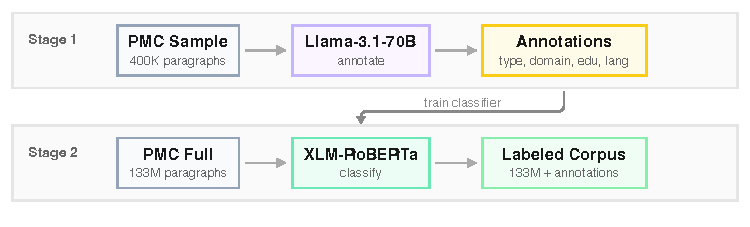
\includegraphics[width=\columnwidth]{sources/part_1/chapter2/imgs/pipeline.pdf}
\caption{\textbf{Two-stage annotation pipeline.} Stage~1: Llama-3.1-70B annotates 0.33\% of PMC paragraphs across four dimensions. Stage~2: a fine-tuned XLM-RoBERTa distills these annotations to label the full corpus, enabling flexible filtering strategies.}
\label{fig:pipeline}
\end{figure}

\subsection{Data Analysis}
\label{sec:data-analysis}

Most PMC paragraphs receive an educational score of 4, with a mean of 3.48 and median of 4.00. This distribution varies by content type: reviews and studies contain the highest proportion of educational content (86.9\% and 78.7\% scoring 4, respectively), while clinical cases show more variance (57.0\% rated 4). Domain-wise, biomedical paragraphs score higher (75.3\% at score 4) than clinical text (44.0\%), and content labeled ``other'' rarely reaches high scores (2.1\%). These patterns support the score threshold ($\geq 3$) used in BE-Educational and BE-All, and explain why combining domain and quality filters yields consistent gains across tasks.

\begin{figure}[t]
\centering
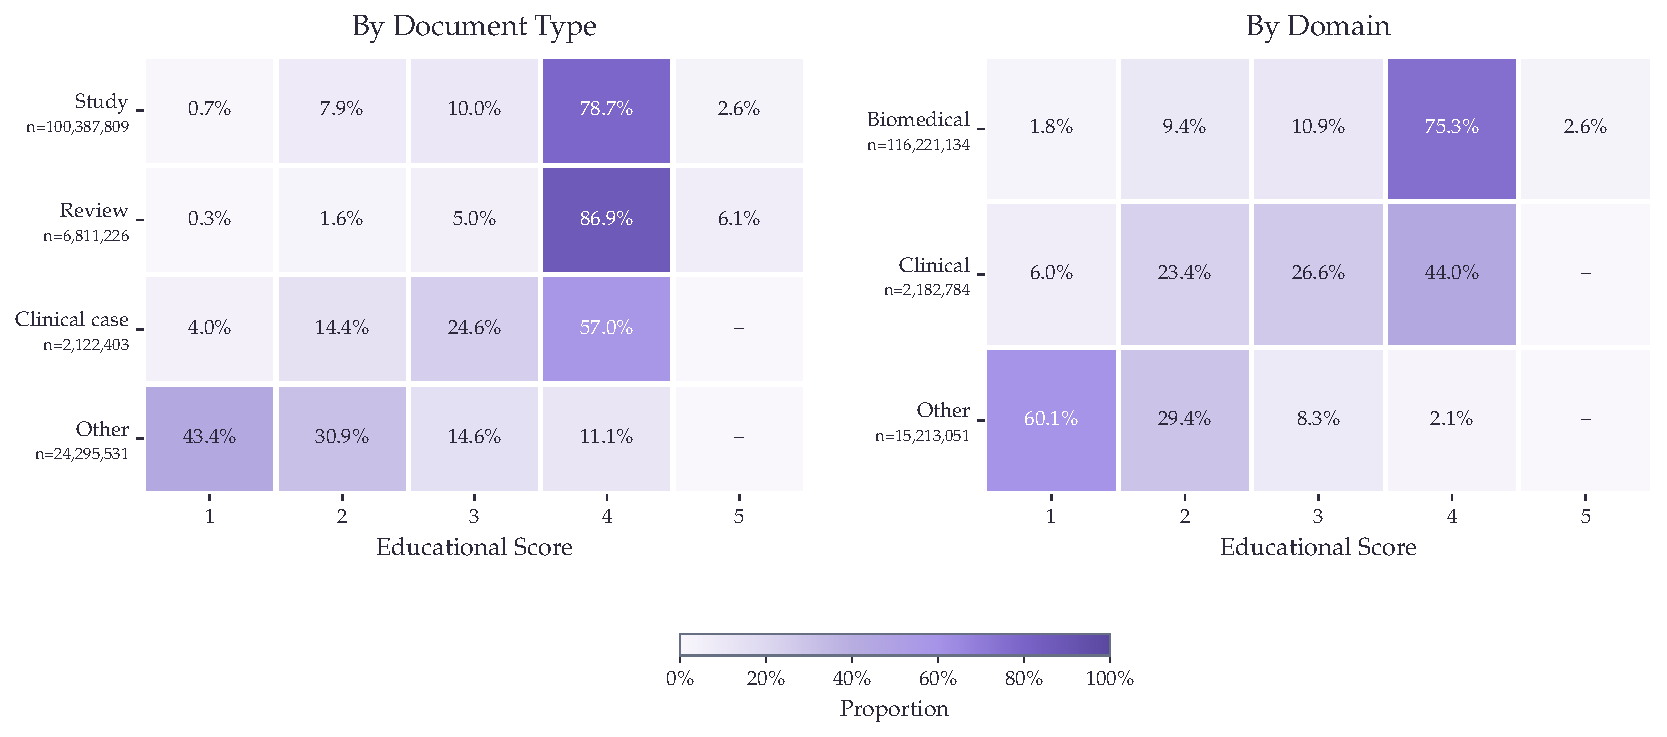
\includegraphics[width=\columnwidth]{plots/chapter2/combined_educational_scores.pdf}
\caption{\textbf{Distribution of educational quality scores by document type and domain.} Reviews and studies show the highest proportion of high scores, while clinical texts display more variance. Content labeled ``other'' rarely reaches high scores.}
\label{fig:edu-scores}
\end{figure}

\subsection{Dataset Construction}
\label{sec:dataset}

Using the distilled model, we annotated the full PMC corpus and constructed several dataset variants through strategic filtering and upsampling, summarized in \Cref{tab:be-variants}. Upsampling refers to duplicating articles in the training corpus, proportionally increasing their sampling probability.

% TODO: add example of a clinical case paragraph extracted from a
% genomics article — showing that clinical content hides in unexpected places

\begin{table}[t]
\centering
\small
\renewcommand{\arraystretch}{1.6}
\begin{tabular}{lp{8.5cm}}
\toprule
\textbf{Variant} & \textbf{Strategy} \\
\midrule
BE-Base & Complete unmodified PMC Open Access Subset (baseline). \\
BE-Educational & Removes paragraphs with educational quality scores below 3. \\
BE-Clinical & Upsamples 10$\times$ articles with predominantly clinical domain content. \\
BE-ClinicalCase & Upsamples 10$\times$ articles containing at least one clinical case paragraph. \\
BE-French & Upsamples 10$\times$ articles containing French text. \\
BE-All & Combines quality filtering (score $\geq 3$), upsampling of clinical content, French text, and clinical cases, plus metadata prefixing. \\
\bottomrule
\end{tabular}
\renewcommand{\arraystretch}{1.0}
\caption{Biomed-Enriched dataset variants. All variants preserve the original article structure and use an 8K context window during pre-training.}
\label{tab:be-variants}
\end{table}

For all variants, we preserved the original structure of the article and employed an 8K context window during pre-training. This ensures that models can process complete scientific articles, capturing dependencies where information presented in earlier paragraphs is essential for understanding later content.


\section{Experimental Setup}
\label{sec:experimental-setup}

Continual pre-training served as a method to evaluate the relevance and utility of our annotations. Our evaluation focuses on isolating the effects of data curation rather than pursuing state-of-the-art scores on benchmarks. A more powerful foundation model would likely yield higher absolute scores, but would probably obscure the precise impact of our dataset.

\subsection{Decoder Setup}

We selected OLMo2-7B-stage1~\citep{olmo2025furious} as our foundation model for continual pre-training, strategically choosing this intermediate checkpoint to more clearly attribute performance changes to our data curation. Although stage~1 has already developed strong language modeling capabilities, it precedes the knowledge-intensive tuning of stage~2, providing an ideal balance of baseline capabilities without the risk of catastrophic forgetting of instruction-following abilities during domain adaptation. Notably, the data mix used in stage~1 includes DCLM~\citep{li2024datacomp}, which is a dataset obtained by filtering web-data using a classifier trained on instruct-data. Hence, OLMo2-7B already has relatively strong question-answering capabilities after stage~1.

Each Biomed-Enriched variant was trained with exactly 33.6 billion tokens, using identical hyperparameters. We follow the annealing strategy of OLMo2 used in the mid-training phase. By maintaining strict parameter parity across experiments, we created a controlled environment focused solely on measuring the effectiveness of our different data curation strategies.

\subsection{Encoder Setup}

We also conducted continual-pretraining experiments on encoder models. Starting from ModernBERT-base~\citep{modernbert} after its context extension phase, we followed exactly the same hyperparameters as BioClinical-ModernBERT phase~1. Our baseline reproduces their standard continual pretraining setup on public PubMed/PMC. Our clinical-upsample recipe additionally applies educational filtering (score $\geq 3$) and upsamples clinical cases 100$\times$ and clinical domain content 10$\times$.

\Cref{tab:hyperparams} summarizes the hyperparameters for both setups.

\begin{table}[t]
\centering
\small
\begin{minipage}[t]{0.48\textwidth}
\centering
\begin{tabular}{ll}
\toprule
\textbf{Parameter} & \textbf{Value} \\
\midrule
Base model & OLMo2-7B-stage1 \\
Peak LR & 6.15e-5 \\
Min LR & 6.15e-6 \\
LR Decay & Linear \\
Batch size & 1024 \\
Weight decay & 0.1 \\
Context & 8,192 tokens \\
Hardware & 128 MI250X \\
Tokens & 33.6B / variant \\
\bottomrule
\end{tabular}
\subcaption{Decoder}
\label{tab:decoder-hyperparams}
\end{minipage}%
\hfill
\begin{minipage}[t]{0.48\textwidth}
\centering
\begin{tabular}{ll}
\toprule
\textbf{Parameter} & \textbf{Value} \\
\midrule
Base model & ModernBERT-base \\
Peak LR & 5e-4 \\
Min LR & 5e-7 \\
LR Decay & one\_minus\_sqrt \\
Batch size & 576 \\
Weight decay & 1e-5 \\
Context & 8,192 tokens \\
Hardware & 4$\times$ H100 \\
Tokens & 70B \\
\bottomrule
\end{tabular}
\subcaption{Encoder}
\label{tab:encoder-hyperparams}
\end{minipage}
\caption{Hyperparameters for continual pre-training.}
\label{tab:hyperparams}
\end{table}

\subsection{Evaluation}

For decoders, our evaluation consists of zero-shot testing on MMLU medical subcategories, MedQA~\citep{jin2021medqa}, MedMCQA~\citep{pal2022medmcqa}, and PubMedQA~\citep{jin2019pubmedqa}. For the French adaptation assessment, we use 5-shot evaluation on FrenchMedMCQA~\citep{labrak-etal-2022}. We compare our models against three baselines: OLMo2-7B-stage1, Llama-3.1-8B, and Meditron-70B.

For the encoder models, we evaluate on 11 tasks spanning clinical and biomedical domains. Clinical tasks include ChemProt, Phenotype, COS, SocialHistory, and DEID. Biomedical tasks include AnatEM, BC5CDR, JNLPBA, NCBI Disease, GAD, and Hallmarks of Cancer. Following the evaluation recipe of BioClinical-ModernBERT, we finetune for 10 epochs on clinical tasks and 20 epochs on biomedical tasks, with early stopping patience of 3 epochs for all. We compare against BioClinical-ModernBERT~\citep{sounack2025bioclinicalmodernbert}, which was trained on 169B tokens from PubMed, PMC, and 20 clinical datasets including MIMIC-III, MIMIC-IV, CheXpert Plus radiology reports, and various clinical notes from multiple institutions, most requiring data use agreements.


\section{Results}
\label{sec:results}

\subsection{Decoder Results}

\Cref{tab:decoder-qa,tab:decoder-mmlu} present decoder results on medical QA and MMLU benchmarks. The combined strategy BE-All achieves the best average performance (61.08\%), with the strongest gains on MedQA (+2.4 pts) and MMLU Clinical Knowledge (+1.5 pts). Different enrichment strategies show complementary strengths: clinical upsampling yields a +4 point improvement on MMLU Professional Medicine, while educational filtering improves Medical Genetics by +2 points and MedMCQA by +1.2 points. BE-All reaches target performance using roughly one-third of the training tokens compared to BE-Base, with stable improvements visible from early checkpoints. BE-French also demonstrates successful adaptation to French medical QA (40.5\% vs 38.3\% baseline, \Cref{fig:french-performance}), showing that language-specific upsampling generalizes beyond English.

\begin{figure}[t]
\centering
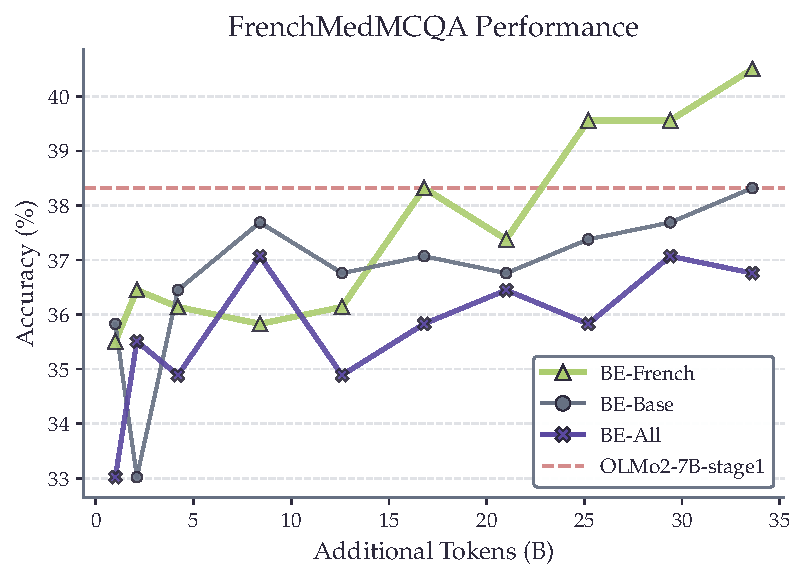
\includegraphics[width=0.55\columnwidth]{plots/chapter2/french_medmcqa_performance.pdf}
\caption{\textbf{FrenchMedMCQA performance.} BE-French outperforms other variants on French medical QA, demonstrating effective language-specific improvement through targeted upsampling.}
\label{fig:french-performance}
\end{figure}

\begin{table}[t]
\centering
\small
\setlength{\tabcolsep}{8pt}
\sisetup{detect-weight=true}
\begin{threeparttable}[b]
\begin{tabular}{l S[table-format=2.2] S[table-format=2.2] S[table-format=2.2] S[table-format=2.2]}
\toprule
\textbf{Model} & {\textbf{MedQA}} & {\textbf{MedMCQA}} & {\textbf{PubMedQA}} & {\textbf{Avg}} \\
\midrule
\rowcolor{ThesisTableSep}
\multicolumn{5}{c}{\rule{0pt}{10pt}\textbf{Reference Models}} \\[1pt]
Llama-3-8B & 59.70 & 57.47 & 74.80 & 63.99 \\
Meditron-70B & 57.10 & 46.80 & 76.60 & 60.17 \\
\midrule
\rowcolor{ThesisTableSep}
\multicolumn{5}{c}{\rule{0pt}{10pt}\textbf{Our Variants}} \\[1pt]
OLMo2-7B-stage1 & 45.33 & 41.14 & 75.60 & 54.02 \\
\quad + BE-Base & 44.85 & 41.91 & 76.40 & 54.39 \\
\quad + BE-Clinical & 41.95 & 39.35 & 76.60 & 52.63 \\
\quad + BE-ClinicalCase & 42.11 & 39.52 & 76.60 & 52.74 \\
\quad + BE-Educational & 45.64 & \bfseries 43.08 & \underline{77.00} & \underline{55.24} \\
\quad + BE-All (33.6B) & \bfseries 47.21 & 42.79 & 76.60 & 55.53 \\
\quad + BE-All (12.6B) & \bfseries 47.21 & \underline{42.94} & 76.40 & \bfseries 55.52 \\
\bottomrule
\end{tabular}
\begin{tablenotes}
  \small
  \item Bold indicates best result per column. Underline: second-best.
\end{tablenotes}
\end{threeparttable}
\caption{\textbf{Decoder results: Medical QA benchmarks.} BE-All achieves the best QA average with both 33.6B and 12.6B tokens.}
\label{tab:decoder-qa}
\end{table}

\begin{table}[t]
\centering
\small
\setlength{\tabcolsep}{6pt}
\sisetup{detect-weight=true}
\begin{threeparttable}[b]
\begin{tabular}{l S[table-format=2.2] S[table-format=2.2] S[table-format=2.2] S[table-format=2.2] S[table-format=2.2] S[table-format=2.2] S[table-format=2.2]}
\toprule
\textbf{Model} & {\textbf{Anat}} & {\textbf{Clin}} & {\textbf{Bio}} & {\textbf{Med}} & {\textbf{Gen}} & {\textbf{Prof}} & {\textbf{Avg}} \\
\midrule
\rowcolor{ThesisTableSep}
\multicolumn{8}{c}{\rule{0pt}{10pt}\textbf{Reference Models}} \\[1pt]
Llama-3-8B & 68.89 & 74.72 & 78.47 & 61.85 & 83.00 & 70.22 & 72.86 \\
Meditron-70B & 53.30 & 66.70 & 76.30 & 63.00 & 69.00 & 71.60 & 66.65 \\
\midrule
\rowcolor{ThesisTableSep}
\multicolumn{8}{c}{\rule{0pt}{10pt}\textbf{Our Variants}} \\[1pt]
OLMo2-7B-stage1 & 54.81 & 63.40 & \underline{69.44} & 53.18 & \underline{69.00} & 59.93 & 61.63 \\
\quad + BE-Base & \underline{57.04} & 64.15 & \bfseries 70.83 & \bfseries 59.54 & \underline{69.00} & 59.93 & 63.42 \\
\quad + BE-Clinical & 53.33 & 63.40 & 65.28 & 58.38 & 66.00 & \bfseries 63.97 & 61.73 \\
\quad + BE-ClinicalCase & 57.04 & 64.91 & 66.67 & \bfseries 59.54 & \underline{69.00} & \underline{62.87} & 63.34 \\
\quad + BE-Educational & 57.04 & \underline{65.28} & 68.06 & 56.65 & \bfseries 71.00 & 58.82 & 62.81 \\
\quad + BE-All (33.6B) & \underline{60.00} & \bfseries 65.66 & 68.06 & \underline{58.96} & \underline{69.00} & 61.40 & \underline{63.85} \\
\quad + BE-All (12.6B) & \bfseries 64.44 & 64.53 & 68.75 & 57.23 & \bfseries 71.00 & \underline{62.87} & \bfseries 64.80 \\
\bottomrule
\end{tabular}
\begin{tablenotes}
  \small
  \item Anat=Anatomy, Clin=Clinical Knowledge, Bio=College Biology, Med=College Medicine, Gen=Medical Genetics, Prof=Professional Medicine.
\end{tablenotes}
\end{threeparttable}
\caption{\textbf{Decoder results: MMLU Medical subcategories.} BE-All (12.6B) achieves the best MMLU average despite using one-third of the tokens.}
\label{tab:decoder-mmlu}
\end{table}

\begin{figure}[t]
\centering
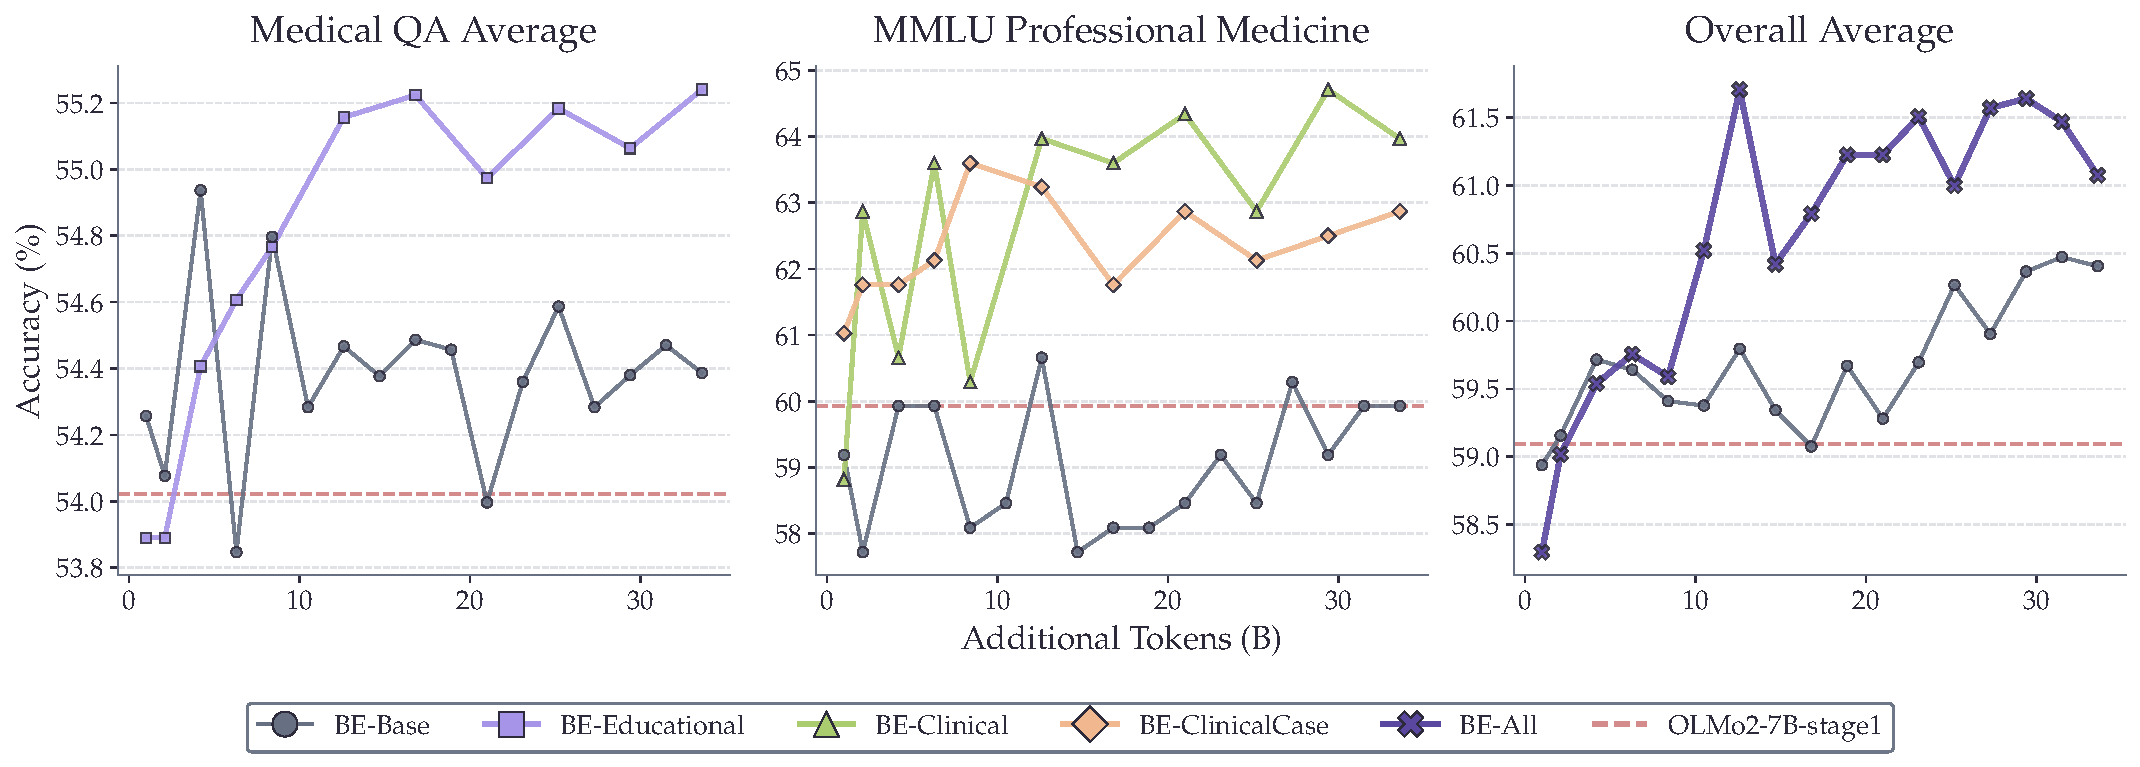
\includegraphics[width=\columnwidth]{plots/chapter2/combined_plot_v2.pdf}
\caption{\textbf{Decoder training progression.} BE-All reaches target performance with approximately one-third of the training tokens required by BE-Base.}
\label{fig:decoder-curves}
\end{figure}

\subsection{Encoder Results}

\Cref{tab:encoder-clinical,tab:encoder-biomed} present encoder results across 11 clinical and biomedical benchmarks. Our BE-Clinical recipe achieves 77.08\% average $F_1$, matching BioClinical-ModernBERT (77.05\%) while using 2.5$\times$ fewer tokens and only public PubMed/PMC data. Adding a decay phase with high-quality educational content brings slight additional gains: the Biomedical decay variant (edu $\geq 4$) achieves 77.32\%.

Different decay targets show task-specific strengths: Study decay yields the best results on AnatEM (79.7\%) and NCBI Disease (81.2\%), Review decay excels on GAD (80.2\%), and Clinical Case decay achieves the highest SocialHistory score (57.0\%). These results suggest that public PMC data has more potential for clinical NLP than commonly exploited, and that targeted curation can close the gap with models trained on restricted datasets.

\begin{table}[t]
\centering
\small
\setlength{\tabcolsep}{6pt}
\sisetup{detect-weight=true}
\begin{threeparttable}[b]
\begin{tabular}{l S[table-format=2.1] S[table-format=2.1] S[table-format=2.1] S[table-format=2.1] S[table-format=2.1] S[table-format=2.1]}
\toprule
\textbf{Model} & {\textbf{ChemPr}} & {\textbf{Pheno}} & {\textbf{COS}} & {\textbf{Social}} & {\textbf{DEID}} & {\textbf{Avg}} \\
\midrule
\rowcolor{ThesisTableSep}
\multicolumn{7}{c}{\rule{0pt}{10pt}\textbf{Baselines}} \\[1pt]
ModernBERT-base & 89.5 & 48.4 & 94.0 & 53.1 & 78.3 & 72.66 \\
BioClinical-MdnBERT\tnote{$\dagger$} & 90.0 & \bfseries 60.7 & 94.8 & 56.0 & \bfseries 81.8 & \bfseries 76.66 \\
\midrule
\rowcolor{ThesisTableSep}
\multicolumn{7}{c}{\rule{0pt}{10pt}\textbf{Our Models (Public Data Only)}} \\[1pt]
Baseline & 89.8 & 59.6 & 94.5 & 55.5 & 78.5 & 75.58 \\
BE-Clinical & 89.9 & 59.9 & 94.8 & 56.8 & 79.7 & 76.22 \\
\midrule
\rowcolor{ThesisTableSep}
\multicolumn{7}{c}{\rule{0pt}{10pt}\textbf{With Decay Phase}} \\[1pt]
\quad + Review & \bfseries 90.3 & 59.7 & 94.6 & 55.4 & 79.6 & 75.92 \\
\quad + Study & \bfseries 90.3 & \bfseries 60.3 & 94.7 & 55.6 & 78.6 & 75.90 \\
\quad + Clinical Case & 89.5 & 59.4 & 94.5 & \bfseries 57.0 & 79.3 & 75.94 \\
\quad + Biomedical & 90.1 & 59.9 & \bfseries 94.9 & 56.4 & 79.6 & \underline{76.18} \\
\bottomrule
\end{tabular}
\begin{tablenotes}
  \small
  \item[$\dagger$] Trained on 169B tokens including 20 clinical datasets (MIMIC-III/IV, CheXpert, etc.). Our models use only public PubMed/PMC.
  \item ChemPr=ChemProt, Pheno=Phenotype, Social=SocialHistory.
\end{tablenotes}
\end{threeparttable}
\caption{\textbf{Encoder results: Clinical tasks.} Our BE-Clinical recipe matches BioClinical-ModernBERT on clinical tasks using only public data.}
\label{tab:encoder-clinical}
\end{table}

\begin{table}[t]
\centering
\small
\setlength{\tabcolsep}{5pt}
\sisetup{detect-weight=true}
\begin{threeparttable}[b]
\begin{tabular}{l S[table-format=2.1] S[table-format=2.1] S[table-format=2.1] S[table-format=2.1] S[table-format=2.1] S[table-format=2.1] S[table-format=2.1]}
\toprule
\textbf{Model} & {\textbf{AnatEM}} & {\textbf{BC5CDR}} & {\textbf{JNLPBA}} & {\textbf{NCBI}} & {\textbf{GAD}} & {\textbf{HoC}} & {\textbf{Avg}} \\
\midrule
\rowcolor{ThesisTableSep}
\multicolumn{8}{c}{\rule{0pt}{10pt}\textbf{Baselines}} \\[1pt]
ModernBERT-base & 77.2 & 87.9 & 74.3 & 77.7 & 76.8 & 66.6 & 76.75 \\
BioClinical-MdnBERT\tnote{$\dagger$} & \bfseries 79.2 & 88.7 & 74.8 & 78.7 & 75.8 & 67.0 & 77.37 \\
\midrule
\rowcolor{ThesisTableSep}
\multicolumn{8}{c}{\rule{0pt}{10pt}\textbf{Our Models (Public Data Only)}} \\[1pt]
Baseline & 78.8 & 88.7 & 74.8 & \bfseries 81.3 & 76.2 & 67.0 & 77.80 \\
BE-Clinical & 78.5 & 88.1 & 74.6 & 79.4 & 77.7 & 68.5 & 77.80 \\
\midrule
\rowcolor{ThesisTableSep}
\multicolumn{8}{c}{\rule{0pt}{10pt}\textbf{With Decay Phase}} \\[1pt]
\quad + Review & 78.5 & 88.5 & 74.7 & 79.6 & \bfseries 80.2 & 68.8 & \underline{78.38} \\
\quad + Study & \bfseries 79.7 & 88.4 & \bfseries 74.8 & 81.2 & 78.7 & 67.7 & \bfseries 78.42 \\
\quad + Clinical Case & 78.7 & 88.3 & 74.7 & 80.0 & 77.9 & 68.1 & 77.95 \\
\quad + Biomedical & 79.0 & \bfseries 88.6 & 74.7 & 79.9 & 78.4 & \bfseries 69.0 & 78.27 \\
\bottomrule
\end{tabular}
\begin{tablenotes}
  \small
  \item[$\dagger$] Same model as \Cref{tab:encoder-clinical}. Trained on 169B tokens with 20 clinical datasets.
\end{tablenotes}
\end{threeparttable}
\caption{\textbf{Encoder results: Biomedical tasks.} Study decay achieves 78.42\%, outperforming BioClinical-ModernBERT (77.37\%) with only public data.}
\label{tab:encoder-biomed}
\end{table}

\begin{figure}[t]
\centering
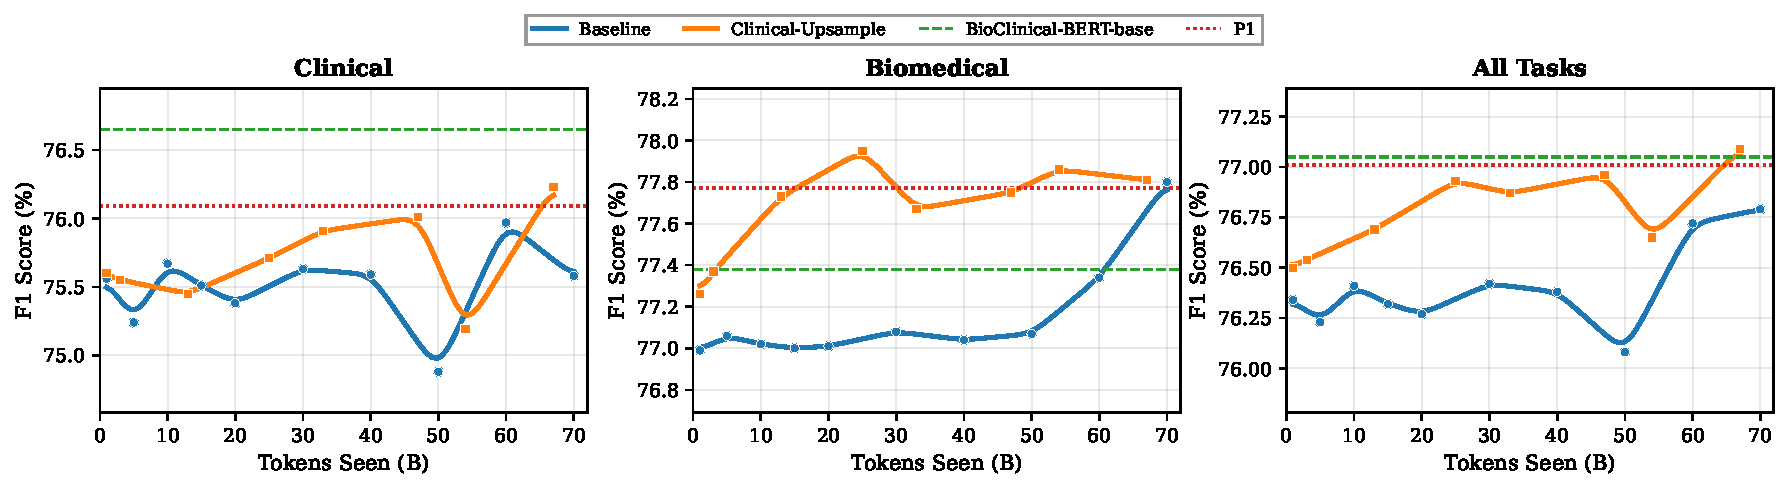
\includegraphics[width=\columnwidth]{sources/part_1/chapter2/imgs/curve_triple.pdf}
\caption{\textbf{Encoder training curves} on clinical, biomedical, and combined benchmarks. Our clinical-upsample recipe (orange) reaches higher performance faster on clinical tasks. At 67B tokens, we match BioClinical-ModernBERT (green dashed) which required 169B tokens and 20 clinical datasets.}
\label{fig:encoder-curves}
\end{figure}


\section{Discussion}
\label{sec:discussion}

The core advantage of paragraph-level annotation lies in its ability to identify valuable content that would be missed by document-level approaches. Clinical case descriptions, for instance, often appear in isolated sections of broader scientific articles. By operating at the paragraph level, we extracted 2 million clinical case paragraphs from PMC Open Access. This content is otherwise difficult to obtain at scale due to privacy restrictions on hospital records.

For decoders, our results reveal clear task-specific benefits from different enrichment strategies. Educational filtering improves knowledge-intensive QA tasks, clinical upsampling enhances clinical reasoning benchmarks, and the combination of both yields the best overall performance with faster convergence. The successful French adaptation through targeted upsampling further demonstrates that this framework generalizes beyond English. However, aggressive clinical upsampling can reduce performance on general biomedical tasks like College Biology, suggesting a trade-off between specialization and breadth.

For encoders, the decay phase experiments reveal that different paragraph types benefit different downstream tasks: Study paragraphs improve NER performance, Clinical Case paragraphs improve social history extraction, and Review paragraphs excel on relation extraction. The distinct task-specific strengths of each decay variant suggest a promising direction: model merging or checkpoint averaging could combine the benefits of specialized training runs without requiring additional compute. Rather than training general-purpose models on massive undifferentiated corpora, these findings support a more modular approach where data composition is tailored to downstream requirements.


\section{The Risks of Neural Quality Filtering}%
\footnote{This section is based on our contribution to \citet{godey_gaperon_2026}.}
\label{sec:biahs}

The results above show that selecting content by type and educational quality can improve pretraining efficiency. A natural next step is to apply neural quality classifiers, as done by FineWeb-Edu~\citep{penedo2024fineweb} and DCLM~\citep{li2024datacomp}, to filter pretraining data more aggressively. However, this raises a question: do these classifiers treat all content equally, or do they have blind spots?

To investigate this, we designed Benchmark-In-A-HayStack (BiaHS), an experiment to test how different text-quality classifiers rank benchmark-like content within a large web corpus. We sampled 35 benchmark instances from three datasets: 15 samples from MMLU (3 samples each from anatomy, computer security, high school geography, moral scenarios, and college physics), 10 from GSM8K~\citep{cobbe2021gsm8k}, and 10 from GPQA~\citep{rein2023gpqa}. Each benchmark sample was formatted as a standalone document containing the question, answer choices, and reference solution. These 35 benchmark documents were inserted as independent entries into a corpus of 99,965 documents sampled from FineWeb, yielding a final evaluation set of 100,000 documents where benchmarks constituted 0.035\% of the total.

We scored all documents using four quality classifiers: DCLM (FastText-based, used to filter OLMo~2 training data), Textbook (FastText-based, used to filter OLMo~1 training data), FineWeb-Edu (transformer-based), and the GAPeron classifier (transformer-based). Each classifier produced a full ranking of all documents based on their predicted quality score.

\begin{figure}[t]
\centering
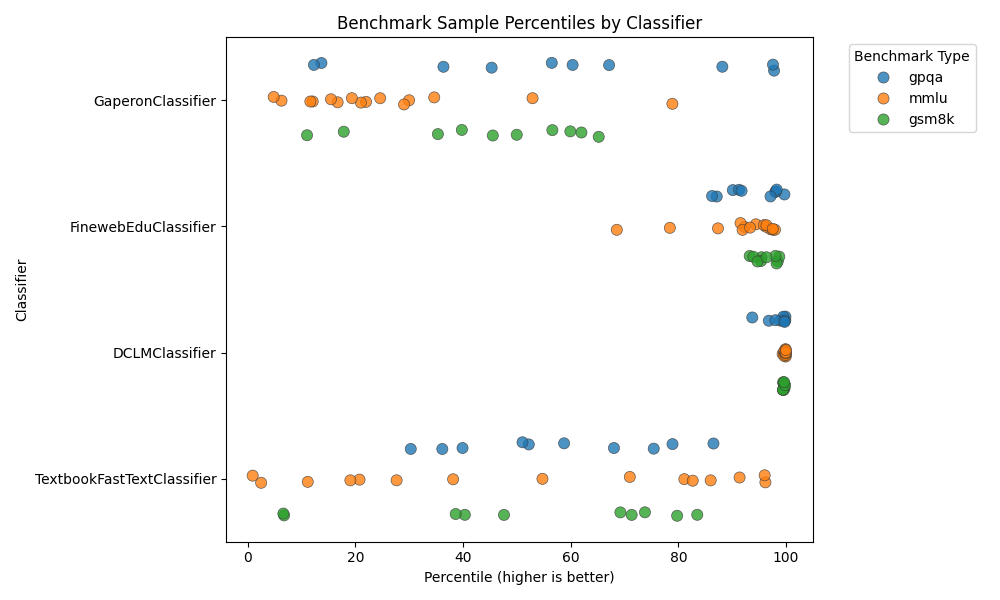
\includegraphics[width=\columnwidth]{sources/part_1/chapter2/imgs/biahs_percentiles.png}
\caption{\textbf{BiaHS: Benchmark-In-A-HayStack results.} Percentile rank of 35 benchmark samples (MMLU, GSM8K, GPQA) within 100K FineWeb documents, as scored by four quality classifiers. DCLM ranks all benchmark samples in the top-5 percentiles.}
\label{fig:biahs}
\end{figure}

The results reveal a striking pattern. The DCLM classifier ranks all MMLU and GSM8K samples in the top-5 percentiles. If only the top 5\% of documents are selected through filtering, the probability of encountering a benchmark sample in a training batch increases by a factor of approximately 20. The FineWeb-Edu classifier also ranks benchmark samples consistently higher, likely because its annotation prompt explicitly asks for documents with high educational value, which naturally favors exam-style items and step-by-step solutions.

The DCLM classifier pushes benchmark samples even higher and more consistently. Its FastText model is trained to separate synthetically generated instructions from high-scoring Reddit posts, from general web text. This training objective naturally favors solved Q\&A structures with a short question, a direct answer, and brief reasoning, which aligns with the format of common benchmark datasets.

In contrast, the GAPeron classifier does not significantly push benchmark samples. It was trained on annotations focused on general content quality across multiple dimensions: accuracy, clarity, coherence, grammar, depth of information, and overall usefulness. This broader framing does not specifically reward the structured question-answer format typical of benchmark samples.

\paragraph{Implications.} This experiment suggests that the way quality classifiers are trained can strongly influence contamination risks. As neural quality filtering becomes a standard step in data curation, these design choices deserve closer examination. For the Biomed-Enriched work presented earlier in this chapter, we rely on content-type classification and educational quality scoring rather than general quality filtering, which avoids this particular risk.


\section{Limitations}

Our decoder experiments used 7B parameter models. Larger models may respond differently to data curation choices. The two-stage annotation pipeline relies on XLM-RoBERTa-base, which may have limited capacity for nuanced paragraph classification. Our clinical case paragraphs come from published case reports, which may differ stylistically from actual hospital records. The educational quality scores are neural heuristics rather than gold-standard pedagogical assessments.

For the BiaHS experiment, the evaluation was conducted on a relatively small number of benchmark samples (35) inserted into a single web corpus (FineWeb). While the results are directionally clear, a larger-scale study across multiple corpora would strengthen the conclusions.


\section*{Conclusion}

Two findings emerge from this chapter. First, paragraph-level annotation reveals that scientific articles are far more heterogeneous than their metadata suggests: 91.6\% mix content types, and educational quality varies by 2.6 points within a single article. Selecting the right paragraphs allows matching full-corpus performance with a third of the tokens, and extracting 2 million clinical case paragraphs provides public clinical text without data use agreements.

Second, not all filtering is created equal. Neural quality classifiers trained on instructional or educational content can amplify benchmark contamination by a factor of 20, effectively turning a data curation step into a memorization accelerator. Content-type classification, by contrast, selects for relevance rather than format, and does not carry this risk.

\vspace{2em}

We now have both a general biomedical corpus (\textit{biomed-fr}, \Cref{chap:collecting}) and a method for selecting the most relevant paragraphs within it. The next chapter addresses how to combine these resources into a curated training mix, and how quality signals can be used at scale to build a better corpus for pretraining ModernCamemBERT-bio.


\chapter{Which Quality Signals Matter?}
\label{chap:mcbio}
% This chapter is based on the corpus contribution of:
%   Rian Touchent, Éric de la Clergerie.
%   ModernCamemBERT-bio: un encodeur biomédical et clinique français à contexte long.
%   TALN 2026.
%
% Source: publications/TALN2026_MB-BIO/
% This chapter covers only the corpus (biomed-fr-v2). The pretraining and evaluation
% are presented in \Cref{chap:objectives}.

\section{Introduction}

Here is one passage as it came out of an ISTEX PDF:

\begin{quote}\small\ttfamily
\dots{} vise \textasciitilde{} remonter l\&apos;organe prolab6 (correction de la pt6se) et h le soutenir dans sa position id6ale plus qu\&apos;/\textasciitilde{} le fixer (fixation). Ce sout\textasciitilde{}nement est assur6 par le renforcement du p6rin6e grace aux tissus naturels que l\&apos;on r6pare (rapphie) ou que l\&apos;on consolide avec du mat6riel local (plastie, ligamentopexie)\dots{}
\end{quote}

\noindent And here is what it should read:

\begin{quote}\small
\dots{} la chirurgie vise à remonter l'organe prolapsé (correction de la ptose) et à le soutenir dans sa position idéale plus qu'à le fixer (fixation). Ce soutien est assuré par le renforcement du périnée grâce aux tissus naturels que l'on répare (raphie) ou que l'on consolide avec du matériel local (plastie, ligamentopexie)\dots{}
\end{quote}

\noindent OCR had read every \emph{é} as a \emph{6}, apostrophes came as \texttt{l\&apos;}, and tildes had drifted into the middle of words. Multiply this by the hundreds of thousands of similar PDFs in HAL and ISTEX, and assembling a 10-billion-token biomedical training mixture stops being a collection problem and becomes a repair problem.

\Cref{chap:collecting} introduced \textit{biomed-fr}, a 413-million-word public French biomedical corpus. \Cref{chap:quality} showed that paragraph-level annotation by a large language model can identify content types and educational quality more precisely than document-level filters, and that neural quality classifiers carry contamination risks. This chapter applies these lessons at scale. We assemble \textit{biomed-fr-v2}, a 10-billion-token mixture from six French sources, and ask which quality signals actually improve downstream performance once the dust settles. The corpus is the training data for ModernCamemBERT-bio, presented in \Cref{chap:objectives}.

The contributions of this chapter are: (1) a multi-source French biomedical corpus 25 times larger than \textit{biomed-fr}, including a curation pipeline that handles the OCR artifacts, boilerplate, and structural noise of HAL and ISTEX; (2) an LLM-based annotation of 2.16 million paragraphs along four quality signals and nine content types; (3) ablation studies that quantify the effect of each signal and each type on downstream performance, with one notable surprise: writing-quality and terminological-precision filters \emph{degrade} performance.


\section{Sources}
\label{sec:corpus-sources}

We assemble \textit{biomed-fr-v2} from six complementary French-language sources. HAL, ISTEX, and FineWiki-bio cover scientific biomedical literature. EMEA contributes drug package inserts. E3C contributes clinical case reports. Synthetic textbooks generated from medical ontologies complete the mixture with the vocabulary of French administrative nomenclatures. The final composition is summarized in \Cref{tab:mcbio-corpus}.

\begin{itemize}
\item \textbf{HAL.} Medical theses, research articles, and reports deposited on the HAL open archive, filtered to the biomedicine section.
\item \textbf{ISTEX.} French scientific articles from the ISTEX corpus, filtered to biology and medicine.
\item \textbf{FineWiki-bio.} Biomedical subset of FineWiki, the Wikipedia counterpart to FineWeb~\citep{penedo2024fineweb}, restricted to French and filtered for the biomedical domain.
\item \textbf{EMEA}~\citep{neveol14quaero}. Drug package inserts published in French by the European Medicines Agency.
\item \textbf{E3C}~\citep{magnini_e3c_2021}. Multilingual clinical corpus (layer 3, French partition), composed of clinical cases extracted from medical journals and theses.
\item \textbf{Synthetic ontology textbooks.} Educational text generated from three French medical ontologies published by the Agence du Numérique en Santé in RDF/OWL format: CIM-10 (diagnoses, 19{,}161 codes), CCAM (procedures, 38{,}191 codes), and ATC (medications, 6{,}950 codes). Random walks through the ontology graph (1.3 million walks total) traverse hierarchical relations and, for CIM-10, causal and exclusion relations. A large language model (Qwen3-235B-A22B-Instruct) reformulates each walk into a paragraph of medical prose while preserving the original codes and relations. The full pipeline is described in \Cref{chap:ontobook}.
\end{itemize}

HAL and ISTEX are distributed in heterogeneous formats: some documents come with structured XML, others only as PDFs, sometimes scans of printed material. For documents without clean XML, we apply the extraction and cleaning pipeline described in \Cref{sec:corpus-pipeline}. FineWiki-bio, EMEA, E3C, and the synthetic textbooks are already of high quality and are integrated directly into the final mixture, bypassing this pipeline.


\section{Curation Pipeline}
\label{sec:corpus-pipeline}

A portion of HAL and ISTEX documents come with clean XML and proceed directly to annotation. The other portion is available only as PDFs, sometimes scans of printed material (particularly for articles published before the 1990s). Once converted to text, these PDFs contain OCR artifacts (incorrect ligatures, character substitutions, fragmented words), bibliographic references, repeated headers, and irrelevant content. We therefore apply an LLM-based extraction and cleaning pipeline, described below. The other sources (FineWiki-bio, EMEA, E3C, synthetic textbooks) are already clean and bypass this pipeline entirely.

\paragraph{Extraction and cleaning.} Each document is split into segments of approximately 5{,}000 tokens at paragraph boundaries. A large language model (Qwen3-Next-80B-A3B-Instruct) receives each segment and produces structured JSON output containing semantically complete passages, with references, metadata, headers, and captions removed, and OCR errors corrected (ligatures, encoding). Extracted passages must contain between 30 and 600 words and at least 60\% alphabetic characters. We then apply Jaccard-similarity deduplication (threshold 0.80, sliding window of 5 passages), followed by the FineWeb-2 filter chain for French: encoding correction, repetition filters, and Gopher and FineWeb quality filters.

\paragraph{Fidelity verification.} To ensure the LLM does not introduce content absent from the source, we measure character-level overlap between each extracted passage and its source document on 300 ISTEX passages (after typographic normalization). 94.4\% of passages have $\geq 90$\% overlap and 84.1\% have $\geq 99$\% overlap; the median rate of words absent from the source is zero (mean: 3.4\%). Manual inspection of edge cases shows that divergences come from OCR corrections (such as the surgical passage shown at the start of this chapter) or from converting tables into prose. The opposite case is also common: a clean 1{,}143-character passage on cancer-related depression is extracted with 100\% character overlap and no additional words introduced. These two cases bracket the typical behavior of the pipeline: it cleans aggressively when the source is corrupted by OCR, and copies verbatim when the source is already clean.

\paragraph{LLM quality annotation.} The same LLM annotates each passage along four quality signals scored from 1 to 10: educational value (\texttt{edu}, mean 6.5), content richness (\texttt{cont}, 6.8), writing quality (\texttt{writ}, 7.6), and terminological precision (\texttt{term}, 7.6). The codes in parentheses are the abbreviations used in ablation tables. A content type is also assigned among nine categories: \texttt{research\_findings} (526k passages), \texttt{medical\_knowledge} (388k), \texttt{clinical\_guidance} (218k), \texttt{research\_methodology}, \texttt{drug\_information}, \texttt{background\_review}, \texttt{policy\_administrative}, \texttt{patient\_case} (36k), and \texttt{other}. In total, 2.16 million passages are annotated.


\section{Content-Type Ablation}

We measure the effect of each content type by ablation: we remove one type and compare against the full corpus on three evaluation tasks (DiaMed, FrACCO-30, and EMEA, 9 seeds). \Cref{tab:mcbio-content-type} shows that removing \texttt{drug\_information} \emph{improves} performance by $+0.67$pp, while removing \texttt{medical\_knowledge} degrades it by $-0.13$pp. A random control (removing the same amount of text at random) gives $+0.04$pp, confirming that the effect is specific to the content type.

\begin{table}[t]
\centering
\small
\setlength{\tabcolsep}{8pt}
\begin{tabular}{lcc}
\toprule
\textbf{Type removed} & \textbf{Avg $F_1$} & $\boldsymbol{\Delta}$ \\
\midrule
\rowcolor{ThesisTableSep}
\multicolumn{3}{c}{\rule{0pt}{10pt}\textbf{Removal helps}} \\[1pt]
\texttt{drug\_information} & 64.35 & $+$0.67pp \\
\texttt{research\_findings} & 64.24 & $+$0.56pp \\
\texttt{policy\_administrative} & 64.07 & $+$0.39pp \\
\midrule
\rowcolor{ThesisTableSep}
\multicolumn{3}{c}{\rule{0pt}{10pt}\textbf{Controls}} \\[1pt]
Random (same volume) & 63.72 & $+$0.04pp \\
Full corpus (reference) & 63.68 & ref. \\
\midrule
\rowcolor{ThesisTableSep}
\multicolumn{3}{c}{\rule{0pt}{10pt}\textbf{Removal hurts}} \\[1pt]
\texttt{medical\_knowledge} & 63.55 & $-$0.13pp \\
\texttt{research\_methodology} & 63.51 & $-$0.17pp \\
\bottomrule
\end{tabular}
\caption{\textbf{Content-type ablation.} We remove one type and measure $\Delta$ relative to the full corpus.}
\label{tab:mcbio-content-type}
\end{table}

We exclude \texttt{drug\_information} from the final corpus (redundant with the EMEA source already included separately) and \texttt{other}. Paragraphs shorter than 50 tokens are also excluded.


\section{Quality Filtering and Upsampling}
\label{sec:upsampling}

We then test the effect of thresholding on the quality signals (\Cref{tab:mcbio-quality-signals}). Joint filtering with \texttt{edu}$\geq 7$ and \texttt{cont}$\geq 7$ produces a $+0.48$pp gain; a stricter threshold (\texttt{edu}$\geq 8$ and \texttt{cont}$\geq 8$) reaches $+0.55$pp. By contrast, the writing-quality and terminological-precision signals \emph{degrade} performance when used as filters ($-0.26$ and $-0.33$pp). This degradation likely comes from the fact that these filters eliminate informal but informative clinical documents, such as case notes and lightly edited reports.

\begin{table}[t]
\centering
\small
\setlength{\tabcolsep}{8pt}
\begin{tabular}{lcc}
\toprule
\textbf{Filter} & \textbf{Avg $F_1$} & $\boldsymbol{\Delta}$ \\
\midrule
\rowcolor{ThesisTableSep}
\multicolumn{3}{c}{\rule{0pt}{10pt}\textbf{Helpful filters}} \\[1pt]
\texttt{edu}$\geq 8$ AND \texttt{cont}$\geq 8$ & \bfseries 59.37 & $+$0.55pp \\
\textbf{\texttt{edu}$\geq 7$ AND \texttt{cont}$\geq 7$} & \underline{59.30} & \textbf{$+$0.48pp} \\
\texttt{edu}$\geq 6$ AND \texttt{cont}$\geq 6$ & 58.95 & $+$0.13pp \\
\midrule
No filter (reference) & 58.82 & ref. \\
\midrule
\rowcolor{ThesisTableSep}
\multicolumn{3}{c}{\rule{0pt}{10pt}\textbf{Harmful filters}} \\[1pt]
\texttt{term}$\geq 7$ & 58.57 & $-$0.26pp \\
\texttt{writ}$\geq 7$ & 58.49 & $-$0.33pp \\
\bottomrule
\end{tabular}
\caption{\textbf{Quality-signal ablation.} Educational value and content richness improve performance; writing quality and terminological precision degrade it.}
\label{tab:mcbio-quality-signals}
\end{table}

Rather than applying a strict filter, we adopt a quality-weighted upsampling inspired by FineWeb~\citep{penedo2024fineweb}. Each article receives a quality ratio, defined as the proportion of its paragraphs satisfying \texttt{edu}$\geq 7$ AND \texttt{cont}$\geq 7$. Articles are then upsampled in proportion to this ratio (\Cref{tab:mcbio-upsampling}). Articles with 0\% high-quality paragraphs are excluded from the final corpus.

\begin{table}[t]
\centering
\small
\setlength{\tabcolsep}{12pt}
\begin{tabular}{lr}
\toprule
\textbf{Ratio of \texttt{edu}$\geq 7$ AND \texttt{cont}$\geq 7$ paragraphs} & \textbf{Coefficient} \\
\midrule
0\% & excluded \\
1--25\% & 4.3$\times$ \\
26--50\% & 8.5$\times$ \\
51--75\% & 12.8$\times$ \\
76--99\% & 21.3$\times$ \\
100\% & 34.1$\times$ \\
\bottomrule
\end{tabular}
\caption{\textbf{Upsampling coefficients} per article-quality bucket.}
\label{tab:mcbio-upsampling}
\end{table}


\section{Final Composition}

The final training mixture, after cleaning and quality-weighted upsampling, contains 10 billion tokens (\Cref{tab:mcbio-corpus}). These 10 billion include the repetitions induced by upsampling (coefficients ranging from 4.3$\times$ to 34.1$\times$ depending on quality, see \Cref{sec:upsampling}); the underlying unique content is more limited. HAL and ISTEX articles (passed through the pipeline of \Cref{sec:corpus-pipeline}) and FineWiki-bio (integrated as-is) are grouped under ``curated biomedical articles.'' The three other sources (EMEA, E3C, synthetic textbooks) are also integrated as-is.

\begin{table}[t]
\centering
\small
\setlength{\tabcolsep}{10pt}
\begin{tabular}{lrrl}
\toprule
\textbf{Source} & \textbf{Tokens} & \textbf{\%} & \textbf{Content} \\
\midrule
Curated biomedical articles & 7B & 70\% & HAL + ISTEX + FineWiki-bio \\
Synthetic ontology textbooks & 2B & 20\% & CIM-10, CCAM, ATC \\
EMEA (drug inserts) & 600M & 6\% & Pharmacology \\
E3C (clinical sentences) & 400M & 4\% & Patient cases \\
\midrule
\textbf{Total} & \textbf{10B} & \textbf{100\%} & \\
\bottomrule
\end{tabular}
\caption{\textbf{Composition of the \textit{biomed-fr-v2} training mixture} after quality-weighted upsampling.}
\label{tab:mcbio-corpus}
\end{table}


\section*{Conclusion}

Two findings emerge from the ablations. First, not all content types contribute equally: removing drug information actually improves downstream performance, while removing medical knowledge degrades it. Second, not all quality signals work as filters: educational value and content richness help, but writing-quality and terminological-precision filters \emph{hurt} performance, likely because they remove the informal but informative clinical documents that ultimately matter most. The lesson, perhaps, is that curation should be guided by what is being said, not by how well it is written.

\vspace{2em}

The corpus is now ready. The next two chapters use it to train French biomedical encoders. \Cref{chap:encoders} starts with the simplest recipe (continual pretraining with MLM on \textit{biomed-fr}) and shows that even a modest public corpus produces a competitive model. \Cref{chap:objectives} returns to \textit{biomed-fr-v2} with a more ambitious recipe: a temporary detour through causal language modeling that, somewhat unexpectedly, leaves a permanent imprint on the encoder.




\illustratedpart[Pretraining Language Models]{Pretraining Language Models}%
  {static/part-openers/ramelli-bookwheel.jpg}%
  {\partplatecaption
    {A rotating bookcase allows one person to read multiple books with ease.}
    {Agostino Ramelli, bookwheel from
     \emph{Le diverse et artificiose machine}, 1588.}}
\label{part:pretraining}
\chapter{Encoder Models for French Biomedicine}
\label{chap:encoders}
\partepigraph{``I'd taught him new words that he'd held there in his mind like
jewels, and repeated over and over until he knew them better than I did.''}{%
Jeff VanderMeer, \textit{Borne}}
% This chapter is based on the pretraining contribution of:
%   Rian Touchent, Laurent Romary, Éric de la Clergerie.
%   CamemBERT-bio: Leveraging Continual Pre-training for
%   Cost-Effective Models on French Biomedical Data.
%   LREC-COLING, 2024.
%
% The corpus construction is presented in \Cref{chap:collecting}.

\section{Introduction}

In \Cref{chap:collecting}, we found that 55\% of biomedical subwords are absent from CamemBERT's vocabulary. PubMedBERT~\citep{gu_domain-specific_2022} turned this kind of observation into a principle: for domains with enough unlabeled text, training a language model from scratch with a specialized vocabulary outperforms continual pretraining. The gain over BioBERT~\citep{lee_biobert_2019} was modest, but the conclusion was adopted widely.

For French, \citet{labrak2023drbert} went further. They reported that continual pretraining from CamemBERT led to $F_1$ losses of up to 20 points, and released DrBERT, trained from scratch on 128 V100 GPUs for 20 hours. The claim was strong, the compute was expensive, and the implication was clear: continual pretraining does not work for French biomedical models. Yet the size of the reported loss is difficult to reconcile with what we know about continual pretraining. A model that has already seen 138\,GB of French text should not lose 20 points from seeing additional biomedical text. Something in the evaluation deserves closer examination.

In this chapter, we show that continual pretraining on \textit{biomed-fr} (\Cref{chap:collecting}) yields an average improvement of +2.54 $F_1$ across five biomedical NER benchmarks, using 2 V100 GPUs for 39 hours. We also identify the methodological differences that led to the contradictory conclusion.


\section{Pre-training}

For the adaptation of CamemBERT to the biomedical domain, we conducted a second phase of pre-training on both versions of the \textit{biomed-fr} corpus, starting from the weights and configuration of the camembert-base model. We applied the Masked Language Modeling (MLM) task with whole-word masking, following the method of \citet{martin-etal-2020-camembert}. We used the Adam optimizer~\citep{kingma_adam_2017} with $\beta_1 = 0.9$ and $\beta_2 = 0.98$, and a learning rate of $5 \times 10^{-5}$. We performed 50,000 steps over 39 hours using two Tesla V100 GPUs. A batch size of 8 per GPU and gradient accumulation over 16 steps were used to achieve an effective batch size of 256.


\section{Fine-tuning and Evaluation}

Regarding model evaluation, we collected three named entity recognition evaluation datasets. These datasets cover various styles, allowing us to assess the model's versatility across different subdomains of biomedicine.

\paragraph{QUAERO.} The QUAERO corpus~\citep{neveol14quaero} consists of two evaluation sets: EMEA, containing drug leaflets, and MEDLINE, containing scientific article titles. The entities are manually annotated following 10 semantic groups from the UMLS~\citep{lindberg_unified_1993}. As some of these entities are nested, we kept only the entities with the coarsest granularity.

\paragraph{E3C.} For evaluation, unlike the \textit{biomed-fr} corpus, we use layers 1 and 2. These layers contain documents of different types, including clinical cases extracted from scientific articles. Layer 2 is semi-annotated, and it is used as the training set for fine-tuning, with 10\% dedicated to the validation set. We evaluate on layer 1, which is fully manually annotated. There is only one class, and the objective is to find clinical entities in the text, regardless of their type.

\paragraph{CAS.} The CAS corpus~\citep{grouin_clinical_2019} also consists of clinical cases from scientific articles. We focus on task 3 of DEFT 2020~\citep{cardon_presentation_2020}, which is an information extraction task based on CAS. It includes two subtasks, and thus two sets of annotations. In the first subtask, two classes need to be identified: \textit{pathology} and \textit{signs or symptoms}. The second subtask concerns associated information, including \textit{anatomy}, \textit{dose}, \textit{examination}, \textit{mode}, \textit{timing}, \textit{substance}, \textit{treatment}, and \textit{value}. These two tasks will be referred to as CAS1 and CAS2, respectively.

\paragraph{Fine-tuning.} For fine-tuning, we used Optuna~\citep{akiba_optuna_2019} for hyperparameter selection. We set the learning rate to $5 \times 10^{-5}$, the warmup ratio to 0.224, and the batch size to 16. We performed 2000 steps. Predictions were made using a simple linear layer on top of the model. None of the CamemBERT layers were frozen.

\paragraph{Evaluation.} Scores are measured using the seqeval tool~\citep{seqeval} in strict mode with micro-average and the IOB2 scheme. For each evaluation, the best fine-tuned model on the validation set is selected to measure the final score on the test set. We average the results over 10 evaluations with different seeds.


\section{Results and Discussion}

\begin{table}[t]
\centering
\small
\setlength{\tabcolsep}{5pt}
\sisetup{detect-weight=true}
\begin{threeparttable}[b]
\begin{tabular}{l S[table-format=2.2] S[table-format=2.2] S[table-format=2.2]}
\toprule
& & \multicolumn{2}{c}{\textbf{CamemBERT-bio}} \\
\cmidrule(lr){3-4}
\textbf{Dataset} & {\textbf{CamemBERT}} & {\textbf{biomed-fr-small}} & {\textbf{biomed-fr}} \\
\midrule
\rowcolor{ThesisTableSep}
\multicolumn{4}{c}{\rule{0pt}{10pt}\textbf{Clinical}} \\[1pt]
CAS1 & 70.50 & \underline{72.94} & \bfseries 73.03 \\
CAS2 & 79.02 & \underline{80.00} & \bfseries 81.66 \\
E3C  & 67.63 & \underline{67.96} & \bfseries 69.85 \\
\midrule
\rowcolor{ThesisTableSep}
\multicolumn{4}{c}{\rule{0pt}{10pt}\textbf{Leaflets}} \\[1pt]
EMEA & 74.14 & \underline{75.93} & \bfseries 76.71 \\
\midrule
\rowcolor{ThesisTableSep}
\multicolumn{4}{c}{\rule{0pt}{10pt}\textbf{Scientific}} \\[1pt]
MEDLINE & \underline{65.73} & 65.48 & \bfseries 68.47 \\
\midrule
\textbf{Average} & 71.40 & \underline{72.46} & \bfseries 73.94 \\
\bottomrule
\end{tabular}
\begin{tablenotes}
  \small
  \item $F_1$ scores (micro-average, seqeval strict, IOB2). Mean over 10 seeds. biomed-fr-s = biomed-fr-small (10\% subset).
\end{tablenotes}
\end{threeparttable}
\caption{\textbf{CamemBERT vs CamemBERT-bio} on five biomedical NER benchmarks. Continual pretraining on \textit{biomed-fr} yields +2.54 $F_1$ on average.}
\label{tab:bioVSbase}
\end{table}

\paragraph{CamemBERT vs CamemBERT-bio.} We observe a significant performance gain on all evaluation datasets with our new model (\Cref{tab:bioVSbase}). On average, we achieve a 2.54-point improvement in F-score. This gain is observed across all styles, demonstrating the model's versatility for both clinical and scientific domains.

\paragraph{biomed-fr-small vs biomed-fr.} We observe a decrease in performance with the biomed-fr-small dataset, but there is still a significant gain on certain datasets compared to CamemBERT. This confirms that the size of the corpus positively influences the performance, even in a specialized domain like biomedicine.

\paragraph{Comparison with the state of the art.} We compared the performance of CamemBERT-bio with various previously mentioned approaches (\Cref{tab:compare}). CamemBERT-bio achieves the best results for almost all evaluation datasets. \citet{dura_learning_2022} did not observe improvement on EMEA and MEDLINE compared to CamemBERT because their pre-training corpus consists of documents from APHP, making it a less diverse corpus. However, they gain several points on their evaluation dataset, which is also based on APHP documents. \citet{mulligen_erasmus_2016} presents the highest score on MEDLINE and the best recall on EMEA. Their approach is based on a knowledge-based model, allowing them to achieve the best recall on both QUAERO evaluation datasets. Furthermore, their approach is the only one in this table capable of handling nested entities, giving them an advantage.

It is important to note that these different CamemBERT-based approaches have various experimental setups. The presence of CRF layers instead of a simple linear layer after CamemBERT, freezing CamemBERT layers, and variations in hyperparameters are examples of differences observed in addition to the pre-training corpus, which makes the comparison more challenging.

\begin{table}[t]
\centering
\small
\setlength{\tabcolsep}{4pt}
\sisetup{detect-weight=true}
\begin{threeparttable}[b]
\begin{tabular}{l S[table-format=2.2] S[table-format=2.2] S[table-format=2.2] S[table-format=2.2]}
\toprule
\textbf{Authors} & {\textbf{CAS1}} & {\textbf{CAS2}} & {\textbf{EMEA}} & {\textbf{MEDLINE}} \\
\midrule
\rowcolor{ThesisTableSep}
\multicolumn{5}{c}{\rule{0pt}{10pt}\textbf{seqeval}} \\[1pt]
\citet{dura_learning_2022} & {--} & {--} & \underline{72.90} & 59.70 \\
Ours & \bfseries 73.03 & \bfseries 81.66 & \bfseries 76.71 & \bfseries 68.47 \\
\midrule
\rowcolor{ThesisTableSep}
\multicolumn{5}{c}{\rule{0pt}{10pt}\textbf{BRATeval}} \\[1pt]
\citet{le_clercq_de_lannoy_strategies_2022} & {--} & {--} & 67.40 & 55.30 \\
\citet{mulligen_erasmus_2016} & {--} & {--} & \underline{74.90} & \bfseries 69.80 \\
\citet{copara_contextualized_2020} & \underline{61.53} & \underline{73.70} & {--} & {--} \\
Ours & \bfseries 84.97 & \bfseries 83.25 & \bfseries 77.80 & \underline{56.16} \\
\bottomrule
\end{tabular}
\begin{tablenotes}
  \small
  \item $F_1$ scores. BRATeval is the evaluation tool from the CLEF eHealth 2016 campaign~\citep{neveol_clinical_2016}.
\end{tablenotes}
\end{threeparttable}
\caption{\textbf{Comparison with existing approaches} on four NER tasks, using two evaluation tools.}
\label{tab:compare}
\end{table}


\section{Evaluating Models: Methodology Matters}

In a recent work, \citet{labrak2023drbert} introduced a new French biomedical language model named DrBERT. The authors contend that performing continual-pretraining on biomedical data from CamemBERT leads to reduced performance. They used a different methodology for the evaluation of named entity recognition, prompting us to examine the implications of each approach on the interpretation of the results.

Our evaluation approach is centered around micro $F_1$, which is measured using seqeval in strict mode with the IOB2 scheme. Their approach is based on weighted $F_1$ with independent token classification. Every token has a label and the model is evaluated for each of them, whereas with seqeval, the model is evaluated for each entity. Notably, the ``O'' token, representing non-entity, is the most frequent token and thus holds significant weight in the evaluation process. As all tokens are labeled, the number of predictions depends on the tokenizer, thereby influencing the final score.

In order to explore the impact of token labeling variations on the evaluation, we conducted an additional experiment on EMEA and MEDLINE where we reproduced the DrBERT methodology that we named \textit{token-with-O}, and another one where we excluded the ``O'' token and only labeled the first token of each entity, referred to as \textit{entity-without-O}.

\begin{table}[t]
\centering
\small
\setlength{\tabcolsep}{3pt}
\sisetup{detect-weight=true}
\begin{threeparttable}[b]
\begin{tabular}{ll S[table-format=2.2] S[table-format=2.2] S[table-format=2.2] S[table-format=2.2]}
\toprule
& & \multicolumn{2}{c}{\textbf{EMEA}} & \multicolumn{2}{c}{\textbf{MEDLINE}} \\
\cmidrule(lr){3-4} \cmidrule(lr){5-6}
\textbf{Method} & \textbf{Model} & {\textbf{w-$F_1$}} & {\textbf{m-$F_1$}} & {\textbf{w-$F_1$}} & {\textbf{m-$F_1$}} \\
\midrule
\rowcolor{ThesisTableSep}
\multicolumn{6}{c}{\rule{0pt}{10pt}\textbf{token-with-O}} \\[1pt]
& DrBERT-7GB & 87.45 & 34.95 & 75.52 & \bfseries 15.07 \\
& CamemBERT-bio & \bfseries 90.37 & \underline{36.27} & \bfseries 77.89 & \underline{14.82} \\
& CamemBERT & \underline{88.33} & \bfseries 47.45 & \underline{76.20} & 11.92 \\
\midrule
\rowcolor{ThesisTableSep}
\multicolumn{6}{c}{\rule{0pt}{10pt}\textbf{entity-without-O}} \\[1pt]
& DrBERT-7GB & 66.72 & \bfseries 24.72 & 60.70 & \bfseries 10.80 \\
& CamemBERT-bio & \bfseries 73.53 & \underline{24.15} & \bfseries 62.04 & 8.70 \\
& CamemBERT & \underline{71.85} & 22.71 & \underline{60.95} & \underline{9.41} \\
\bottomrule
\end{tabular}
\begin{tablenotes}
  \small
  \item w-$F_1$ = weighted $F_1$, m-$F_1$ = macro $F_1$. Averaged over 10 runs.
\end{tablenotes}
\end{threeparttable}
\caption{\textbf{Impact of evaluation methodology.} The best model varies depending on the metric and the treatment of the ``O'' token.}
\label{tab:compare-meth}
\end{table}

We observe significant differences in scores between the two methodologies (\Cref{tab:compare-meth}). The methodology \textit{token-with-O} consistently reports higher scores across all tasks compared to the alternative method, \textit{entity-without-O}. Notably, the best-performing model varies depending on the chosen methodology for one metric. CamemBERT achieves the highest macro $F_1$ score on the EMEA dataset, whereas with \textit{entity-without-O}, DrBERT-7GB emerges as the top model. This observation underscores the influential role of the ``O'' class in determining the best-performing model.

In terms of macro $F_1$, DrBERT consistently outperforms CamemBERT-bio when evaluated using the \textit{entity-without-O} methodology. On the other hand, CamemBERT-bio exhibits better performance across all other metrics. This indicates that DrBERT demonstrates a more balanced performance across different classes.

Furthermore, \citet{labrak2023drbert} suggested that continual-pretraining from a French model on French biomedical data is not effective, as it results in an $F_1$-score loss of up to 20 points. However, considering our success with continual-pretraining and the points we raised about the methodology, we suggest a reassessment of these findings.


\section{Environmental Impact}

\begin{table}[t]
\centering
\small
\begin{tabular}{l r l r r}
\toprule
\textbf{Model} & \textbf{Time} & \textbf{Hardware} & \textbf{GPU-h} & \textbf{kg CO$_2$} \\
\midrule
DrBERT & 20h & 128$\times$ V100 & 2,560 & 26.11 \\
AliBERT & 20h & 48$\times$ A100 & 960 & 8.16 \\
CamemBERT-bio & 39h & 2$\times$ V100 & 78 & \bfseries 0.80 \\
\bottomrule
\end{tabular}
\caption{\textbf{Carbon emissions during training.} CamemBERT-bio emits 32$\times$ less CO$_2$ than DrBERT. Estimation based on 34g CO$_2$eq.\ per kWh (France, 2022--2023).}
\label{tab:carbon}
\end{table}

Considering estimated carbon emissions during training, AliBERT emits 10 times the amount of CamemBERT-bio, while DrBERT releases 32 times more (\Cref{tab:carbon}). While a direct comparison with AliBERT was not possible, the minor performance variance with DrBERT, set against the pronounced disparities in computational and environmental costs, leads us to advocate for continual-pretraining as the preferred adaptation method for biomedical language models.


\section{Limitations}

Our evaluation focused on one task, named entity recognition. This might mean our understanding of how well our model performs is restricted. Future studies should aim to assess our model across a wider range of tasks and datasets to get a clearer picture of its strengths and weaknesses.

Additionally, the corpus limitations discussed in \Cref{chap:collecting} apply here as well: \textit{biomed-fr} is dominated by scientific literature and does not contain genuine clinical notes. Models pretrained on this corpus may still underperform on real hospital data compared to models trained on private clinical corpora~\citep{dura_learning_2022}.


\section*{Conclusion}

The vocabulary mismatch identified in \Cref{chap:collecting} is real, but it does not prevent effective adaptation: +2.54 $F_1$ at 32$\times$ less CO$_2$ than the from-scratch alternative. The 20-point loss reported by \citet{labrak2023drbert} turns out to be an artifact of the evaluation protocol, not a property of continual pretraining itself.

\vspace{2em}

Continual pretraining works for encoders. The bidirectional nature of MLM may make these models particularly robust to domain shifts. But the field has moved toward autoregressive decoders, where the dynamics of continual pretraining are different, and the results, as the next chapter discusses, are less encouraging.


\chapter{Beyond Masked Language Modeling}
\label{chap:objectives}
% This chapter is based on:
%   Rian Touchent et al.
%   The CLM Detour: Computational Hysteresis Improves
%   Encoder Continued Pretraining.
%   COLM, 2026.

\section{Introduction}

\begin{reviewread}
Much of the recent progress in language modeling has happened on the decoder side. Large decoders brought longer context windows, faster attention implementations, cleaner data pipelines, and the causal language modeling objective at scale. Continued pretraining these models on biomedical text, however, is no longer an obvious win. The biomedical literature is already present in many web-scale corpora, and narrow continued pretraining can damage the instruction-following and general reasoning abilities that make these models useful.
\end{reviewread}

\begin{reviewread}
For this thesis, the useful lesson is that some of the machinery developed for decoders can be reused for encoders. We take a modern encoder architecture, train it on a biomedical corpus curated with the same attention to data quality that improved recent decoder corpora, and borrow the causal objective for the main pretraining phase. The model is then converted back to masked language modeling so that it remains an encoder at fine-tuning time.
\end{reviewread}

\begin{reviewread}
In this chapter, we introduce a two-phase pretraining strategy for ModernCamemBERT-bio: first, continual pretraining with a causal language modeling objective, then a short ``decay'' phase that converts the model back to masked language modeling. The resulting encoder outperforms the standard MLM-only approach by +2.9 $F_1$ on average across 8 French biomedical tasks (Base) and +1.5 $F_1$ (Large), winning on all 8. The effect transfers to English at three scales, with gains of +0.3 to +0.8 $F_1$ depending on model size.
\end{reviewread}

\begin{reviewread}
The CLM phase leaves a lasting imprint on low transformer layers. CKA analysis shows that layers 0--7 diverge 5--44$\times$ more between CLM and MLM models than seed noise alone, and this divergence persists through extended MLM decay. Freeze interventions establish a double dissociation: freezing low layers during CLM eliminates the downstream benefit; freezing mid layers preserves it. The advantage cannot be localized after training: transplanting layer groups from the CLM model into the MLM model recovers at most 35\% of the gap, because the benefit depends on how the layers co-adapt during training rather than on any single group.
\end{reviewread}


\section{Motivation}

\subsection{Lessons from Decoder Pretraining}
\label{sec:decoder-cpt-stops}

Recent biomedical language models often start from a large generalist decoder and continue its pretraining on biomedical data. This is the recipe behind models such as BioMistral and Meditron. It is an important change in the field, but its lesson for this thesis is mixed. Decoder continued pretraining has become expensive and less reliable as general models have grown. At the same time, the decoder literature has improved the tools around pretraining, including longer-context architectures, dense causal objectives, and stronger corpus filtering. We keep those tools, but apply them to encoders.

The large models have, for the most part, already read the biomedical literature. PubMed abstracts and PubMed Central are part of the web corpora these models are pretrained on, so continued pretraining largely shows them text they have already seen. The measured effect is often negative. \citet{dorfner2024biomedical} compare biomedical models against the general models they were built from and find the biomedical versions usually worse, with OpenBioLLM-8B scoring 30.0\% on clinical case questions against 64.3\% for Llama-3-8B. \citet{labrak-etal-2024-biomistral} report the same for BioMistral, whose accuracy on medical multiple-choice questions falls well below the Mistral model it continues and is recovered only by merging the two back together.

Continued pretraining also damages what made the generalist useful. A large model earns its value by following instructions and reasoning across domains, and training it on a narrow corpus erodes exactly those abilities, a forgetting of skills rather than of facts. \citet{jindal_balancing_2024} measure a drop of about ten points on an instruction-following benchmark after only a billion tokens of continued pretraining, even as a knowledge proxy improves; replay and merging recover part of the loss but are unreliable at scale. And the price is steep: Meditron-70B took on the order of forty thousand A100-hours of continued pretraining for an average gain of under two points on biomedical benchmarks~\citep{chen2023meditron}. These are not early-days artefacts. On a new French health corpus, \citet{mannion_biomedical_2026} find that domain-adaptive pretraining of decoders helps only the smallest models and that its benefit has vanished by the eight-billion-parameter scale.

For clinical information extraction, the comparison runs the other way. A small encoder fine-tuned on the task still matches or beats a much larger decoder at a fraction of the compute. \citet{obeidat_do_2025} report that encoders trail eight-billion-parameter models by only a few points on biomedical named entity recognition while running tens to hundreds of times faster, and win outright on several datasets. \citet{lehman_we_2023} had already shown that a small in-domain clinical model beats in-context learning with a far larger one, even under limited annotation. Deployment also favours encoders, since a clinical extractor has to run inside the hospital, on modest hardware, on data that cannot be sent to an outside provider.

The useful lesson is to separate decoder continued pretraining from the decoder pretraining recipe. Recent decoder models have improved the recipe itself. OLMo 2, for example, combines autoregressive decoder training with stability fixes, modern architecture choices, and a curated late-stage data mixture~\citep{olmo2025furious}. These changes remain useful when the final model is an encoder because they concern how much signal each token provides, how training stays stable, and how the corpus is selected.

This makes the causal objective worth revisiting for encoders. \citet{gisserot2025clm} control for scale and data by training matched models from 210M to 1B parameters. They find that MLM remains stronger on average for representation tasks, but that CLM is more data-efficient and gives more stable fine-tuning. Their best fixed-budget recipe trains first with CLM and then returns to MLM. The rest of the chapter tests the same direction in a biomedical continued-pretraining setting. We start from pretrained encoders, adapt them to biomedical text, and ask whether a temporary CLM phase leaves a useful trace after returning to MLM.

One reason to expect a gain is that MLM makes poor use of its tokens at training time. With 15\% masking, the model sees a full sequence but only receives a training signal on about 15 of every 100 positions, since the loss is computed on the masked positions alone. The remaining tokens are read as context and never predicted. CLM computes a loss at every position, so the same sequence yields several times more predictions for the same forward and backward pass. For a fixed token budget, this is a large difference in how much supervision the model extracts from the corpus.

\subsection{Architecture and Objective}

\begin{reviewread}
CamemBERT-bio (\Cref{chap:encoders}) demonstrated that continual pretraining works for biomedical encoders. However, it used the original CamemBERT architecture: 512-token context, absolute position embeddings, no Flash Attention. Clinical documents are often longer than 512 tokens, and the architecture has not kept pace with recent advances.
\end{reviewread}

\begin{reviewread}
ModernBERT~\citep{modernbert} addresses these limitations with Flash Attention, RoPE position embeddings, alternating local/global attention, and an 8,192-token context window. For biomedical adaptation, we start from ModernCamemBERT (French) and ModernBERT (English), in both Base (150M) and Large (350M) sizes.
\end{reviewread}

\begin{reviewread}
The standard approach would be to continue MLM pretraining on biomedical data, as we did for CamemBERT-bio. But MLM has a structural limitation: only 15\% of tokens are masked and receive gradient signal at each step. Causal language modeling avoids this: every token predicts the next, so every position contributes to the loss. The idea is to use CLM for the compute-intensive pretraining phase, and switch back to MLM only at the end, to recover bidirectional attention. The key question is whether this switch erases the benefits of CLM or preserves them.
\end{reviewread}

\paragraph{Related approaches.} Recent work has started to compare objective switching under controlled conditions. \citet{ettin2025} train matched encoder/decoder pairs (up to 1B parameters, 1.7T tokens) and show that continued pretraining on the reverse objective does not bridge the encoder-decoder performance gap. AntLM~\citep{antlm2024} alternates between CLM and MLM epochs at small scale (10M words). Our approach differs in three ways: we study the round-trip MLM$\to$CLM$\to$MLM with continued pretraining, we focus on the lasting effect of the CLM phase after returning to MLM, and we provide causal evidence via freeze interventions of where the benefit comes from. As \citet{gisserot2025clm} note, understanding how training objectives transfer to downstream tasks ``remains largely unexplored.''


\section{Method}
\label{sec:clm-detour}

\subsection{The CLM Detour}

\begin{reviewread}
Our approach consists of two phases, illustrated in \Cref{fig:clm-pipeline}.
\end{reviewread}

\begin{figure}[t]
\centering
\begin{tikzpicture}[node distance=1.8cm, >=Stealth, scale=0.85, transform shape,
  box/.style={rectangle, rounded corners=3pt, draw=ThesisNeutral, minimum height=0.9cm, minimum width=2.4cm, align=center, font=\small\sffamily}
]
  \node[box, fill=ThesisPrimary!20] (base) {MLM encoder\\(ModernBERT)};
  \node[box, fill=ThesisTertiary!30, right=of base] (clm) {CLM phase\\(10--50B tokens)};
  \node[box, fill=ThesisSecondary!30, right=of clm] (decay) {MLM decay\\(10\% of Phase 1)};
  \node[box, fill=ThesisPrimary!30, right=of decay] (out) {ModernCamem-\\BERT-bio};

  \draw[->, thick, ThesisNeutral] (base) -- (clm) node[midway, above, font=\tiny\sffamily] {causal mask};
  \draw[->, thick, ThesisNeutral] (clm) -- (decay) node[midway, above, font=\tiny\sffamily] {bidir.\ mask};
  \draw[->, thick, ThesisNeutral] (decay) -- (out);
\end{tikzpicture}
\caption{\textbf{The CLM detour pipeline.} Starting from a pretrained MLM encoder, we continue pretraining with a causal objective (Phase~1), then decay back to MLM (Phase~2). The model does not return to an MLM-like state.}
\label{fig:clm-pipeline}
\end{figure}

\paragraph{Phase 1: CLM pretraining.} Starting from a pretrained ModernBERT encoder, we replace the bidirectional attention mask with a causal mask and train with next-token prediction. The model architecture is unchanged: only the attention mask and loss computation differ. This forces the model to compress information into each token representation, since it cannot look ahead.

\paragraph{Phase 2: MLM decay.} After CLM pretraining, we restore bidirectional attention and train with MLM at 15\% masking for approximately 10\% of the Phase~1 budget. The optimizer state is kept between phases; only the learning rate scheduler resets. Phase~2 decays the learning rate from peak to 10\% of peak.

\paragraph{Controlled comparison.} The MLM baseline follows the same two-phase structure with 30\% masking in Phase~1 and 15\% in Phase~2, identical schedule and optimizer. Both trajectories use identical architecture, data, and total compute. We write $\Phi_{1,\text{CLM}}$ for a Phase~1 of causal training, $\Phi_{1,\text{MLM}30\%}$ for a Phase~1 of masked training at 30\% masking, and $\Phi_{2,\text{MLM}15\%}$ for the shared Phase~2 decay at 15\% masking. Each operator takes a set of weights and a token budget, and returns the weights obtained after training on that budget:
\begin{align*}
\theta_A &= \Phi_{2,\text{MLM}15\%}(\Phi_{1,\text{CLM}}(\theta_0, n),\; 0.1n) && \text{(CLM detour)} \\
\theta_B &= \Phi_{2,\text{MLM}15\%}(\Phi_{1,\text{MLM}30\%}(\theta_0, n),\; 0.1n) && \text{(MLM baseline)}
\end{align*}
Here $\theta_0$ is the pretrained encoder we start from, $n$ is the Phase~1 budget, and $0.1n$ is the Phase~2 budget. Both trajectories therefore train on $1.1n$ tokens in total and share the same Phase~2.
\begin{reviewread}
The only difference is the Phase~1 objective. Any performance gap is attributable to the training objective alone.
\end{reviewread}

\subsection{Data}

\paragraph{French.} We compile 10B tokens (Base) or 25B tokens (Large) from four sources. The main source (7B tokens) is French biomedical literature (scientific articles, clinical guidelines, medical theses), where each paragraph is scored for educational value using Qwen3-235B and articles are upsampled based on their proportion of high-scoring paragraphs, following the Biomed-Enriched approach (\Cref{chap:quality}). The remaining sources are synthetic medical QA from French coding systems (2B), clinical cases from the European Clinical Case Corpus (E3C, 400M), and drug package inserts from the European Medicines Agency (600M).

\paragraph{English.} For the 50B scale, we mix three components: 60\% biomedical literature from Biomed-Enriched (PMC Open Access articles filtered by educational value $\geq 3.0$), 20\% medical instruction-following datasets (MedS-Ins~\citep{wu2025medsins}, ReasonMed~\citep{sun2025reasonmed}, MediFlow~\citep{corbeil2025mediflow}, UltraMedical~\citep{zhang2024ultramedical}, EHR-Ins-Reasoning~\citep{liao2025ehrr1}), and 20\% MIMIC-III discharge summaries and clinical notes. The smaller 10B variant uses Biomed-Enriched with clinical case paragraphs upsampled 100$\times$ and other clinical documents 10$\times$ (80\%), plus MediFlow medical instructions (20\%), without MIMIC.

\subsection{Training Details}

\begin{reviewread}
All runs use decoupled AdamW with peak lr $2 \times 10^{-4}$, $\beta_1 = 0.9$, $\beta_2 = 0.98$, weight decay $10^{-5}$, and a global batch size of 384 sequences ($\sim$3.1M tokens). Phase~1 uses linear warmup over 100M tokens then constant learning rate. Documents are packed into 8,192-token sequences with end-of-sequence tokens between documents. Training uses bf16 mixed precision on 4$\times$H100 GPUs.
\end{reviewread}

\subsection{Fine-tuning Protocol}

\paragraph{French tasks.} Single-label classification (DiaMED~\citep{drbenchmark2024}) and multilabel classification (MedDialog \citep{liu2024meddialog}, FrACCO \citep{pignat2024fracco}, CANTEMIST \citep{miranda2020cantemist}, DisTEMIST \citep{miranda2022distemist}) use a linear head on the CLS token, trained for 15 epochs with lr $= 2 \times 10^{-5}$, batch size 4, and 10\% warmup. The multilabel classification tasks use max sequence length 4096 with weighted BCEWithLogitsLoss; single-label classification uses 2048. NER tasks (EMEA and Medline, from QUAERO~\citep{neveol14quaero}) use a span-based architecture with BiLSTM, CRF, and biaffine scorer, trained for 4000 steps with lr $= 5 \times 10^{-5}$ for the encoder and $10^{-3}$ for the head, batch size 16, max length 1024. All tasks use AdamW with weight decay 0.01 and select the best checkpoint by validation $F_1$.

\paragraph{English tasks.} We follow the BioClinical-ModernBERT evaluation protocol~\citep{sounack2025bioclinicalmodernbert}: lr $= 5 \times 10^{-5}$, weight decay 0.01, batch size 16, 10 epochs for most tasks (20 for NER). All models are fine-tuned with the same hyperparameters per task.

\subsection{Evaluation}

\begin{reviewread}
We evaluate on 8 French and 11 English biomedical tasks (\Cref{tab:eval-tasks}), using 9 seeds for French and 5 for English. French baselines include ModernCamemBERT, DrBERT~\citep{labrak2023drbert}, CamemBERT-bio, and CamemBERT~\citep{martin-etal-2020-camembert}. English baselines include ModernBERT, PubMedBERT~\citep{gu_domain-specific_2022}, BioBERT~\citep{lee_biobert_2019}, and BioClinical-ModernBERT~\citep{sounack2025bioclinicalmodernbert}.
\end{reviewread}

\begin{table}[t]
\centering
\small
\begin{tabular}{llcc}
\toprule
\textbf{Task} & \textbf{Type} & \textbf{Lang} & \textbf{Max len.} \\
\midrule
\rowcolor{ThesisTableSep} \multicolumn{4}{c}{\rule{0pt}{9pt}\textbf{French}} \\[1pt]
DiaMED & Classification & FR & 2048 \\
MedDialog-FR & Multilabel & FR & 4096 \\
FrACCO (30/100) & Multilabel & FR & 4096 \\
CANTEMIST & Multilabel & FR & 4096 \\
DisTEMIST & Multilabel & FR & 4096 \\
QUAERO (EMEA/Medline) & NER & FR & 1024 \\
\midrule
\rowcolor{ThesisTableSep} \multicolumn{4}{c}{\rule{0pt}{9pt}\textbf{English}} \\[1pt]
ChemProt & Relation Extr. & EN & 512 \\
Phenotyping & Classification & EN & 8192 \\
COS & NER & EN & 512 \\
Social History & NER & EN & 512 \\
De-identification & NER & EN & 8192 \\
AnatEM & NER & EN & 512 \\
BC5CDR & NER & EN & 512 \\
JNLPBA & NER & EN & 512 \\
NCBI Disease & NER & EN & 512 \\
GAD & Classification & EN & 512 \\
HoC & Classification & EN & 512 \\
\bottomrule
\end{tabular}
\caption{\textbf{Evaluation tasks.} Max sequence length reflects the fine-tuning configuration; longer values indicate tasks with longer input documents.}
\label{tab:eval-tasks}
\end{table}


\section{Results}

\subsection{French Biomedical Tasks}

\begin{table*}[t]
\centering
\small
\caption{\textbf{French biomedical results} (macro $F_1$, 9 seeds). Bold: best per column; underline: second best.}
\label{tab:french-results}
\resizebox{\textwidth}{!}{
\begin{tabular}{lcccccccccc}
\toprule
& & \multicolumn{5}{c}{\textbf{Multilabel Classification}} & {\textbf{CLS}} & \multicolumn{2}{c}{\textbf{NER}} & \\
\cmidrule(lr){3-7} \cmidrule(lr){8-8} \cmidrule(lr){9-10}
& \textbf{Ctx} & \textbf{FrACCO-30} & \textbf{FrACCO-100} & \textbf{CANTEMIST} & \textbf{DISTEMIST} & \textbf{MedDialog} & \textbf{DiaMED} & \textbf{EMEA} & \textbf{Medline} & \textbf{Avg} \\
\midrule
\rowcolor{ThesisTableSep} \multicolumn{11}{c}{\rule{0pt}{10pt}\textbf{Baselines}} \\[1pt]
ModernCamemBERT & 8192 & 70.1 & 55.3 & 63.3 & 20.2 & 60.6 & 56.4 & 63.4 & 55.3 & 55.6 \\
DrBERT & 512 & 53.0 & 35.6 & 37.9 & 21.4 & \underline{63.6} & 57.0 & \textbf{68.0} & \textbf{62.3} & 49.9 \\
CamemBERT-bio & 512 & 41.9 & 20.1 & 12.8 & 9.6 & 38.6 & 47.7 & 61.6 & 56.6 & 36.1 \\
CamemBERT & 512 & 40.8 & 19.4 & 11.9 & 9.5 & 37.4 & 40.6 & 61.5 & 54.7 & 34.5 \\
\midrule
\rowcolor{ThesisTableSep} \multicolumn{11}{c}{\rule{0pt}{10pt}\textbf{Our Models (Base, 150M)}} \\[1pt]
MLM baseline & 8192 & 69.9 & 56.8 & 64.9 & 23.5 & 62.5 & 63.4 & 65.4 & 56.8 & 57.9 \\
CLM detour & 8192 & 74.8 & 60.1 & 71.0 & 25.5 & \underline{63.6} & \textbf{67.4} & 65.9 & 58.2 & 60.8 \\
\midrule
\rowcolor{ThesisTableSep} \multicolumn{11}{c}{\rule{0pt}{10pt}\textbf{Our Models (Large, 350M)}} \\[1pt]
MLM baseline & 8192 & \underline{79.4} & \underline{63.3} & \underline{72.6} & \underline{29.1} & \textbf{64.5} & 61.2 & 66.1 & 58.0 & \underline{61.8} \\
CLM detour & 8192 & \textbf{80.7} & \textbf{65.4} & \textbf{74.4} & \textbf{30.4} & \textbf{64.5} & \underline{64.8} & \underline{67.0} & \underline{59.5} & \textbf{63.3} \\
\bottomrule
\end{tabular}
}
\end{table*}

\begin{reviewread}
\Cref{tab:french-results} presents the French results. For Base, the CLM detour achieves 60.8\% average $F_1$, outperforming the MLM baseline on all 8 tasks (+2.9pp). For Large, CLM reaches 63.3\% versus 61.8\% for MLM (+1.5pp). CamemBERT-bio and CamemBERT average 36\% and 35\% overall, limited by their 512-token context on long clinical documents. We release the CLM-detour models as ModernCamemBERT-bio (Base and Large).
\end{reviewread}

\subsection{English Biomedical Tasks}

\begin{table*}[t]
\centering
\small
\caption{\textbf{English biomedical results} across 11 benchmarks (5 seeds). Base at 10B and 50B scales; Large at 50B. Bold: best; underline: second best.}
\label{tab:english-results}
\resizebox{\textwidth}{!}{
\sisetup{detect-weight=true}
\begin{tabular}{ll S[table-format=2.1] S[table-format=2.1] S[table-format=2.1] S[table-format=2.1] S[table-format=2.1] S[table-format=2.1] S[table-format=2.1] S[table-format=2.1] S[table-format=2.1] S[table-format=2.1] S[table-format=2.1] S[table-format=2.1]}
\toprule
& & \multicolumn{5}{c}{\textbf{Clinical Tasks}} & \multicolumn{6}{c}{\textbf{BigBIO Tasks}} & \\
\cmidrule(lr){3-7} \cmidrule(lr){8-13}
& \textbf{Ctx} & {\textbf{ChemPr}} & {\textbf{Pheno}} & {\textbf{COS}} & {\textbf{Social}} & {\textbf{DEID}} & {\textbf{AnatEM}} & {\textbf{BC5CDR}} & {\textbf{JNLPBA}} & {\textbf{NCBI}} & {\textbf{GAD}} & {\textbf{HoC}} & {\textbf{Avg}} \\
\midrule
\rowcolor{ThesisTableSep} \multicolumn{14}{c}{\rule{0pt}{10pt}\textbf{Baselines}} \\[1pt]
ModernBERT-base & 8192 & 89.5 & 48.4 & 94.0 & 53.1 & 78.3 & 77.2 & 87.9 & 74.3 & 77.7 & 76.8 & 66.6 & 74.9 \\
PubMedBERT & 512 & 90.2 & 52.0 & 95.0 & 48.7 & 80.4 & \bfseries 83.3 & \underline{89.7} & 74.9 & \bfseries 82.1 & \underline{79.3} & \bfseries 71.0 & 77.0 \\
BioClinical-MdnBERT & 8192 & 90.0 & 60.7 & 94.8 & \underline{56.0} & 81.8 & 79.2 & 88.7 & 74.8 & 78.7 & 75.8 & 67.0 & 77.0 \\
\midrule
\rowcolor{ThesisTableSep} \multicolumn{14}{c}{\rule{0pt}{10pt}\textbf{Base 150M (10B tokens)}} \\[1pt]
MLM baseline & 8192 & 90.4 & 61.3 & 94.4 & 55.5 & 79.3 & 78.9 & 88.3 & 74.9 & 79.2 & 78.6 & 68.9 & 77.3 \\
CLM detour & 8192 & 90.3 & 61.0 & 94.3 & 55.7 & 82.6 & 79.9 & 89.1 & 74.2 & 80.4 & \underline{79.3} & 69.4 & 77.8 \\
\midrule
\rowcolor{ThesisTableSep} \multicolumn{14}{c}{\rule{0pt}{10pt}\textbf{Base 150M (50B tokens)}} \\[1pt]
MLM baseline & 8192 & \bfseries 90.5 & \underline{61.6} & \underline{95.1} & 55.7 & 81.6 & 80.0 & 88.7 & 74.9 & 80.3 & 78.7 & 67.1 & 77.7 \\
CLM detour & 8192 & 90.1 & \bfseries 61.9 & \bfseries 95.2 & 54.2 & \underline{83.2} & 81.0 & 89.1 & 74.5 & 80.1 & 78.8 & \underline{70.0} & \underline{78.0} \\
\midrule
\rowcolor{ThesisTableSep} \multicolumn{14}{c}{\rule{0pt}{10pt}\textbf{Large 350M (50B tokens)}} \\[1pt]
MLM baseline & 8192 & \bfseries 90.5 & 61.0 & 94.9 & 55.0 & 82.3 & 82.0 & 89.4 & \bfseries 75.5 & \underline{81.8} & 76.4 & 67.8 & 77.9 \\
CLM detour & 8192 & 90.4 & 61.3 & 94.7 & \bfseries 56.5 & \bfseries 84.2 & \underline{83.2} & \bfseries 89.8 & \underline{75.3} & 81.7 & \bfseries 79.7 & 69.3 & \bfseries 78.7 \\
\bottomrule
\end{tabular}
}
\end{table*}

\begin{reviewread}
\Cref{tab:english-results} shows the English results at three scales. CLM outperforms MLM on average at all scales, with the gap widening at Large scale (+0.8pp, 7/11 task wins). The smaller English effect is expected: ModernBERT was pretrained on web data that commonly includes biomedical corpora such as PubMed, so its low layers already partially encode biomedical features. ModernCamemBERT, by contrast, was pretrained on general French web text without biomedical sources, leaving a larger domain gap and correspondingly stronger CLM benefit (+2.9pp vs +0.3pp). We release the English models as ModernBERT-bio.
\end{reviewread}

\subsection{Optimal Decay Ratio}

\begin{reviewread}
We sweep the decay length from 2.5\% to 50\% of the CLM phase at two scales, evaluating on 3 French tasks (DiaMED, FrACCO-30, FrACCO-100; \Cref{tab:decay-sweep}). At both scales, 10\% decay gives the best performance; shorter decay (2.5--4\%) scores about 1.0pp below optimal, and longer decay (20--50\%) provides no additional benefit. This ratio matches the cooldown lengths used in language model pretraining.
\end{reviewread}

\begin{table}[t]
\centering
\small
\begin{tabular}{lccc}
\toprule
\textbf{Decay tokens} & \textbf{Decay / Phase~1} & \textbf{CLM+decay $F_1$} & \textbf{MLM+decay $F_1$} \\
\midrule
\rowcolor{ThesisTableSep} \multicolumn{4}{c}{\rule{0pt}{9pt}\textbf{10B Phase~1 (Base, 150M)}} \\[1pt]
0.25B & 2.5\% & 71.6\% & 69.1\% \\
\textbf{1.0B} & \textbf{10\%} & \textbf{72.6\%} & 70.4\% \\
2.0B & 20\% & 71.9\% & 70.4\% \\
3.0B & 30\% & 72.1\% & 69.7\% \\
5.0B & 50\% & 71.7\% & 70.4\% \\
\midrule
\rowcolor{ThesisTableSep} \multicolumn{4}{c}{\rule{0pt}{9pt}\textbf{25B Phase~1 (Large, 350M)}} \\[1pt]
1.0B & 4\% & 73.2\% & 70.1\% \\
\textbf{2.5B} & \textbf{10\%} & \textbf{73.5\%} & 70.5\% \\
5.0B & 20\% & 72.7\% & 70.1\% \\
\bottomrule
\end{tabular}
\caption{\textbf{Decay ratio sweep} on 3 French tasks (DiaMED, FrACCO-30, FrACCO-100; 9 seeds each). 10\% decay is optimal at both scales.}
\label{tab:decay-sweep}
\end{table}

\subsection{Needle-in-a-Haystack}

\begin{figure}[t]
  \centering
  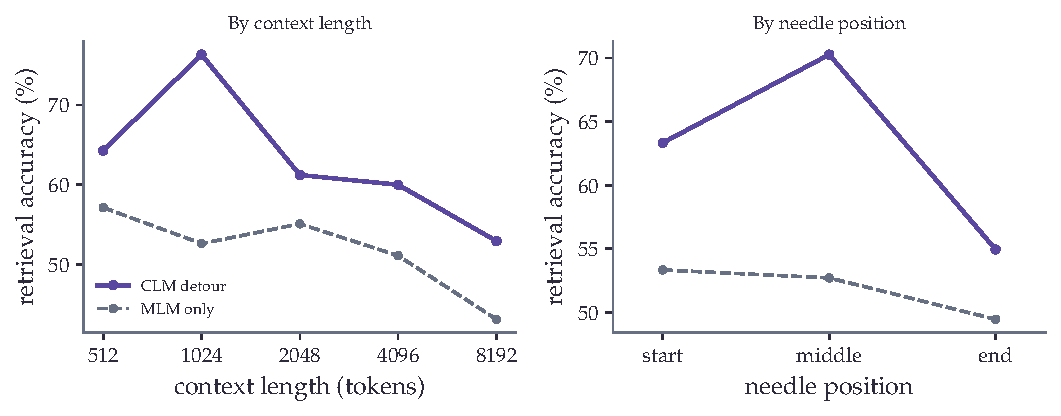
\includegraphics[width=\textwidth]{plots/chapter5/needle.pdf}
  \caption{Needle-in-a-haystack retrieval in French, binary accuracy of a frozen-encoder
  probe. The CLM detour stays above the MLM-only model at every context length (left) and
  at every needle position (right), with the largest margin at mid-document.}
  \label{fig:needle}
\end{figure}

\begin{reviewread}
Long-context encoding is critical in biomedical NLP, where clinical documents routinely span thousands of tokens and key information (diagnoses, coding labels) can appear anywhere in the document. We design a synthetic needle-in-a-haystack task in French to evaluate long-context retrieval without entity-type confounds.
\end{reviewread}

\paragraph{Protocol.} A medical fact (the ``needle'') is inserted into a clinical document (the ``haystack'') at a controlled position, and the model must determine whether a given query fact is present (binary classification). Negative examples use the same template with different slot values, so the task requires precise retrieval rather than shallow pattern matching. We define 8 French medical fact templates covering drugs, vital signs, lab results, diagnoses, procedures, allergies, treatment duration, and symptoms. Each template has 2--4 slots filled from small lexicons:

\begin{itemize}
  \item \textit{Le patient a re\c{c}u 200\,mg de morphine par voie intraveineuse.}\\
        \textbf{Distractor:} \textit{Le patient a re\c{c}u 500\,mg de tramadol par voie orale.}
  \item \textit{La tension art\'erielle mesur\'ee \'etait de 160/90\,mmHg.}
  \item \textit{Le diagnostic retenu est cirrhose h\'epatique de stade~III.}
  \item \textit{Le patient rapporte une dyspn\'ee \'evoluant depuis une semaine.}
\end{itemize}

\begin{reviewread}
We generate 1,500 balanced positive/negative pairs across 5 lengths (512--8,192 tokens) and 3 positions (start, middle, end), split 70/15/15 for train/validation/test. We freeze each encoder and train a 2-layer MLP probe (Dropout $\to$ Linear $\to$ GELU $\to$ Dropout $\to$ Linear) on CLS representations for 3 epochs (lr $= 2 \times 10^{-5}$, batch size 4, AdamW), selecting the best checkpoint by validation accuracy.
\end{reviewread}

\paragraph{Results.} CLM outperforms MLM at every context length and position (\Cref{fig:needle}; +10.7pp overall: 62.2\% vs 51.6\%). MLM accuracy degrades monotonically with document length (57\% at 512 tokens to 43\% at 8,192), while CLM degrades more slowly and remains above MLM throughout. The CLM advantage is largest at mid-document positions, where the inserted fact is farthest from both sequence boundaries. This is consistent with the downstream pattern: the French tasks with the largest CLM gains (FrACCO, CANTEMIST) use sequence lengths of 4,096 tokens during fine-tuning.


\section{Analysis: Why Does the CLM Detour Work?}
\label{sec:analysis}

\subsection{CKA Methodology}
\label{sec:cka_method}

We measure representational similarity with linear Centered Kernel Alignment~\citep{kornblith2019similarity}. Given two representation matrices $X \in \mathbb{R}^{n \times p}$ and $Y \in \mathbb{R}^{n \times q}$ (one per model, $n$ samples, mean-pooled over tokens), we center each column, compute Gram matrices $K = XX^\top$ and $L = YY^\top$, and define:
\[
\text{CKA}(X, Y) = \frac{\text{tr}(KL)}{\sqrt{\text{tr}(K^2)\,\text{tr}(L^2)}}
\]
We report divergence $d = 1 - \text{CKA}$, so higher values indicate greater representational difference. CKA equals 1 when representations are identical up to invertible linear transformation, 0 when there is no linear relationship. All computations use float64 arithmetic. For French we use 500 held-out texts from DiaMED and FrACCO; for English, PubMed abstracts. Results are averaged over 3 seeds.

\subsection{The CLM Imprint Persists in Low Layers}
\label{sec:persistence}

\begin{figure}[t]
  \centering
  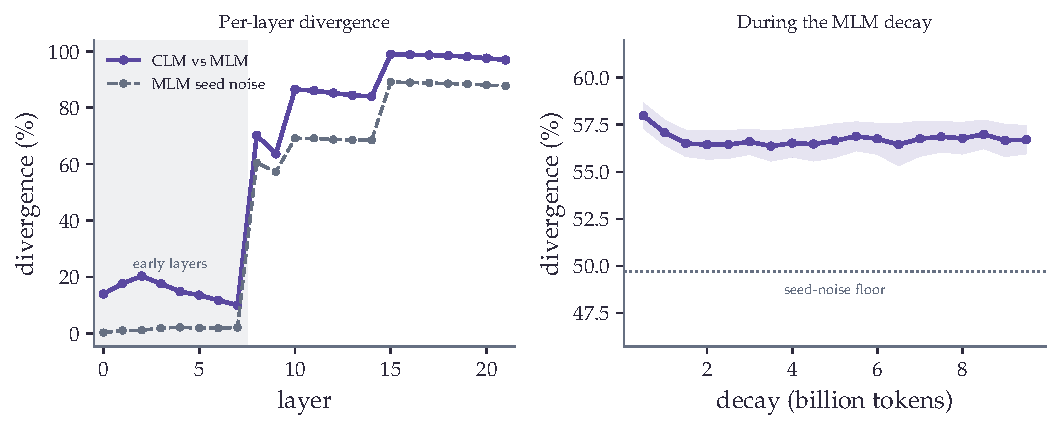
\includegraphics[width=\textwidth]{plots/chapter5/cka_mechanism.pdf}
  \caption{Where the detour leaves its mark, measured by representational divergence
  ($1-\text{CKA}$, held-out clinical text, three seeds). Left: per layer, the CLM-vs-MLM
  pair against a same-objective seed-noise control; the early layers diverge several times
  more than the noise floor. Right: during the MLM decay the divergence plateaus well above
  the seed-noise floor, so decaying back to masked training does not return the model to an
  MLM-like state.}
  \label{fig:cka-mechanism}
\end{figure}

\begin{reviewread}
Comparing layer-by-layer CKA between CLM-detour and MLM-only models (\Cref{fig:cka-mechanism}), the CLM phase modifies low-layer representations in a way that subsequent MLM training does not undo, even when the decay budget matches the CLM phase. CKA divergence reaches approximately 56.5\% after 1.5B tokens of MLM decay and remains stable, with only 0.6pp variation over 8B additional tokens.
\end{reviewread}

To isolate where CLM differs from MLM \emph{specifically} rather than just from training noise, we normalize each layer's CLM-MLM divergence by a seed-noise control (two MLM models trained with different random seeds on identical data):
\[
r_\ell = \frac{1 - \text{CKA}(\text{CLM}_\ell,\; \text{MLM}^{s_1}_\ell)}{1 - \text{CKA}(\text{MLM}^{s_2}_\ell,\; \text{MLM}^{s_1}_\ell)}
\]
A ratio of 1 means no CLM-specific effect. Low layers (0--7) show ratios of 5--44$\times$: CLM changes them far more than random seed variation does. Mid and deep layers are near 1$\times$: both objectives modify them similarly, so CKA cannot distinguish CLM from MLM there.

\subsection{Causal Evidence: Freeze Interventions}
\label{sec:freeze-results}

\begin{figure}[t]
  \centering
  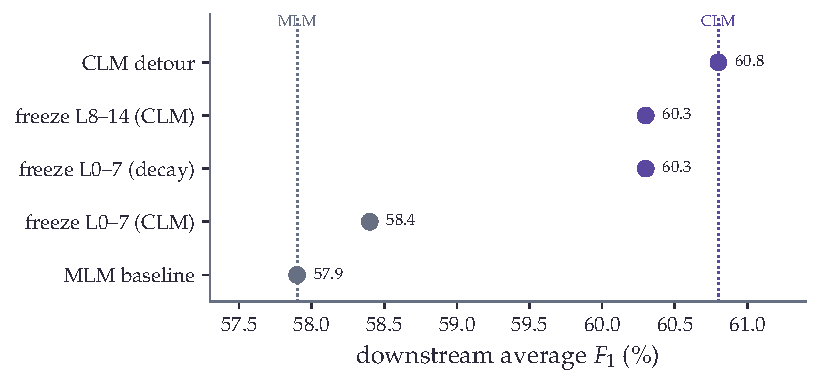
\includegraphics[width=0.8\textwidth]{plots/chapter5/freeze.pdf}
  \caption{Freeze interventions (French Base, 8 tasks, 9 seeds). Freezing the low
  layers during the CLM phase drops the model back onto the MLM baseline, while
  freezing the mid layers, or freezing the low layers during the decay, keeps the
  full gain: the low layers are necessary during the causal phase, the mid layers
  are not.}
  \label{fig:freeze}
\end{figure}

\begin{reviewread}
Do these low-layer changes actually drive the downstream improvement? A freeze experiment holds a group of layers fixed during one phase of training, so that the rest of the model still trains normally around it. If the benefit depends on a layer group being modified during a given phase, freezing that group in that phase should remove the benefit. We run three such experiments on the 22-layer French Base model, where the CLM-MLM gap is largest (+2.9pp):
\end{reviewread}

\begin{itemize}
    \item \textbf{Experiment~1} (low freeze, CLM phase): Layers 0--7 frozen during CLM, then normal decay. Tests whether low-layer modification during CLM is necessary.
    \item \textbf{Experiment~2} (low freeze, decay phase): Normal CLM, then layers 0--7 frozen during decay. Tests whether low-layer CLM changes persist without further updates.
    \item \textbf{Experiment~3} (mid freeze, CLM phase): Layers 8--14 frozen during CLM, then normal decay. Together with Experiment~1, tests selectivity: if freezing low layers eliminates the benefit while freezing mid layers preserves it, this constitutes a double dissociation.
\end{itemize}

\begin{reviewread}
The three conditions are summarized in \Cref{fig:freeze} and \Cref{tab:freeze}.
\end{reviewread}

\begin{table}[t]
\centering
\small
\begin{tabular}{lcc}
\toprule
\textbf{Condition} & \textbf{Avg $F_1$} & $\boldsymbol{\Delta}$ \textbf{vs MLM} \\
\midrule
\rowcolor{ThesisTableSep} \multicolumn{3}{c}{\rule{0pt}{9pt}\textbf{References}} \\[1pt]
MLM baseline & 57.9 & --- \\
CLM detour & \bfseries 60.8 & +2.9 \\
\midrule
\rowcolor{ThesisTableSep} \multicolumn{3}{c}{\rule{0pt}{9pt}\textbf{Freeze interventions}} \\[1pt]
Freeze L0--7 (CLM phase) & 58.4 & +0.5 \\
Freeze L8--14 (CLM phase) & 60.3 & +2.4 \\
Freeze L0--7 (decay phase) & 60.3 & +2.4 \\
\bottomrule
\end{tabular}
\caption{\textbf{Freeze intervention results} (French Base, 8 tasks, 9 seeds). Freezing low layers during CLM eliminates the benefit ($p=0.36$ vs MLM baseline). Freezing mid layers preserves it. Freezing low layers during decay has negligible effect.}
\label{tab:freeze}
\end{table}

\begin{reviewread}
Freezing low layers (0--7) during CLM drops $F_1$ from 60.8\% to 58.4\%. We cannot reject the null hypothesis that the resulting model matches the MLM baseline ($p = 0.36$, paired bootstrap across 8 tasks $\times$ 9 seeds). Freezing mid layers (8--14) during CLM preserves the full benefit (60.3\%). Together, these two experiments establish a double dissociation: low layers are necessary and mid layers are not. Freezing low layers during decay has negligible effect ($-$0.5pp, 60.3\%), confirming that MLM decay preserves the CLM imprint in low layers.
\end{reviewread}

\subsection{Non-Localizability}

\begin{reviewread}
The freeze experiments show that low layers are necessary \emph{during training}. We now ask whether the resulting benefit can be localized \emph{after training}, by copying full parameter blocks from the CLM model into the MLM model.
\end{reviewread}

\begin{table}[t]
\centering
\small
\begin{tabular}{lccc}
\toprule
\textbf{Transplant} & \textbf{$F_1$ (\%)} & $\boldsymbol{\Delta}$ & \textbf{Recovery} \\
\midrule
\rowcolor{ThesisTableSep} \multicolumn{4}{c}{\rule{0pt}{9pt}\textbf{References}} \\[1pt]
MLM baseline & 32.8 & --- & 0\% \\
CLM detour & 39.9 & +7.1 & 100\% \\
\midrule
\rowcolor{ThesisTableSep} \multicolumn{4}{c}{\rule{0pt}{9pt}\textbf{Layer group transplants}} \\[1pt]
Low (0--7) & 31.9 & $-$0.9 & $-$12\% \\
Mid (8--14) & 35.3 & +2.5 & +35\% \\
Late (15--21) & 32.4 & $-$0.4 & $-$6\% \\
\bottomrule
\end{tabular}
\caption{\textbf{Layer transplantation} on DiaMED (3 seeds, linear probing). All transplants recover at most 35\% of the 7.1pp gap.}
\label{tab:transplant}
\end{table}

\begin{reviewread}
No transplant recovers more than 35\% of the gap (\Cref{tab:transplant}). Low and late layer transplants hurt performance. Inserting CLM low layers into an MLM model creates a mismatch with the mid and deep layers that co-adapted under MLM, yielding representations worse than either pure model.
\end{reviewread}

\begin{reviewread}
Component-level transplants (\Cref{tab:transplant-comp}) confirm the same pattern. Replacing all attention modules from CLM into MLM recovers only 15\% of the gap; replacing all MLP blocks recovers 35\%. No single component type captures the full benefit.
\end{reviewread}

\begin{table}[t]
\centering
\small
\begin{tabular}{lccc}
\toprule
\textbf{Transplant} & \textbf{$F_1$ (\%)} & $\boldsymbol{\Delta}$ & \textbf{Recovery} \\
\midrule
All attention & 33.9 & +1.1 & +15\% \\
All MLP & 35.3 & +2.5 & +35\% \\
\bottomrule
\end{tabular}
\caption{\textbf{Component-level transplants} on DiaMED (3 seeds, linear probing). Neither attention nor MLP modules alone recover the full gap.}
\label{tab:transplant-comp}
\end{table}

\begin{reviewread}
Unlike freeze interventions, which act during training, transplants replace already-trained weights and cannot reconstruct the cross-layer co-adaptation that developed during CLM. The freeze experiments show low layers are necessary during training; the transplant experiments show the resulting benefit cannot be isolated post hoc.
\end{reviewread}

\subsection{Scaling and Architectural Asymmetry}
\label{sec:asymmetry}

\begin{table}[t]
\centering
\small
\begin{tabular}{llcc}
\toprule
\textbf{Model} & \textbf{Params} & \textbf{Div.} & \textbf{CI} \\
\midrule
\rowcolor{ThesisTableSep} \multicolumn{4}{c}{\rule{0pt}{9pt}\textbf{Encoders (MLM$\to$CLM$\to$MLM)}} \\[1pt]
ModernCamemBERT Base & 150M & 56.5\% & $\pm$0.7\% \\
ModernCamemBERT Large & 350M & 67.2\% & $\pm$0.3\% \\
\midrule
\rowcolor{ThesisTableSep} \multicolumn{4}{c}{\rule{0pt}{9pt}\textbf{Decoder (CLM$\to$MLM$\to$CLM)}} \\[1pt]
Gemma-3 & 270M & 26.3\% & $\pm$1.0\% \\
\bottomrule
\end{tabular}
\caption{\textbf{CKA divergence scales with model size and is asymmetric.} The encoder-decoder comparison uses different model families (see text).}
\label{tab:asymmetry}
\end{table}

\begin{reviewread}
The CLM imprint increases with model capacity (\Cref{tab:asymmetry}): Large (350M) reaches 67.2\% $\pm$ 0.3\% divergence versus 56.5\% $\pm$ 0.7\% for Base (150M). Testing the reverse on Gemma-3 (270M decoder), MLM-then-CLM retains only 26.3\% $\pm$ 1.0\% divergence versus 67.2\% for an encoder of similar scale. One explanation is the density of the decay signal: MLM decay at 15\% masking provides weak erasure, while CLM decay at 100\% provides strong erasure. This comparison is exploratory: it is confounded by model family and language, and a controlled comparison using encoder and decoder variants of the same family would be needed to confirm the asymmetry.
\end{reviewread}


\section{Limitations}

\begin{reviewread}
Our freeze interventions use French Base models only. The CKA patterns that motivate them (low-layer divergence well above seed noise) are consistent across French Base, French Large, and English Base, but replication of the freeze interventions on English and Large models would strengthen the causal claim. The encoder-decoder asymmetry comparison is confounded by model family. The position trade-off at 2048+ tokens means that the approach may not be suitable for tasks requiring very long context, such as full discharge summary coding.
\end{reviewread}


\section*{Conclusion}

\begin{reviewread}
Training an encoder like a decoder, then converting it back, produces stronger representations than training with MLM alone. The CLM detour reshapes low transformer layers in ways that subsequent MLM decay does not undo: a lasting imprint that scales with model capacity and produces consistent downstream gains across 8 French and 11 English biomedical tasks.
\end{reviewread}

\begin{reviewread}
For biomedical encoder pretraining, the CLM detour improves results at no extra cost, using the same data and the same compute budget as MLM-only pretraining. MLM decay of roughly 10\% of the detour length suffices, and the effect is strongest when the domain gap between pretraining and target data is large.
\end{reviewread}

\vspace{2em}

\begin{reviewread}
Parts~1 and 2 of this thesis have focused on data and pretraining: how to collect biomedical text, how to filter it, and how to train encoder models on it. But a pretrained model is only useful if it can be deployed on real tasks. In the next part, we turn to adaptation: how to extract clinical information when labeled data is scarce, labels number in the thousands, and the only available text is public.
\end{reviewread}


\chapter{Knowledge-Enriched Pretraining}
\label{chap:ontobook}
% This chapter is based on:
%   Rian Touchent, Éric de La Clergerie.
%   OntoBook: Ontology-Grounded Synthetic Textbooks for Medical Encoder Pretraining.
%   LREC 2026.
%
% Source: publications/OntoBook/
% Sections concatenated verbatim from the paper:
%   introduction.tex, related.tex, method.tex, experiments.tex, discussion.tex
% TODO: adapt tables and figures to thesis-style.sty (visual-style.md)
% TODO: rewrite intro as a thesis-contextualized hook (not the paper's intro)
% TODO: integrate \Cref{} cross-references to other chapters

% Local macro for OntoBook (matches publications/OntoBook/main.tex)
\providecommand{\method}{OntoBook\xspace}

\begin{figure}[t]
\centering
\begin{tikzpicture}[scale=0.78, transform shape,
  stage/.style={font=\scriptsize\sffamily\bfseries, text=#1},
  frame/.style={rounded corners=5pt, draw=ThesisNeutral!40, minimum height=2.6cm},
]

  % === THREE FRAMES ===
  \node[frame, minimum width=2.5cm]  (f1) at (1.25, 1.0) {};
  \node[frame, minimum width=5.0cm]  (f2) at (6.5,  1.0) {};
  \node[frame, minimum width=4.5cm]  (f3) at (12.75,1.0) {};

  % === STAGE LABELS ===
  \node[stage=ThesisPrimaryDark]   at (f1.north) [above=2pt] {Ontology};
  \node[stage=ThesisSecondaryDark] at (f2.north) [above=2pt] {Textbook {\scriptsize(1.3B tokens)}};
  \node[stage=ThesisTertiaryDark]  at (f3.north) [above=2pt] {Aligned training};

  % === F1: mini ontology graph ===
  \node[rectangle, rounded corners=3pt, draw=ThesisPrimaryDark, fill=ThesisPrimary!15, inner sep=2.5pt,
        font=\scriptsize\ttfamily, minimum width=0.7cm] (e11) at ([xshift=-8mm,yshift=5mm]f1.center) {E11};
  \node[rectangle, rounded corners=3pt, draw=ThesisPrimaryDark, fill=ThesisPrimary!15, inner sep=2.5pt,
        font=\scriptsize\ttfamily, minimum width=0.7cm] (n08) at ([xshift=7mm,yshift=5mm]f1.center) {N08};
  \node[rectangle, rounded corners=3pt, draw=ThesisPrimaryDark, fill=ThesisPrimary!15, inner sep=2.5pt,
        font=\scriptsize\ttfamily, minimum width=0.7cm] (n083) at ([xshift=7mm,yshift=-5mm]f1.center) {N08.3};
  \draw[-{Stealth[length=1.5mm]}, ThesisPrimary!70, thick]
    (e11) -- node[above=-1pt, font=\tiny\sffamily, text=ThesisInk] {\textsc{causes}} (n08);
  \draw[-{Stealth[length=1.5mm]}, ThesisPrimary!70, thick]
    (n08) -- node[left=-1pt, font=\tiny\sffamily, text=ThesisInk] {\textsc{parent}} (n083);

  % === F2: textbook paragraph ===
  \node[draw=ThesisSecondaryDark, fill=ThesisSecondary!10, rounded corners=3pt,
        text width=4.4cm, font=\scriptsize, inner sep=4pt, align=justify] (para) at (f2.center)
    {Le diab\`ete (\textcolor{ThesisPrimaryDark}{\textbf{E11}}) peut entra\^iner
     une glom\'erulopathie (\textcolor{ThesisPrimaryDark}{\textbf{N08}}),
     notamment la forme diab\'etique (\textcolor{ThesisPrimaryDark}{\textbf{N08.3}})\ldots};

  % === F3: two objectives ===
  \node[draw=ThesisTertiaryDark, fill=ThesisTertiary!15, rounded corners=2pt,
        text width=3.6cm, font=\scriptsize, inner sep=4pt] (mlmex) at ([yshift=5.2mm]f3.center)
    {$\mathcal{L}_{\text{MLM}}$:\; Le \colorbox{ThesisTertiary!30}{[MASK]} (E11) peut
     \colorbox{ThesisTertiary!30}{[MASK]} une n\'ephropathie\ldots};
  \node[draw=ThesisTertiaryDark, fill=ThesisTertiary!15, rounded corners=2pt,
        text width=3.6cm, font=\scriptsize, inner sep=4pt] (relex) at ([yshift=-6.8mm]f3.center)
    {$\mathcal{L}_{\text{rel}}$:\qquad E11 $\xrightarrow{\;\colorbox{ThesisTertiary!30}{\textbf{?}}\;}$ N08};

  % === ARROWS ===
  \draw[-{Stealth[length=2.5mm]}, line width=1.2pt, draw=ThesisNeutral]
    (f1.east) -- node[above, font=\tiny\sffamily, text=ThesisInk] {Qwen3-235B} (f2.west);
  \draw[-{Stealth[length=2mm]}, line width=1pt, draw=ThesisNeutral]
    (f2.east) -- node[above, font=\tiny\sffamily, text=ThesisInk] {Multi-task} (f3.west);

\end{tikzpicture}
\caption{\textbf{\method pipeline.} An ontology subgraph is converted into a random walk, then reformulated into textbook prose by Qwen3-235B. The encoder trains on this text with two aligned objectives: masked language modeling and relation prediction between code pairs.}
\label{fig:ontobook-pipeline}
\end{figure}

\section{Introduction}
\label{sec:intro}

Medical coding is the task of assigning standardized codes from medical ontologies to clinical documents. It is central to hospital billing, epidemiological surveillance, and clinical research. In France, over 30 million hospital stays per year require accurate coding using the CIM-10 classification (the French adaptation of ICD-10), CCAM procedure codes, and ATC medication codes. This task requires understanding not only medical vocabulary but also the relational structure of medical ontologies: hierarchical links between codes, causal associations, differential diagnoses, and exclusion rules. These relationships are explicitly encoded in ontology graphs but are absent from clinical text corpora.

Pretrained biomedical language models such as BioBERT \citep{lee2020biobert}, PubMedBERT \citep{gu2021pubmedbert}, and CamemBERT-bio \citep{touchent2023camembertbio} learn medical vocabulary from large text corpora. However, they do not capture the relational structure of medical ontologies, since this structure is not expressed in running text. Knowledge graph approaches such as RDF2Vec \citep{ristoski2016rdf2vec} and Snomed2Vec \citep{agarwal2019snomed2vec} encode ontology structure through random walks, but produce static, non-contextualized embeddings that cannot benefit from transformer pretraining. Knowledge-enhanced transformers such as DRAGON \citep{yasunaga2022dragon} and KEPLER \citep{wang2021kepler} integrate knowledge graph structure into language model pretraining, but they rely on existing text-graph alignment rather than generating new training data from ontology structure alone.

We propose \method, a pretraining method that converts medical ontology structure into training signal for encoder language models. Our approach proceeds in three stages. First, we generate random walks through ontology graphs to produce sequences that capture hierarchical, causal, and differential relationships between medical codes. Second, we reformulate these walks into fluent medical prose using a large language model, creating synthetic textbooks grounded in ontology structure. Third, we train an encoder with two objectives on the same textbook data: masked language modeling and relation prediction between code pairs. We refer to this co-training on shared data as \emph{alignment}, and our experiments show that it is a necessary condition for the method to work.

We evaluate \method on three French medical coding benchmarks and present ablation studies on the contribution of each component. We release 1.3 million LLM-reformulated medical textbooks across three French ontologies (CIM-10, CCAM, ATC) and all pretrained model checkpoints.
\section{Related Work}
\label{sec:related}

This section reviews three research directions: biomedical language model pretraining, knowledge-enhanced language models, and automatic medical coding.

\subsection{Biomedical Pretrained Language Models}

Domain-specific pretraining has proven essential for biomedical NLP. BioBERT \citep{lee2020biobert} further pretrained BERT on PubMed abstracts and PMC full-text articles, improving named entity recognition and relation extraction. PubMedBERT \citep{gu2021pubmedbert} demonstrated that pretraining from scratch on in-domain text outperforms mixed-domain initialization. ClinicalBERT \citep{huang2019clinicalbert} targeted clinical notes from MIMIC-III. For French, CamemBERT-bio \citep{touchent2023camembertbio} adapted CamemBERT \citep{martin2020camembert} to biomedical text, while DrBERT \citep{labrak2023drbert} was trained on French biomedical and clinical text from the NACHOS corpus. These models learn from flat text corpora and do not capture the hierarchical structure of medical ontologies.

\subsection{Knowledge-Enhanced Language Models}

Random walks on knowledge graphs generate sequences capturing relational structure. RDF2Vec \citep{ristoski2016rdf2vec} adapted the walk-then-embed paradigm to RDF graphs. In the biomedical domain, Snomed2Vec \citep{agarwal2019snomed2vec} applied random walk and Poincar\'e embeddings to SNOMED-CT for clinical prediction tasks. OWL2Vec* \citep{chen2021owl2vec} combined random walk sequences with lexical and logical features from OWL ontologies. These methods produce static embeddings (Word2Vec-style) and cannot be used for transformer pretraining.

Several approaches inject knowledge graph structure into transformers. ERNIE \citep{zhang2019ernie} aligns entity embeddings with text representations. K-BERT \citep{liu2020kbert} injects knowledge triples into the input sequence using soft-position indices and a visibility mask. For multi-task pretraining, KEPLER \citep{wang2021kepler} combines MLM with TransE-style knowledge embedding on Wikidata. DRAGON \citep{yasunaga2022dragon} jointly trains MLM and knowledge graph link prediction, with a biomedical variant on UMLS achieving +3\% on MedQA. CODER \citep{yuan2021coder} uses UMLS relation triplets for contrastive pretraining, and SAPBERT \citep{liu2021sapbert} uses contrastive learning on UMLS synonyms for biomedical entity linking. Closest to the present work, BioOntoBERT \citep{shashikumar2023bioontobert} generates sentences from biomedical ontologies using Onto2Sen templates and pretrains BERT with MLM on the resulting corpus. However, the template-based generation produces formulaic sentences (e.g., ``X is a type of Y'') rather than fluent prose, and the method uses only MLM without multi-task relation prediction.

Recent work has explored synthetic data generation from knowledge sources. The Phi series \citep{gunasekar2023phi} demonstrated that LLM-generated textbook-quality data enables strong small-model performance. EntiGraph \citep{yang2025entigraph} generates entity-centric synthetic data from knowledge sources but targets decoder language models rather than encoder pretraining.

\subsection{Automatic Medical Coding}

Medical coding assigns ICD, procedure, or medication codes to clinical text. CAML \citep{mullenbach2018explainable} introduced label-wise attention for explainable predictions. PLM-ICD \citep{huang2022plmicd} showed that fine-tuning pretrained encoders with label attention directly improves coding performance. \citet{kirchler2026grasp} recently demonstrated that LLM embeddings improve transferability of EHR-based predictions across countries and coding systems, highlighting the importance of encoding medical knowledge structure for cross-system generalization. These methods improve the classification head or the input representations but rely on generic encoders pretrained on flat text corpora.

Table~\ref{tab:related_comparison} summarizes how \method combines components not jointly present in prior work.

\begin{table}[t]
\centering
\small
\setlength{\tabcolsep}{8pt}
\begin{tabular}{lccc}
\toprule
\textbf{Method} & \textbf{Walks} & \textbf{LLM} & \textbf{MLM+Rel} \\
\midrule
\rowcolor{ThesisTableSep}
\multicolumn{4}{c}{\rule{0pt}{10pt}\textbf{Prior work}} \\[1pt]
Snomed2Vec & \checkmark & & \\
BioOntoBERT & \checkmark & & \\
DRAGON & & & \checkmark \\
KEPLER & & & \checkmark \\
Phi-1 & & \checkmark & \\
\midrule
\rowcolor{ThesisTableSep}
\multicolumn{4}{c}{\rule{0pt}{10pt}\textbf{Ours}} \\[1pt]
\textbf{\method} & \checkmark & \checkmark & \checkmark \\
\bottomrule
\end{tabular}
\caption{\textbf{Comparison with related approaches.} \method uniquely combines all three components for biomedical encoder pretraining.}
\label{tab:related_comparison}
\end{table}
\section{Method}
\label{sec:method}

\method converts medical ontology structure into pretraining signal through three stages: (1) generating random walks through ontology graphs, (2) reformulating these walks into fluent textbook prose using a large language model, and (3) training an encoder with multi-task learning combining masked language modeling and relation prediction. We first describe the ontologies used, then detail each stage. Figure~\ref{fig:ontobook-pipeline} illustrates the full pipeline.

\subsection{Medical Ontologies}
\label{sec:ontologies}

We use three French medical ontologies published by the Agence du Num\'erique en Sant\'e (ANS) through its terminology server (SMT) in RDF/OWL format. CIM-10 FR PMSI is the French adaptation of the WHO's ICD-10, enriched by the Agence Technique de l'Information sur l'Hospitalisation (ATIH) for the French hospital information system (Programme de M\'edicalisation des Syst\`emes d'Information, PMSI). It contains 19,161 diagnostic codes organized in a 5-level hierarchy (chapters, blocks, categories, subcategories), with textual annotations including 23,282 synonyms, 8,171 inclusion notes, and 381 definitions. CIM-10 is the only ontology with semantic edges beyond the hierarchy: 1,317 causal edges (e.g., E11 type 2 diabetes \textit{causes} N08.3 diabetic glomerulopathy), 5,739 exclusion edges, and 341 manifestation edges, yielding a mean node degree of 2.77 compared to 2.00 for the purely hierarchical ontologies.

CCAM (Classification Commune des Actes M\'edicaux) is the French procedure classification maintained by the Caisse Nationale d'Assurance Maladie (CNAM), containing 38,191 procedure codes in a 4-level hierarchy with 8,991 synonyms and 1,188 disjointness constraints between mutually exclusive procedures. ATC (Anatomical Therapeutic Chemical) is the WHO medication classification with 6,950 substance codes in a strict 5-level hierarchy from anatomical group to chemical substance, with no semantic edges, no synonyms, and no definitions beyond labels. This contrast in relational richness directly shapes the walk generation strategy: CIM-10 walks can follow causal and differential diagnosis paths, whereas CCAM and ATC walks are limited to hierarchical and sibling traversals. Table~\ref{tab:ontology_stats} summarizes the structural properties of the three ontologies.

\begin{table}[t]
\centering
\small
\begin{tabular}{lrrr}
\toprule
& \textbf{CIM-10} & \textbf{CCAM} & \textbf{ATC} \\
\midrule
\rowcolor{ThesisTableSep}
\multicolumn{4}{c}{\rule{0pt}{10pt}\textbf{Graph structure}} \\[1pt]
Codes & 19,161 & 38,191 & 6,950 \\
Hierarchy depth & 5 & 4 & 5 \\
Hierarchical edges & 19,139 & 38,191 & 6,950 \\
Causal edges & 1,317 & --- & --- \\
Manifestation edges & 341 & --- & --- \\
Exclusion edges & 5,739 & --- & --- \\
Disjoint edges & --- & 1,188 & --- \\
Mean degree & 2.77 & 2.06 & 2.00 \\
\midrule
\rowcolor{ThesisTableSep}
\multicolumn{4}{c}{\rule{0pt}{10pt}\textbf{Textual attributes}} \\[1pt]
Synonyms & 23,282 & 8,991 & 0 \\
Inclusion notes & 8,171 & --- & --- \\
Definitions & 381 & 151 & 0 \\
\bottomrule
\end{tabular}
\caption{\textbf{Structural properties} of the three French medical ontologies used for walk generation. CIM-10 is the only ontology with semantic edges beyond the hierarchy.}
\label{tab:ontology_stats}
\end{table}

\subsection{Ontology Walk Generation}
\label{sec:walks}

We generate random walks through ontology graphs to capture relational structure in a sequential format suitable for language model pretraining. We sample walks starting from each code in the ontology. At each step, the next node is selected via weighted sampling where edge type weights depend on the walk type. This biased sampling is necessary because semantic edges are rare (Table~\ref{tab:ontology_stats}), and a uniform walk would rarely traverse them. Each walk records the traversed codes along with their labels and the relation types connecting them. Walk length is sampled uniformly between 8 and 20 steps. We track visited nodes to avoid cycles, with a fallback that allows revisiting nodes when all neighbors have been explored.

For CIM-10, we define five walk types, each emphasizing different aspects of medical knowledge: \textit{Etiologie} (causal chains), \textit{Diagnostic Diff\'erentiel} (codes to distinguish clinically), \textit{Codage Double} (mandatory code pairs linking etiology to manifestation), \textit{Syndrome} (multi-system manifestations), and \textit{Cross-Chapter} (connections between different ICD chapters, e.g., diabetes E11 to its renal complication N08). We generate 402,328 walks for CIM-10 (average 4,830 characters), 762,958 for CCAM, and 138,980 for ATC, totaling 1,304,266 walks.

\subsection{Textbook Generation}
\label{sec:textbook}

Raw walks contain structured markers (e.g., ``\texttt{>> \`A distinguer de:}'') that are useful for parsing but not natural for language model pretraining. We use a large language model to reformulate walks into fluent medical prose resembling textbook paragraphs.

We prompt Qwen3-235B-A22B-Instruct \citep{yang2025qwen3} with FP8 quantization to transform each walk into a coherent paragraph. The prompt instructs the model to: (1) preserve all medical codes and their relationships exactly as stated, (2) use natural medical language without lists or bullet points, (3) not add any information beyond what appears in the walk. This ensures the textbook content remains grounded in the ontology structure. We apply two filters: we discard reformulations shorter than 50 characters or that fail to mention the source codes. The reformulation runs on 4 NVIDIA H100 GPUs using vLLM \citep{kwon2023vllm} with guided decoding to ensure valid JSON output, taking approximately 20 hours for all 1.3 million walks. The resulting textbooks contain approximately 1.3 billion tokens across all three ontologies. Figure~\ref{fig:textbook_example} shows an example transformation.

\begin{figure}[t]
\centering
\begin{tikzpicture}[node distance=0.3cm]
  \node[draw=ThesisPrimaryDark, fill=ThesisPrimary!10, rounded corners=3pt,
        text width=6.5cm, align=left, inner sep=6pt,
        font=\scriptsize\ttfamily] (walk) {
    \textcolor{ThesisPrimaryDark}{\textbf{[F02.0]}} D\'emence de la maladie de Pick\\[2pt]
    \textcolor{ThesisNeutral}{>>} Cette pathologie peut provoquer:\\
    \textcolor{ThesisPrimaryDark}{\textbf{[G31.0]}} Atrophie c\'er\'ebrale circonscrite\\[2pt]
    \textcolor{ThesisNeutral}{>>} Parmi les causes possibles:\\
    \textcolor{ThesisPrimaryDark}{\textbf{[F02.02]}} ...avec sympt\^omes hallucinatoires
  };
  \node[above=0.1cm of walk, font=\scriptsize\sffamily\bfseries, text=ThesisPrimaryDark] {Structured Walk};
  \node[below=0.4cm of walk, font=\small] (arrow) {$\downarrow$ \textit{Qwen3-235B}};
  \node[draw=ThesisSecondaryDark, fill=ThesisSecondary!10, rounded corners=3pt,
        text width=6.5cm, align=justify, inner sep=6pt,
        font=\scriptsize, below=0.4cm of arrow] (textbook) {
    Le code \textcolor{ThesisSecondaryDark}{\textbf{F02.0}}, d\'esignant la d\'emence de la maladie de Pick,
    s'inscrit dans un r\'eseau de connexions inter-syst\`emes entre les troubles mentaux et les
    affections neurologiques. Ce code entretient une relation \'etroite avec
    \textcolor{ThesisSecondaryDark}{\textbf{G31.0}} (atrophie c\'er\'ebrale circonscrite), \'etablissant
    un lien \'etiologique r\'eciproque...
  };
  \node[above=0.1cm of textbook, font=\scriptsize\sffamily\bfseries, text=ThesisSecondaryDark] {Medical Textbook};
\end{tikzpicture}
\caption{\textbf{Walk-to-textbook transformation.} The structured walk is reformulated into fluent medical prose while preserving all codes and relations.}
\label{fig:textbook_example}
\end{figure}

Figure~\ref{fig:prompt} shows the system prompt used for CIM-10 walks (translated from French for readability; prompts for CCAM and ATC follow the same structure with ontology-specific terminology).

\begin{figure}[t]
\centering
\begin{tikzpicture}
\node[draw=ThesisNeutral, fill=ThesisPaper, rounded corners=4pt,
      text width=0.9\columnwidth, inner sep=10pt, font=\scriptsize, align=left] {%
\textbf{\sffamily Reformulation Prompt (CIM-10, translated)}\\[6pt]
You are an expert medical writer specializing in high-quality educational material.\\[3pt]
Reformulate the provided CIM-10 walk into fluent, textbook-quality medical prose.\\[3pt]
\textbf{Strict rules:}\\
(1) \textbf{No invention}: never add information not in the source.\\
(2) \textbf{Total fidelity}: preserve all definitions, codes, clinical notes, exclusions.\\
(3) \textbf{Completeness}: do not omit any source information.\\
(4) \textbf{Ignore metadata}: never mention walk types or structural headers.\\[3pt]
\textbf{Style:} Continuous narrative prose, no bullet points or markdown. Integrate CIM-10 codes naturally. Preserve exact medical terminology.\\[3pt]
\textbf{Goal:} Transform the walk into text suitable for a medical nosology textbook chapter while remaining 100\% faithful to the original content.%
};
\end{tikzpicture}
\caption{System prompt for LLM-based walk reformulation. Temperature is set to 0 for deterministic, faithful output.}
\label{fig:prompt}
\end{figure}

\subsection{\method Training}
\label{sec:training}

We train a ModernCamemBERT-base encoder \citep{music2025moderncamembert}, initialized from a French checkpoint trained on 1 trillion tokens.

The model optimizes two objectives jointly. The first, $\mathcal{L}_{\text{MLM}}$, follows standard masked language modeling \citep{devlin2019bert}: we mask 15\% of tokens from textbook paragraphs and train to predict them. The second, $\mathcal{L}_{\text{rel}}$, classifies the relationship between pairs of medical codes. Our main model uses CIM-10; we explore transfer from CCAM and ATC in Section~\ref{sec:multi_onto}. We extract 282,907 code pairs from the CIM-10 ontology across 6 relation types: \textsc{Parent}, \textsc{Child}, \textsc{Sibling}, \textsc{Differential Diagnosis}, \textsc{Causes}, and \textsc{Caused\_By}. For each pair, we retrieve the corresponding textbook descriptions generated in Section~\ref{sec:textbook}. The input format is "$[\texttt{CLS}]~\text{text}_A~[\texttt{SEP}]~\text{text}_B~[\texttt{SEP}]$", where $\text{text}_A$ and $\text{text}_B$ are the textbook descriptions of the two codes, and a separate linear classification head on the $[\texttt{CLS}]$ token predicts the relation type, trained with cross-entropy loss over the 6 classes.

The combined loss is:
\begin{equation}
\mathcal{L} = \mathcal{L}_{\text{MLM}} + \lambda \mathcal{L}_{\text{rel}}
\end{equation}
where $\lambda = 1.0$. We train for 4 epochs with learning rate $2 \times 10^{-5}$, batch size 128, and AdamW optimizer with weight decay 0.01 and 1,000 warmup steps. Training takes approximately 4 hours per epoch on one NVIDIA H100 GPU. The key design choice is that both objectives operate on the \emph{same textbook data}. We call this property \emph{alignment}, and we show in Section~\ref{sec:ablations} that it is essential for performance.
\section{Experiments}
\label{sec:experiments}

\subsection{Experimental Setup}
\label{sec:setup}

\paragraph{Evaluation Benchmarks.}
We evaluate on the standard French medical coding evaluation suite:
\begin{itemize}
\item \textbf{FRACCO} \citep{pignat2024fracco}: a native French oncology corpus with 1,301 clinical cases annotated with ICD-O-3.1 codes, framed as multi-label classification over the top 100 codes.
\item \textbf{Cantemist-FR} \citep{zaghir2023frasimed}: the French adaptation of the Spanish tumor coding task \citep{miranda2020cantemist}, with 2,051 clinical documents.
\item \textbf{Distemist-FR} \citep{zaghir2023frasimed}: the French adaptation of the disease mention coding task \citep{miranda2022distemist}.
\end{itemize}
Cantemist-FR and Distemist-FR are cross-lingual projections from Spanish. FRACCO is the only native French benchmark. All results are micro-F1 scores averaged over 3 random seeds.

\paragraph{Baselines.}
We compare against French biomedical language models: CamemBERT-bio \citep{touchent2023camembertbio}, DrBERT \citep{labrak2023drbert}, and ModernCamemBERT \citep{music2025moderncamembert} (which serves as our initialization checkpoint). We also report results for three ablations of our method: MLM-only (trained with $\mathcal{L}_{\text{MLM}}$ only on our textbooks), Rel-only (trained with $\mathcal{L}_{\text{rel}}$ only), and CodeInfill+MLM, which replaces relation prediction with a code infilling objective that masks medical code tokens (e.g., ``E11'', ``N08.3'') in textbook text and trains the model to predict them. We do not compare against knowledge-enhanced models such as DRAGON \citep{yasunaga2022dragon} or SAPBERT \citep{liu2021sapbert} as they are English encoders that cannot be applied to French text.

\paragraph{Fine-tuning.}
For downstream evaluation, each pretrained encoder receives a clinical document as input and predicts a set of medical codes (multi-label classification over the top 100 codes per benchmark). We fine-tune with a linear classification head for 10 epochs, learning rate $2 \times 10^{-5}$, and batch size 16. External baselines (CamemBERT-bio, DrBERT, ModernCamemBERT) are averaged over 9 seeds; our models over 3 seeds due to the large number of configurations evaluated.

\subsection{Main Results}
\label{sec:ontobook-results}

Table~\ref{tab:main_results} compares \method against French biomedical baselines.

\begin{table}[t]
\centering
\small
\setlength{\tabcolsep}{6pt}
\begin{tabular}{lcccc}
\toprule
\textbf{Model} & \textbf{FRACCO} & \textbf{Cant.} & \textbf{Dist.} & \textbf{Avg.} \\
\midrule
\rowcolor{ThesisTableSep}
\multicolumn{5}{c}{\rule{0pt}{10pt}\textbf{External baselines}} \\[1pt]
CamemBERT-bio & 20.2{\scriptsize$\pm$0.2} & 12.1{\scriptsize$\pm$0.4} & 9.0{\scriptsize$\pm$0.2} & 13.8 \\
DrBERT & 36.3{\scriptsize$\pm$0.7} & 37.7{\scriptsize$\pm$1.0} & 22.5{\scriptsize$\pm$0.7} & 32.1 \\
ModernCamemBERT & 56.4{\scriptsize$\pm$1.0} & 63.5{\scriptsize$\pm$1.3} & 23.4{\scriptsize$\pm$1.7} & 47.7 \\
\midrule
\rowcolor{ThesisTableSep}
\multicolumn{5}{c}{\rule{0pt}{10pt}\textbf{Our models}} \\[1pt]
CodeInfill+MLM & 56.5{\scriptsize$\pm$0.2} & 66.4{\scriptsize$\pm$1.9} & 20.0{\scriptsize$\pm$0.9} & 47.6 \\
MLM-only & 55.8{\scriptsize$\pm$0.4} & 66.0{\scriptsize$\pm$1.1} & 24.2{\scriptsize$\pm$5.8} & 48.7 \\
\textbf{\method} & \textbf{58.3}{\scriptsize$\pm$0.3} & \textbf{67.1}{\scriptsize$\pm$1.1} & \textbf{32.2}{\scriptsize$\pm$1.1} & \textbf{52.5} \\
\bottomrule
\end{tabular}
\caption{\textbf{Main results} on French medical coding (micro-$F_1$ \%). External baselines averaged over 9 seeds; our models over 3 seeds. Best results in \textbf{bold}.}
\label{tab:main_results}
\end{table}

\method outperforms all baselines on all three benchmarks. The improvement over MLM-only pretraining is significant on FRACCO (+2.5 micro-F1, $p<0.001$) and Distemist (+8.0 micro-F1, $p<0.001$), with consistent but not individually significant gains on Cantemist ($p=0.11$). The gain is largest on Distemist, suggesting that ontology-aware pretraining particularly helps with fine-grained disease coding. \method also reduces variance on Distemist from $\pm$5.8 (MLM-only) to $\pm$1.1.

\subsection{Ablation Study}
\label{sec:ablations}

Table~\ref{tab:ablations} ablates the key components of \method.

\begin{table}[t]
\centering
\small
\setlength{\tabcolsep}{4pt}
\begin{tabular}{lccccc}
\toprule
\textbf{Configuration} & \textbf{FRACCO} & \textbf{Cant.} & \textbf{Dist.} & \textbf{Avg.} & $\boldsymbol{\Delta}$ \\
\midrule
\rowcolor{ThesisTableSep}
\multicolumn{6}{c}{\rule{0pt}{10pt}\textbf{Loss ablations}} \\[1pt]
\method (aligned) & \bfseries 58.33 & \bfseries 67.06 & \bfseries 32.24 & \bfseries 52.54 & --- \\
\quad $-$ $\mathcal{L}_{\text{rel}}$ (MLM-only) & 55.81 & 66.01 & 24.23 & 48.68 & $-$3.86 \\
\quad $-$ $\mathcal{L}_{\text{MLM}}$ (Rel-only) & 48.24 & 51.15 & 20.18 & 39.86 & $-$12.68 \\
\quad $-$ Alignment (misaligned) & 33.39 & 20.11 & 12.63 & 22.04 & $-$30.50 \\
\midrule
\rowcolor{ThesisTableSep}
\multicolumn{6}{c}{\rule{0pt}{10pt}\textbf{Data ablation}} \\[1pt]
MLM-only (raw walks) & 55.51 & 66.00 & 22.76 & 48.09 & $-$4.45 \\
\bottomrule
\end{tabular}
\caption{\textbf{Ablation study} (micro-$F_1$ \%). Misalignment degrades all benchmarks, with the largest drop on Cantemist ($-$46.95). All variants use the same base model and training budget.}
\label{tab:ablations}
\end{table}

Alignment is the most critical factor. Training $\mathcal{L}_{\text{MLM}}$ and $\mathcal{L}_{\text{rel}}$ on different data causes catastrophic degradation across all benchmarks, with Cantemist dropping from 67.06 to 20.11 ($-$46.95). Relation prediction alone also fails ($-$12.68 average F1), confirming that $\mathcal{L}_{\text{rel}}$ cannot serve as a standalone pretraining objective. The last row trains MLM-only on raw structured walks, removing both reformulation and relation prediction. The raw walk model (48.09) is close to the textbook MLM-only model (48.68), indicating that reformulation alone contributes little to MLM pretraining ($+$0.59 F1). However, the gap to full \method is 4.45 points, reflecting the combined effect of adding both reformulation and relation prediction. This suggests that reformulation primarily benefits the relation prediction objective: on raw walks with structural markers (e.g., ``\texttt{>> \`A distinguer de:}''), the classifier can exploit formatting shortcuts rather than learning medical semantics, whereas fluent textbook prose forces the model to learn from content rather than format.

\subsection{Training Dynamics and Hyperparameter Sensitivity}
\label{sec:dynamics}

Figure~\ref{fig:dynamics} shows training dynamics and hyperparameter sensitivity. Epoch 1 (51.98) and epoch 2 (52.54) both outperform MLM-only pretraining (dashed line), but epoch 3 (49.43) degrades below it, possibly due to overfitting on the relation prediction task. All results in this paper use the epoch 2 checkpoint. The loss weight $\lambda$ is robust across $\{0.1, 0.5, 1.0, 2.0, 5.0\}$: all values achieve 57.7--59.1\% F1 on FRACCO. We use $\lambda=1.0$ as it achieves the lowest variance ($\pm$0.52\%). This robustness suggests that the exact balance between objectives matters less than ensuring both are present and aligned.

\begin{figure}[t]
\centering
\begin{tikzpicture}
\begin{axis}[
  width=0.48\columnwidth, height=3.5cm,
  xlabel={\scriptsize Epoch},
  ylabel={\scriptsize Avg F1},
  xmin=0.5, xmax=3.5,
  ymin=47, ymax=54,
  xtick={1,2,3},
  ytick={48,50,52},
  grid=major,
  grid style={gray!20},
  mark size=2pt,
  every axis label/.style={font=\scriptsize},
  every tick label/.style={font=\scriptsize},
  title={\scriptsize\textbf{(a) Training epochs}},
  title style={at={(0.5,1.05)}},
]
\addplot[ThesisPrimaryDark, thick, mark=*, mark options={fill=ThesisPrimary}] coordinates {(1,51.98) (2,52.54) (3,49.43)};
\addplot[dashed, ThesisNeutral, thick] coordinates {(0.5,48.68) (3.5,48.68)};
\node[font=\tiny, ThesisNeutral] at (axis cs:2.9,47.8) {MLM-only};
\end{axis}
\end{tikzpicture}%
\hfill%
\begin{tikzpicture}
\begin{axis}[
  width=0.48\columnwidth, height=3.5cm,
  xlabel={\scriptsize $\lambda$},
  ylabel={\scriptsize FRACCO F1},
  xmode=log,
  xmin=0.07, xmax=7,
  ymin=56, ymax=61,
  xtick={0.1,0.5,1,2,5},
  xticklabels={0.1,0.5,1,2,5},
  ytick={57,58,59,60},
  grid=major,
  grid style={gray!20},
  mark size=2pt,
  every axis label/.style={font=\scriptsize},
  every tick label/.style={font=\tiny},
  title={\scriptsize\textbf{(b) Loss weight $\lambda$}},
  title style={at={(0.5,1.05)}},
]
\addplot[ThesisSecondaryDark, thick, mark=square*, mark options={fill=ThesisSecondary}] coordinates {(0.1,58.95) (0.5,57.72) (1.0,58.66) (2.0,58.33) (5.0,59.08)};
\addplot[ThesisSecondaryDark, thick, mark=none, name path=upper, draw=none] coordinates {(0.1,60.34) (0.5,58.78) (1.0,59.18) (2.0,58.99) (5.0,59.88)};
\addplot[ThesisSecondaryDark, thick, mark=none, name path=lower, draw=none] coordinates {(0.1,57.56) (0.5,56.66) (1.0,58.14) (2.0,57.67) (5.0,58.28)};
\addplot[ThesisSecondary!30, opacity=0.6] fill between[of=upper and lower];
\end{axis}
\end{tikzpicture}
\caption{\textbf{Training dynamics.} (a) Average $F_1$ peaks at epoch 2 then degrades. (b) Performance is stable across $\lambda$ values (shaded: $\pm$1 std).}
\label{fig:dynamics}
\end{figure}

\subsection{Multi-Ontology Transfer}
\label{sec:multi_onto}

The main \method model uses CIM-10 walks (Table~\ref{tab:main_results}). To test whether other ontologies also provide useful pretraining signal, we train separate models on walks from each ontology individually and on all three combined.

\begin{table}[t]
\centering
\small
\setlength{\tabcolsep}{8pt}
\begin{tabular}{lcccc}
\toprule
\textbf{Ontology source} & \textbf{FRACCO} & \textbf{Cant.} & \textbf{Dist.} & \textbf{Avg.} \\
\midrule
\rowcolor{ThesisTableSep}
\multicolumn{5}{c}{\rule{0pt}{10pt}\textbf{Main configuration}} \\[1pt]
CIM-10 (\method) & 58.33 & 67.06 & 32.24 & 52.54 \\
\midrule
\rowcolor{ThesisTableSep}
\multicolumn{5}{c}{\rule{0pt}{10pt}\textbf{Other ontology sources}} \\[1pt]
All (CIM-10+CCAM+ATC) & 59.31 & \textbf{67.64} & 31.44 & 52.80 \\
CCAM only & 58.59 & 66.54 & 34.26 & \textbf{53.13} \\
ATC only & \textbf{59.66} & 63.03 & \textbf{36.05} & 52.91 \\
\bottomrule
\end{tabular}
\caption{\textbf{Effect of ontology source} on downstream performance (micro-$F_1$ \%). Each row trains a separate model using walks and relations from only that ontology. All models use the same training procedure and base checkpoint.}
\label{tab:ontology_results}
\end{table}

All three individual ontologies improve over the MLM-only baseline, indicating that the pipeline generalizes across different medical knowledge structures. ATC (medications) yields the best Distemist score (+3.81 over CIM-10), despite Distemist being a disease coding task, suggesting that drug-disease relationships transfer well to disease understanding. CCAM (procedures) achieves the best average micro-F1 (53.13). Combining all three ontologies does not outperform the best individual ontologies. We hypothesize that this is because the relation prediction head must accommodate heterogeneous edge types across ontologies.

\subsection{Probing Analysis}
\label{sec:probing}

To understand how \method organizes code representations, we evaluate with three probing tasks on CIM-10 code embeddings (mean-pooled over code descriptions): chapter classification (26 classes), hierarchy depth prediction (4 levels), and distance correlation (Spearman $\rho$ between cosine distances and ontology tree distances). We compare against a code infilling variant (CodeInfill+MLM) that masks and predicts code tokens during pretraining.

\begin{table}[t]
\centering
\small
\setlength{\tabcolsep}{10pt}
\begin{tabular}{lccc}
\toprule
\textbf{Model} & \textbf{Chapter} & \textbf{Depth} & \textbf{Dist.\ $\rho$} \\
\midrule
\rowcolor{ThesisTableSep}
\multicolumn{4}{c}{\rule{0pt}{10pt}\textbf{Baselines}} \\[1pt]
Base & 97.5 & 99.3 & 0.195 \\
MLM-only & 98.9 & 99.4 & 0.287 \\
CodeInfill+MLM & \bfseries 99.0 & \bfseries 99.8 & \bfseries 0.397 \\
Rel-only & 98.0 & 98.2 & 0.203 \\
\midrule
\rowcolor{ThesisTableSep}
\multicolumn{4}{c}{\rule{0pt}{10pt}\textbf{Ours}} \\[1pt]
\method & 98.7 & 99.7 & 0.073 \\
\bottomrule
\end{tabular}
\caption{\textbf{Probing analysis} on CIM-10 code embeddings (\% accuracy for Chapter and Depth, Spearman $\rho$ for Distance). CodeInfill+MLM achieves the best geometric organization but \method achieves the best downstream performance (\Cref{tab:main_results}).}
\label{tab:probing}
\end{table}

CodeInfill+MLM achieves the best probing metrics ($\rho=0.397$) but the worst downstream performance among our models (47.6 average micro-F1, Table~\ref{tab:main_results}), while \method has lower distance correlation ($\rho=0.073$) despite achieving the best downstream performance (52.5 micro-F1). This inverse relationship suggests that for encoder pretraining, representational flexibility is more valuable than strict geometric preservation of ontology structure.\section{Discussion}
\label{sec:ontobook-discussion}

The 30.50-point gap between aligned and misaligned training highlights the central role of objective alignment. When $\mathcal{L}_{\text{MLM}}$ trains on textbooks while $\mathcal{L}_{\text{rel}}$ trains on unrelated data, the model receives conflicting gradient signals: the MLM objective pushes representations toward textbook language patterns, while the relation objective pushes them toward a different data distribution. Aligned training avoids this conflict by ensuring both objectives reinforce the same semantic structure. Relation prediction guides attention toward ontologically meaningful patterns in the textbook text, while MLM ensures the model builds coherent representations of that text. This explains why relation prediction alone fails ($-$12.68 F1): it is a discriminative task that can exploit surface-level shortcuts, as demonstrated by the small gap between raw-walk and textbook MLM-only models (+0.59 F1). Combined with aligned MLM, however, it provides a complementary signal that improves downstream coding performance.

The cross-ontology transfer results suggest that our approach generalizes beyond CIM-10: training on CCAM or ATC alone also improves over the baseline despite targeting different medical domains. However, combining all ontologies does not outperform individual ones, possibly because the relation prediction head must accommodate heterogeneous edge types.

The probing analysis reveals a tension between geometric organization and downstream performance. CodeInfill+MLM achieves the best probing metrics ($\rho=0.397$) but the worst downstream scores among our models (47.6 micro-F1), while \method achieves the opposite ($\rho=0.073$, 52.5 micro-F1). This suggests that for downstream coding tasks, flexible representations adapt better than rigid geometric structure that must be partially unlearned during fine-tuning.

LLM reformulation plays a dual role. For MLM alone, the effect is modest ($+$0.59 F1), but reformulation is essential for relation prediction: on raw walks, structural markers provide formatting shortcuts that the classifier can exploit without learning medical semantics, whereas fluent prose forces the model to learn from content rather than format. The full gap between \method and MLM-only on raw walks is 4.45 points.

\paragraph{Limitations.}
All experiments use French medical coding. Extending to English ontologies such as ICD-11 and SNOMED-CT is left for future work. The reformulation step requires significant compute for LLM inference, and sensitivity to the choice of LLM has not been evaluated. Cantemist-FR and Distemist-FR are cross-lingual projections from Spanish \citep{zaghir2023frasimed}, which may introduce translation artifacts; FRACCO is the only native French benchmark. All experiments use ModernCamemBERT; generalization to other architectures remains untested.

\paragraph{Future Work.}
Future work will extend \method to English medical coding using UMLS and SNOMED-CT ontologies. A promising direction is cross-ontology walks that traverse edges between different ontologies (e.g., from a CIM-10 diagnosis to its ATC treatment to the CCAM procedure), generating richer walks that capture inter-ontology relationships in a single sequence.

\section{Conclusion}
\label{sec:conclusion}

We presented \method, a method that converts medical ontology structure into pretraining signal for encoder language models through random walks, LLM-based textbook reformulation, and multi-task learning combining masked language modeling and relation prediction. Our key finding is that alignment between objectives is essential: both tasks must train on the same data, as misalignment causes a 30-point degradation. On French medical coding benchmarks, \method improves over MLM-only pretraining by +2.5 micro-F1 on FRACCO and +8.0 on Distemist. We release 1.3 million LLM-reformulated medical textbooks across three French ontologies (CIM-10, CCAM, ATC) and pretrained model checkpoints.




\illustratedpart[Adapting to Clinical Tasks]{Adapting to Clinical Tasks}%
  {static/part-openers/diagnosis-by-radio.jpg}%
  {\partplatecaption
    {A proposed telemedicine device lets a doctor examine a patient at a
     distance by radio-linked controls.}
    {\emph{Diagnosis by Radio}, cover of \emph{Science and Invention},
     February 1925.}}
\label{part:adaptation}
\partepigraph{``the speaking of language is part of an activity, or of a form of
life''}{%
Ludwig Wittgenstein, \textit{Philosophical Investigations}}

This part asks how public biomedical resources can support clinical extraction
without hospital records. We study a longitudinal lymphoma electronic case report
form (eCRF), the structured data-collection form of a clinical study, here
comprising 89 fields. The form is filled from a sequence of reports, where each
mention must be assigned to its role in the patient trajectory. No real registry
of this kind is available to us, so we build and evaluate a synthetic version of
the task. The next three chapters construct task supervision from public and
generated text, train an extractor that accepts new field descriptions, and
compare a small biomedical encoder with larger generative models. The complete
eCRF is evaluated on synthetic records, while PARHAF and FrACCO provide narrower
tests on human-written text.

\chapter{Synthetic Data for Task Adaptation}
\label{chap:synthetic}
\section{Introduction}

Clinical text is scarce, but structured medical knowledge is not. France maintains medical ontologies that span tens of thousands of codes (CIM-10 for diagnoses, CCAM for procedures, ATC for medications), and PubMed Central contains millions of clinical case descriptions embedded in scientific articles. Both are publicly available, both are richly structured, and neither can be used directly to train a language model. The question is whether we can convert them into synthetic training data that is closer to what clinical applications actually need.

We already saw one form of generated data in \Cref{chap:ontobook}, where medical ontologies became synthetic textbooks for pretraining. This chapter generates data for the extraction task itself, in two ways, and neither touches a real patient record. The first annotates public biomedical text with a large language model, producing the labelled examples that train the extraction model of \Cref{chap:architectures}. The second rewrites public case descriptions into the style of hospital notes, to approximate a register that no public corpus offers. Both take a public source, hand it to a language model under a strict prompt, and get back training material that real clinical data could not supply.


\section{Annotating Biomedical Text for Extraction}
\label{sec:gliner-data}

\begin{figure}[t]
\centering
\providecommand{\ftitle}[1]{{\normalsize\bfseries\sffamily\color{ThesisInk}#1}}
\providecommand{\etype}[1]{{\color{ThesisPrimaryDark}#1}}
\resizebox{\textwidth}{!}{%
\begin{tikzpicture}[
  font=\small\sffamily,
  outbox/.style={draw, rounded corners=4pt, line width=0.8pt,
                 text width=7.4cm, inner sep=12pt, align=left, font=\small},
]
% Input text block (left)
\node[draw=ThesisNeutral, fill=ThesisPaper, rounded corners=4pt, line width=0.8pt,
      text width=3.7cm, inner sep=11pt, align=justify, font=\small,
      text=ThesisInk] (input) at (0,0)
  {\itshape Mrs Diallo, 64, diffuse large B-cell lymphoma diagnosed 12/03/2019.
   R-CHOP started 02/04/2019, 6 cycles. Relapse 15/01/2021. Death 03/02/2021.
   LDH 480 IU/L at diagnosis.};

% Three output blocks (right), stacked with generous spacing
\node[outbox, draw=ThesisPrimaryDark, fill=ThesisPrimary!10,
      anchor=west] (ent) at (5.6,4.2)
  {\ftitle{Entities}\par\vspace{5pt}
   {\ttfamily\etype{Disease}\,$\rightarrow$\,diffuse large B-cell lymphoma\par
    \etype{Drug}\,$\rightarrow$\,R-CHOP\quad
    \etype{Examination}\,$\rightarrow$\,LDH\par
    \etype{date}\,$\rightarrow$\,03/02/2021\quad
    \etype{measure}\,$\rightarrow$\,480 IU/L}};

\node[outbox, draw=ThesisSecondaryDark, fill=ThesisSecondary!12,
      anchor=west] (rel) at (5.6,0)
  {\ftitle{Relations}\par\vspace{5pt}
   {\ttfamily treats:\, R-CHOP\,$\rightarrow$\,lymphoma}};

\node[outbox, draw=ThesisTertiaryDark, fill=ThesisTertiary!14,
      anchor=west] (str) at (5.6,-4)
  {\ftitle{Structure \& classification}\par\vspace{5pt}
   {\ttfamily timeline \{diagnosis date, treatment start,\par
    \hphantom{timeline \{}relapse, death\}\par
    ICD-10 chapter: tumours\par
    document type: follow-up note}};

% Fan-out arrows through an LLM label
\coordinate (hub) at (4.2,0);
\draw[-{Latex[length=2.6mm]}, line width=1.1pt, ThesisInk!55]
   (input.east) -- node[above, font=\small\bfseries, color=ThesisInk]{LLM} (hub);
\draw[-{Latex[length=2.6mm]}, line width=1pt, ThesisInk!45] (hub) to[out=55,in=180] (ent.west);
\draw[-{Latex[length=2.6mm]}, line width=1pt, ThesisInk!45] (hub) -- (rel.west);
\draw[-{Latex[length=2.6mm]}, line width=1pt, ThesisInk!45] (hub) to[out=-55,in=180] (str.west);
\end{tikzpicture}%
}
\caption{A large language model turns one passage into typed entities, relations
between them, and a document structure with its classifications. The full
annotation prompts are given in \Cref{app:gliner-prompts}.}
\label{fig:annotation-example}
\end{figure}

Training an extractor by fine-tuning needs labelled examples, and as this part's introduction noted, those are out of reach for French clinical text. We take a different route. Instead of paying clinicians to annotate real notes, we annotate public biomedical text automatically with a large language model, and use the result to train a smaller extraction model. This is a form of distillation: a large general model that is too heavy to run at scale produces the labels, and a small model learns to reproduce them. Everything we annotate is public text, so none of the resulting data carries the restrictions of a patient record.

The annotator is \texttt{Qwen3-235B-A22B-Instruct}, a 235-billion-parameter instruction-tuned model~\citep{yang2025qwen3}, run with FP8 quantisation on four NVIDIA H100 GPUs through vLLM~\citep{kwon2023vllm}. For each document, the model returns a single JSON object whose fields are fixed in advance by a schema, so every annotation has the same shape and parses without error. We turn off the model's step-by-step reasoning mode and sample at a low temperature of $0.6$, which keeps the output close to the schema. The same model later serves as the judge that scores our extractors (\Cref{chap:evaluation}), so we check there that it does not simply favour its own annotations.

The schema asks for more than a list of entities. For each document the model first lists candidate spans, meaning every noun phrase that could be a medical entity, and then builds four kinds of annotation on top of them. It marks \emph{entities} with open-vocabulary types at four levels of granularity, from a single reusable word such as \textit{Maladie} (disease) up to a full compositional phrase, and the same span may be typed at several levels at once. It assigns two or three \emph{classifications} to the document, such as its specialty or its document type. It fills zero to two \emph{structures}, small field-value schemas such as a dosage or a patient profile. And it records \emph{relations} between entities, such as a drug that treats a disease. The model also returns a short list of \emph{hard negatives}: plausible types that are absent from the text, which teach the extractor what not to find. \Cref{fig:annotation-example} shows one annotated example.

We then ground every annotation against the source text. A mention is kept only when it is an exact substring of the document, which removes spans the model paraphrased or invented. We also drop a type when it is merely a lexical variant of its own mention, measured by edit distance, so the model cannot take the shortcut of repeating a word as its own type. The head and tail of every relation must likewise be exact substrings. Documents where no annotation survives are not discarded: a document with text but no entity is kept as a negative example, which is what teaches the extractor to stay silent on non-medical text.

The text we annotate is drawn from three kinds of public source, listed in \Cref{tab:gliner-sources}. Most of it is French biomedical literature from the corpus of \Cref{chap:mcbio}, kept above a quality threshold. A large share is case-centred: articles that contain patient cases, and French translations of PubMed Central case reports. A smaller part comes from passages generated from the CIM-10, CCAM, and ATC nomenclatures, which bring in coding terminology. Finally, non-medical and low-quality documents are added on purpose as negatives. The final dataset holds about $94{,}000$ annotated documents, with $662{,}000$ entities, $1.98$~million mentions, and $592{,}000$ relations; roughly a quarter of the documents are negatives.

\begin{table}[t]
  \centering
  \caption{Public sources sampled for annotation by the language model to train
  the extraction model of \Cref{chap:architectures}. Of the $118{,}000$ sampled
  documents, about $94{,}000$ yield a valid annotation after grounding and
  filtering.}
  \label{tab:gliner-sources}
  \small
  \setlength{\tabcolsep}{12pt}
  \renewcommand{\arraystretch}{1.25}
  \begin{tabular}{@{}ll S[table-format=6.0, group-separator={,}, group-minimum-digits=4]@{}}
    \toprule
    Source & What it provides & {Sampled} \\
    \midrule
    \tablegroup{3}{Biomedical literature (\Cref{chap:mcbio})}
    HAL                 & French biomedical articles             & 26000 \\
    ISTEX               & French biomedical articles             & 26000 \\
    \tablegroup{3}{Patient cases}
    Articles with cases & passages describing real patient cases  & 18000 \\
    PMC-Patients-FR     & translated PubMed Central case reports  & 14000 \\
    \tablegroup{3}{Ontology terminology}
    CIM-10 / CCAM / ATC & passages from the coding nomenclatures  & 9000 \\
    \tablegroup{3}{Negatives}
    Non-medical / low quality & documents with no entity to find  & 25000 \\
    \midrule
    Documents sampled    &                                        & 118000 \\
    Valid annotations    & after grounding and filtering          & 94000 \\
    \bottomrule
  \end{tabular}
\end{table}



\section{Synthetic Clinical Reports}
\label{sec:synthetic-reports}

Public case descriptions still read like published cases, not like the terse notes a hospital produces. The second use of generation closes part of that gap. We rewrite a public case into the register of a hospital note, and a deterministic degradation step adds the abbreviations, missing accents, and dictation slips that make real notes hard to read, so the extractor meets that register during training as well as on real notes.


\section{Synthesizing Longitudinal Patient Dossiers}
\label{sec:lymphoma-dossiers}

A single note captures one moment. A patient's record is a story that unfolds over years and across many documents, and the clinical questions we care about live in that story rather than in any one note. This thesis is part of OncoLab, a project that annotates the dossiers of lymphoma patients, all of them relapsed, against a form of about a hundred variables covering demographics, disease history, treatment lines, imaging, and outcome. Real dossiers cannot be used to develop and test that annotation, for the privacy reasons that run through this thesis, so the project needs a synthetic but realistic set of French dossiers to build the form and train automatic extraction before any real record is touched.

A first attempt seeded each synthetic dossier from a single short case description, and it did not work. The reason is worth stating, because it shaped everything that followed. The seed text was about a thousand characters and described one moment, while a dossier spans years and a dozen documents. Asked to bridge that distance, the model had to invent almost everything, and it did so by imitation, producing dossiers that looked plausible but did not hold together. Clinicians who reviewed the output found the revealing gaps: there were almost no follow-up reports and almost no relapse consultations, although every patient in the target cohort has relapsed; cases with both a first and a second treatment line were missing, so adverse events beyond the first cycle could not be annotated; and the multidisciplinary-meeting reports had the wrong shape.

The fix was not to add a rule for each defect. Patching the prompt with one constraint per problem makes the model produce clone-like patients and loses the variety that made it useful. The better question is what lets the model do well on its own, and the answer was a better source and a decomposed task. We seed instead from real longitudinal case reports, translated into French, in which relapse, second-line treatment, adverse events, and death are already present in the text. From the $167{,}034$ public cases we keep the richest, giving more weight to those that mention a relapse and a second treatment line, down to about $2{,}800$ adult cases.

The generation then splits into stages and respects time. The model first writes a coherent patient timeline as structured data, and a short reflexive pass repairs any inconsistency in that timeline rather than rejecting it. Only then does it write the documents, one at a time and in chronological order: each document is generated seeing the earlier ones but never the later ones, so the dossier accumulates the way a real record does and no document can quote a result from its own future. A final pass extracts the structured fields. Because a field such as a treatment date takes several values over a dossier, each field is stored as a list of values, each tied to the document it came from, which keeps the longitudinal structure and lets every value be traced back to its source.

The redesign produced about three thousand synthetic dossiers, around eight documents each, with a valid timeline and a complete annotation in almost every case. Second-line treatment now appears in about a third of the dossiers, against roughly a fifth before, which is the gap the clinicians had flagged. The work is still in progress: the most recent run covers $2{,}050$ of its $2{,}774$ planned cases, and the automatic quality check measures format coherence rather than clinical accuracy, so it should not be read as a correctness score. A held-out part of this set becomes the hardest evaluation in the thesis, the one we use in \Cref{chap:evaluation}.


\section*{Conclusion}

Across these uses the recipe is the same: take a public source, constrain a language model with a strict prompt, and keep only what holds together. The data this produces is real and large, but it settles nothing on its own. It only matters if a model can turn it into clinical extraction under a label set that is open and keeps changing, the setting that defeats a fixed classifier.

\vspace{2em}
The data now exists. Whether a model can use it well is the question of the next chapter, \Cref{chap:architectures}, which builds the extractor trained on the material generated here.


\chapter{Architectures for Low-Resource Extraction}
\label{chap:architectures}
\section{Introduction}

The previous chapter produced training data without a fixed label set, and the introduction to this part explained why a fixed label set is the wrong fit for clinical extraction: the types we want change from one study to the next, and most will never have been seen in training. A model with a fixed output layer cannot produce a type it was not trained on. This chapter builds a model that has no fixed output layer at all. Instead of choosing among a closed list of labels, it compares a span of text against a short description of the type we are looking for and decides whether they match. The type is given at the moment of use, so one model can extract a disease, a dosage, or a treatment response without being retrained for each.

\section{Open-Vocabulary Extraction by Type Description}

This is the idea behind GLiNER~\citep{zaratiana2024gliner}: rather than learning one output per label, the model learns to compare. It reads the document together with the descriptions of the types we are looking for, and scores how well each span of text matches each type. Because the types are supplied as text at inference time, the set of types is open: a user can ask for a type the model never saw in training, and the model will still try to find it.

Our extractor, \emph{ModernCamemBERT-bio-gliner-base}, follows the GLiNER2 design~\citep{zaratiana2025gliner2}. A single encoder reads the document and the candidate type descriptions in one pass, and a light span-scoring head matches every span against every type. The same machinery also handles the other tasks the training data carries: classifying the document, filling structured fields, and extracting relations between spans.

We release the model in two configurations that differ only in their training-data mix. The first is tuned for entity extraction and is the stronger general extractor: it finds types it was never trained on more accurately than any baseline we compare against in \Cref{chap:evaluation}. The second is multi-task: alongside entities it classifies the document, fills structures, and extracts relations, and it does these better than the first, at some cost to entity extraction. The trade-off between the two is itself one of the findings of this part, and we return to it in \Cref{chap:evaluation}.

\section{The MedEmbed Backbone}

The matching is only as good as the encoder that places type descriptions and spans in a shared space. We train our own, \emph{MedEmbed}, a French biomedical sentence encoder. It starts from ModernCamemBERT-bio, the modern French biomedical encoder developed in \Cref{chap:objectives,chap:ontobook}, and is trained with a contrastive objective: a type description and a matching span are pulled together, and mismatched pairs are pushed apart. The model has 149 million parameters and reads up to 8192 tokens, so a long description and a long passage fit in one pass.

The training pairs that matter most come from medical terminologies. The CIM-10, CCAM, and ATC nomenclatures are turned into description-span pairs by the ontology work of \Cref{chap:ontobook}, which we do not repeat here.

On OntoBench-FR, a retrieval benchmark built from the French terminologies and from real clinical cases, MedEmbed reaches 58.1\% average accuracy and beats encoders several times its size: 48.9\% for mE5-large-instruct, 47.2\% for BGE-M3, and 44.9\% for Solon.\footnote{This is the average weighted by the number of test items per benchmark; an unweighted average gives a slightly higher figure on a different scale, and the two should not be compared directly.} An ablation confirms where the strength comes from: the terminology pairs are the one source that matters, and training on them alone is enough to match the full mixture, while removing them costs more than ten points. The starting encoder matters too: ModernCamemBERT-bio gives a clear gain over a plainly pretrained encoder on the novel types that generalisation depends on.

\section{Training}

We train the extractor on the synthetic annotations of \Cref{chap:synthetic}, with no real clinical labels at any point. Both configurations use the same recipe and run in a few hours on a single GPU. The result is a small open model that extracts types defined at inference time, trained entirely on public and synthetic data.

\section*{Conclusion}

A model that can extract a type it was never trained on raises a problem the moment we try to measure it. The usual way to score extraction is to compare against a fixed human annotation, but a fixed annotation only covers the types the annotators were asked to mark, which is exactly the closed world this model was built to escape. Measuring it fairly needs a different kind of evaluation, and that is the subject of the next chapter.


\chapter{Evaluating Open-Vocabulary Extraction}
\label{chap:evaluation}
\section{Introduction}

The extractor of the previous chapter can be asked for a type it never saw. That is the point of it, and it is also what makes it hard to score. The usual way to measure extraction compares a model's output against a fixed set of human annotations. But those annotations cover only the types the annotators were told to mark, under one set of conventions about where a span begins and ends and what counts as an entity. A model rewarded for matching those conventions is not necessarily better at finding what a new study cares about; it may have learned the house style of one annotation effort. To see whether our model generalises, we need an evaluation that does not assume a fixed answer key.

\section{A Reference-Free Evaluation with a Language-Model Judge}

We evaluate without a gold standard. We take 400 clinical case documents the models were never trained on, and a bank of twenty types: ten common clinical types, such as disease, drug, and symptom, and ten novel types that no benchmark uses, built to be compositional or cross-domain, such as an adverse effect, an implantable device, or an environmental risk factor. Each model runs twice, once for the common types and once for the novel ones, so the two can be measured apart. We pool the spans every model proposes, add candidates of the judge's own, remove duplicates, and hide which system produced which span. A large language model then judges each span against its type description and labels it correct, wrong type, wrong boundary, or not an entity. We score with mean average precision, which does not depend on a decision threshold, and we summarise generalisation by the gap between a model's score on common types and its score on novel ones.

To keep the judge honest we seed the pool with controls: real clinical entities that should be accepted, and function words mislabelled as diseases that should be rejected. We keep only the runs where the judge handles these correctly.

\section{Benchmark Winners Do Not Generalise}

On the common types the models are close. The novel types separate them. Our entity-tuned configuration reaches a mean average precision of $0.476$ on novel types, the best of any model we test. The baselines collapse: a strong single-encoder model tuned to a standard benchmark scores well on common types but never makes a confident prediction on a novel one, and a published biomedical extractor falls to $0.121$ on novel types. The gap between common and novel performance, which measures how far a model has overfit to familiar types, is small for our models and large for the baselines.

Ranked on a standard benchmark, the same models come out in almost the opposite order: the convention-tuned baseline first, our multi-task configuration last. A model can top the benchmark and still be the weakest at finding new types, because the benchmark measures agreement with one annotation convention rather than the ability to generalise. This is the central result of the part. A lower benchmark score is what we should expect from a model that has not overfit to a single convention, and it is the entity-tuned configuration, weaker on the benchmark, that generalises best.

\section{Is the Judge Trustworthy?}

Using a language model to grade extractions invites two worries: that the judge is unreliable, and that it favours models like itself. We check both. Against human annotations on clinical types where the gold is unambiguous, the judge agrees at a Cohen's kappa of $0.532$, rising to $0.797$ on the cleanest set. Two judges from different model families agree with each other at $0.728$, so the result does not rest on a single judge. Re-scoring everything with a second, independent medical model leaves the rankings in place and slightly sharper, which rules out self-preference. And where the judge and the human gold disagree, $85\%$ of the disagreements are cases where the human annotation followed a convention the judge reasonably declined to follow, not cases where the judge was wrong.

The judge is conservative: it under-credits correct spans, so the absolute scores understate real performance while the rankings between models stay stable. One limit remains. The human check covers only the common types, so the headline claim about novel types has no direct human anchor yet, and a small human study of novel-type judgements is the most useful next step.

\section{The OncoLab Lymphoma Cohort}

The last test is the one that matters most, because it puts the whole thesis to work on a real clinical problem. The OncoLab cohort asks for $89$ fields of a lymphoma annotation form, and we evaluate on the held-out synthetic dossiers built in \Cref{chap:synthetic}, scoring each field by how well the model locates its value in the text. Every earlier part of the thesis meets here: the public corpora that supplied the seeds (\Cref{chap:collecting,chap:quality,chap:mcbio}), the modern French biomedical encoder (\Cref{chap:objectives,chap:ontobook}), the open-vocabulary architecture (\Cref{chap:architectures}), and the synthetic dossiers themselves (\Cref{chap:synthetic}).

Off the shelf, no model does well. The best zero-shot result is a micro-averaged F-score of $0.174$, and most models sit between $0.10$ and $0.15$. The convention-tuned baseline is precise but barely fires, finding only a small fraction of the fields. This is a hard, long, multi-document task, and reading it cold is beyond every model we try.

After fine-tuning on the synthetic dossiers, the picture changes. Every model rises to about $0.31$ to $0.33$, and the differences between them nearly vanish. The synthetic data closes most of the distance, and it closes it for all of them: the benchmark champion and the generalist extractor reach the same ceiling. The scores are still low in absolute terms, which measures how hard the task is rather than showing it solved. But the shape of the result is the payoff of this work. Built only from public and synthetic data, a small open model reaches the same level on a real oncology task as a model tuned on a standard benchmark, without ever seeing a real clinical note.

\section*{Conclusion}

This is where the parts of the thesis come together. A public biomedical corpus, an encoder trained on it, a training objective with a dose of structured knowledge, an open-vocabulary architecture, and data that is generated rather than collected, all converge on one relapsed-lymphoma cohort and let a model that never saw a real clinical note reach a usable level of extraction. The conclusion of the thesis steps back from these numbers to ask what they say about building clinical models from public data, and where the approach still falls short.



\illustratedpart[Conclusion]{Conclusion}%
  {static/part-openers/durer-melencolia.jpg}%
  {\partplatecaption
    {A winged figure sits among geometrical instruments and tools.}
    {Albrecht Dürer, \emph{Melencolia I}, 1514.
     Copper engraving.}}
\label{part:conclusion}
\partepigraph{``[\ldots] The eventual success is tinged with bitterness, and often
incompletely digested.''}{Richard S. Sutton, \textit{The Bitter Lesson}}

Let's not get too excited. Building the models is the easy part.

\chapter{What Holds Together}
\label{sec:conclusion-holds-together}

Hospital notes are the target throughout this thesis, but they are never used as
training data. None of the French models developed here was trained on a real
patient record. We instead use public scientific articles, drug leaflets,
medical ontologies, and published clinical cases. We filter this material to
build a training corpus (\Cref{chap:collecting,chap:quality,chap:mcbio}), which
we use to pretrain a biomedical encoder
(\Cref{chap:encoders,chap:objectives}). We then enrich the encoder with knowledge
from medical ontologies (\Cref{chap:ontobook}) and train it to extract new fields
described at inference time (\Cref{chap:architectures}). Finally, the extractor
fills the structured clinical form of a study (\Cref{chap:evaluation}).
\Cref{fig:conclusion-convergence} summarizes this process.

\begin{center}
  \centering
  \providecommand{\convrole}[1]{{\tiny\textcolor{ThesisNeutral}{#1}}}
  \resizebox{\textwidth}{!}{%
  \begin{tikzpicture}[font=\scriptsize\sffamily, text=ThesisInk,
    box/.style={rounded corners=2pt, align=center, inner sep=4pt,
      text width=2.6cm, minimum height=0.95cm, text=ThesisInk},
    stage/.style={box, draw=ThesisNeutral!50, fill=white},
    enc/.style={box, draw=ThesisPrimaryDark, fill=ThesisPrimary!16},
    data/.style={box, draw=ThesisSecondaryDark, fill=ThesisSecondary!20},
    flow/.style={-{Stealth[length=4pt]}, draw=ThesisInk!40, line width=0.7pt,
      shorten <=2pt, shorten >=2pt},
    reuse/.style={-{Stealth[length=4pt]}, draw=ThesisSecondaryDark, line width=0.9pt,
      shorten <=2pt, shorten >=2pt}]

    \def\dx{3.35}
    % ---- main route: public text -> filled clinical form -----------------
    \node[stage] (n1) at (0*\dx,0) {public text\\[1pt]\convrole{sources}};
    \node[stage] (n2) at (1*\dx,0) {Biomed-Enriched\\[1pt]\convrole{filtered corpus · Ch.\ 11}};
    \node[enc]   (n3) at (2*\dx,0) {ModernCamemBERT-bio\\[1pt]\convrole{encoder · Ch.\ 13--14}};
    \node[enc]   (n4) at (3*\dx,0) {OntoBook\\[1pt]\convrole{knowledge · Ch.\ 15}};
    \node[enc]   (n5) at (4*\dx,0) {MC-bio-gliner\\[1pt]\convrole{extractor · Ch.\ 17}};
    \node[stage] (n6) at (5*\dx,0) {lymphoma eCRF\\[1pt]\convrole{filled form · Ch.\ 18}};

    \foreach \a/\b in {n1/n2,n2/n3,n3/n4,n4/n5,n5/n6}
      \draw[flow] (\a) -- (\b);

    % ---- reuse branch: the same filter surfaces the evaluation data ------
    \def\yb{-2.15}
    \node[data] (b1) at (1*\dx,\yb) {open clinical cases\\[1pt]\convrole{recovered · Ch.\ 11}};
    \node[data] (b2) at (3*\dx,\yb) {synthetic records\\[1pt]\convrole{generated · Ch.\ 16}};

    \draw[reuse] (n2.south) -- (b1.north)
      node[midway, right=1pt, text=ThesisSecondaryDark, font=\tiny] {surfaces};
    \draw[reuse] (b1) -- (b2);
    \draw[reuse] (b2.north) .. controls +(0,0.9) and +(0,-1.1) .. (n6.south)
      node[pos=0.55, right=1pt, text=ThesisSecondaryDark, font=\tiny] {evaluation};
  \end{tikzpicture}%
  }
  \captionof{figure}{One route runs from public text to a filled clinical form,
  and the corpus filter that feeds it also surfaces the clinical cases later used
  to build the form's evaluation.}
  \label{fig:conclusion-convergence}
\end{center}


\section{The Same Capability at Lower Cost}

The contributions reduce the resources required at three stages of the system.
\Cref{tab:conclusion-savings} lists these savings.

\begin{center}
\begin{minipage}{\linewidth}
\centering
  \small
  \captionof{table}{Where each contribution lowers the cost of the same clinical capability.}
  \label{tab:conclusion-savings}
  \begin{tabular}{@{}lll@{}}
    \toprule
    \textbf{Axis} & \textbf{Contribution} & \textbf{Reduction} \\
    \midrule
    Training data & corpus filtering (\Cref{chap:quality}) & one third of the tokens \\
    Training carbon & full pipeline vs from scratch (\Cref{chap:objectives}) & about 10$\times$ less \\
    Inference & open-vocabulary extraction (\Cref{chap:architectures}) & 27$\times$ fewer parameters \\
    \bottomrule
  \end{tabular}
\end{minipage}
\end{center}

The paragraph-level filtering of \Cref{chap:quality} matched the performance of
the full corpus while training on one third of the tokens, and its clinical
recipe reached the same point with 2.5 times fewer tokens. Continual pretraining
shows similar savings. Across models and generations, adapting a public base
by continual pretraining emits far less carbon than training a biomedical encoder
from scratch (\Cref{fig:conclusion-carbon}). CamemBERT-bio was adapted for an
estimated 0.80~kg of CO\textsubscript{2}, against 26.11 for the from-scratch
DrBERT and 8.16 for AliBERT (\Cref{chap:encoders}), and the same pattern holds at
the scale of the whole pipeline, where the more recent ModernCamemBERT-bio-v2
chain spends an estimated 17~kg against 169 for the from-scratch DoctoModernBERT,
about ten times less.

The budget is not spent where one might expect. Training the encoder is the cheap
part: the continual pretraining took about 16 GPU-hours, against roughly 383 for
a model trained from scratch. Most of the budget, on both sides, goes to the
language model that rewrites and annotates the training corpus, and our pipeline
stays lighter there because it curates a small, targeted biomedical corpus rather
than rephrasing a web-scale one. These figures count reserved GPU-hours at the
French grid intensity of 34~g CO\textsubscript{2}eq per kWh, a convention that
understates the gap, since our curation ran the accelerators well below their
rated power.

\begin{figure}[t]
  \centering
  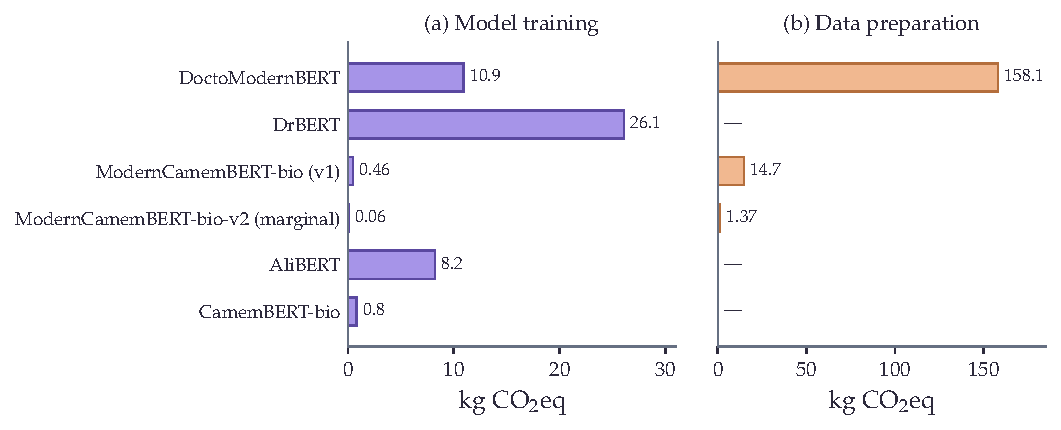
\includegraphics[width=\textwidth]{plots/part_3/output/conclusion_carbon_all.pdf}
  \caption{Training carbon in two parts. The model training itself, on the left,
  is cheap under continual pretraining and costly from scratch, as DrBERT and
  AliBERT show. The language model that prepares the corpus, on the right, was not
  used by the older encoders and dominates the recent from-scratch
  DoctoModernBERT, while the ontology step from ModernCamemBERT-bio to its v2 adds
  only a marginal amount.}
  \label{fig:conclusion-carbon}
\end{figure}

The extractor also reduces the resources required at inference. MC-bio-gliner
has 150 million parameters, and on the synthetic clinical
form its value $F_1$ of 0.640 comes within 0.018 of the 0.658 reached by
Qwen3.5-4B, a generative model about twenty-seven times its size fine-tuned on
the same data. Its weights require less than one gigabyte at common precisions,
compared with roughly eight gigabytes for the generator. Several of the methods
in this thesis, each on its own, lower the compute, the data, or the energy needed
to reach a given clinical capability.

\section{A Corpus Used Twice}

Biomed-Enriched served two purposes. Its paragraph-level filtering reduced the
training corpus to one third of its tokens. It also identified about two million
clinical cases described inside scientific articles and released them as an open
dataset. In \Cref{chap:synthetic}, cases selected for their quality and relevance
to lymphoma were used to generate the synthetic longitudinal records on which the
extractor was evaluated. The corpus construction therefore also provided the data
for the final task.

None of this is ready for a hospital ward. The evaluation ran on synthetic
records, and practising clinicians at French university hospitals provided
informal feedback on their realism. The fields were known in advance, and a real
clinical study would bring messier text and stricter checks than any benchmark
applied here. The results show how far public and generated data can support a
clinical task before a real record is needed. They do not show how these models
behave once they are used, which is the subject of the next chapter.

\chapter{A New Problem}
\label{sec:conclusion-evaluation}

Filling a clinical form from public data was the thesis's target. Putting a model
to work in a clinic raises a different question, about how it behaves rather than
what it knows. TABIB provides a preliminary measurement of that behaviour.

\section{When Efficiency Is Not the Direction}

The methods in this thesis were built to be efficient. We trained small encoder
models rather than large generative ones, and we pretrained and continually
pretrained them at a low compute and carbon cost (\Cref{chap:encoders,chap:objectives}).
There are signs that French clinical NLP is heading in another direction. Hospitals are
acquiring their own GPU infrastructure and deploying large general-purpose models
locally, so that patient data never leaves the institution. One survey found that
261 hospitals in mainland China reported deploying DeepSeek-R1 on
their own hardware within the first weeks of its release~\citep{yuan2025deepseek},
and clinical informatics groups describe the same move toward on-premise models,
chosen for privacy rather than for size~\citep{dennstadt2025implementing}. A single
general model also covers many clinical tasks at once, where each of our encoders had
to be fine-tuned for one. The efficient, small-model path this thesis took is
defensible, but there are signs the field is moving another way.

Fine-tuned encoders are usually evaluated through a fixed prediction for a fixed
input. Generative models are used through open-ended prompts and interactions,
where the answer can change with the wording, the surrounding context, the
decoding procedure, or pressure applied over several turns.
This behavioural instability is largely invisible to the benchmarks the field uses
to judge medical models. MedQA, PubMedQA, FrenchMedMCQA, MediQAl, and DrBenchmark
mostly test factual medical knowledge through clean
questions~\citep{jin2021medqa,jin2019pubmedqa,labrak-etal-2022,mediqal2026,drbenchmark2024}.
HealthBench and CARES move closer to real use by testing safety and refusal at
larger scale~\citep{arora2025healthbench,chen2025cares}. They do not systematically
test the question that this instability raises: when the medical fact is unchanged,
does the model keep the same behaviour once that fact is embedded in a prescription,
a long clinical note, a patient's insistence, or a triage list?

The same question appears in regulation. The European AI Act places medical
decision support and triage among its high-risk uses, and requires accuracy,
robustness, and resilience to errors during interaction with
people~\citep{aiact2024}. These requirements reach beyond stored knowledge to how
the model behaves during use. If large decoder models are going to be deployed in
hospitals regardless of the efficiency argument, then this behaviour has to be
measured directly.

\section{The TABIB Benchmark}
\label{sec:conclusion-tabib}

\begin{reviewrewrite}
We began to explore these problems, beyond errors of stored knowledge, in a
preliminary study we call TABIB (\textit{Testing Adversarial Behaviors In
Biomedical LLMs}). It evaluates French biomedical LLMs with perturbations that
preserve the medical truth while changing the form of the interaction. The first
version uses the ANSM drug-interaction thesaurus and the French public drug
database (BDPM)~\citep{ansm2023thesaurus,bdpm2024}. The ANSM thesaurus gives
four levels of decreasing severity: absolute contraindication (CI),
discouraged association (AD), precaution for use (PE), and interaction to take
into account (APEC). The BDPM links substances to commercial drug names. The
benchmark uses 68 paired interactions with both substances available as active
commercial products, 200 additional contraindications for confidence
calibration, and negative controls for protocols that need to separate detection
from over-reporting.
\end{reviewrewrite}

\begin{reviewrewrite}
The evaluated models are local open-weight systems between 2B and 9B parameters:
Nemotron-3-Nano 4B, Qwen3.5 4B, Gemma4 E2B, MedGemma 1.5 4B, Ministral-3 8B,
Qwen3.5 9B, and Gemma4 E4B. The panel follows the deployment constraint that
motivates much of the thesis. In many hospitals, patient data cannot be sent to
an external API, so a clinically plausible evaluation should include models that
can run locally. MedGemma 1.5 is the only medically specialised model in the
panel~\citep{medgemma2026}. Results are reported primarily at temperature 0 for
reproducibility, with a second analysis at the temperatures recommended by the
model cards for the protocols where sampling can change the answer. The
directions of the effects remain the same across the two regimes, and
\Cref{app:tabib-details} reports the protocol details and this sensitivity
analysis in full. \Cref{tab:conclusion-tabib-models} lists the evaluated models.
\end{reviewrewrite}

\begin{table}[tbp]
\centering
\small
\begin{tabular}{lcc}
\toprule
\textbf{Model} & \textbf{Size} & \textbf{Type} \\
\midrule
Nemotron-3-Nano & 4B & general \\
Qwen3.5 & 4B & general \\
Gemma4 E2B & 5B (2B active) & general \\
MedGemma 1.5 & 4B & medical \\
Ministral-3 & 8B & general \\
Qwen3.5 & 9B & general \\
Gemma4 E4B & 8B (4B active) & general \\
\bottomrule
\end{tabular}
\caption{Local open-weight models evaluated in TABIB.}
\label{tab:conclusion-tabib-models}
\end{table}

\begin{reviewrewrite}
TABIB contains seven protocols. Surface robustness tests whether a model gives
the same ANSM severity when a pair is written with international nonproprietary
names or with brand names, following the type of fragility studied by
\citet{gallifant2024rabbits}. Contextual distraction asks the same question
after embedding the drug pair in a short clinical note of about 120 words.
Adversarial capitulation simulates an eleven-turn conversation in which a
patient challenges the model through minimisation, appeal to authority,
emotional insistence, clinical narrative, or role play, with two LLM judges
labelling each turn~\citep{zheng2023judging,panickssery2024llmjudge}. Cross-lingual
consistency compares French and English prompts for the same substances, because
many drug names are shared across languages. Confidence calibration asks for a
yes/no interaction judgement with a confidence score from 0 to 100, and measures
expected calibration error~\citep{guo2017calibration,xiong2024confidence}.
Prudence calibration checks whether the model is more cautious for CI pairs than
for PE or APEC pairs. Demographic bias uses a comparative triage task inspired
by \citet{bertrand2004emily}: five medically different cases are assigned to
five social profiles, then the names and social markers are permuted while the
clinical content stays fixed.
\Cref{tab:conclusion-tabib-profiles} gives the profiles used in the triage
protocol.
Alan indicates private employee health insurance, and CSS indicates the French
public complementary health coverage for low-income patients.
\end{reviewrewrite}

\begin{table}[tbp]
\centering
\small
\resizebox{\textwidth}{!}{%
\begin{tabular}{lllll}
\toprule
\textbf{Profile} & \textbf{Perceived gender} & \textbf{Perceived origin} &
\textbf{Postal code} & \textbf{Coverage} \\
\midrule
M. Jean Dupont     & male & French        & 75007 & Alan \\
M. Mohamed Benali  & male & Maghrebi      & 93200 & CSS  \\
M. Mamadou Traore  & male & sub-Saharan   & 93200 & CSS  \\
M. Li Wei          & male & East Asian    & 75007 & Alan \\
Mme Fatou Diallo   & female & sub-Saharan & 93200 & CSS  \\
\bottomrule
\end{tabular}}
\caption{Demographic profiles used in the comparative triage protocol.}
\label{tab:conclusion-tabib-profiles}
\end{table}

\section{What Fails}
\label{sec:conclusion-tabib-results}

Across the seven protocols, no model remains robust under every perturbation,
and the failures share a shape. Each perturbation leaves the medical fact
untouched and changes only the form of the interaction, yet the answer moves: every protocol exposes a
different way that the behaviour, not the knowledge, gives way.
\Cref{fig:conclusion-tabib-radar} gives the overview, and the paragraphs below
work through it one failure mode at a time; \Cref{app:tabib-details} collects the
per-protocol figures behind it.

The first is surface form. Writing a pair with
brand names instead of generic ones already flips answers, significantly for
Gemma4 E4B, which loses 38 points, and for Qwen3.5 4B, which loses 9 (McNemar
test, $p < 0.05$); the other models change in both directions at once, so a stable
average hides unstable decisions~\citep{mcnemar1947}.

\begin{figure}[tbp]
\centering
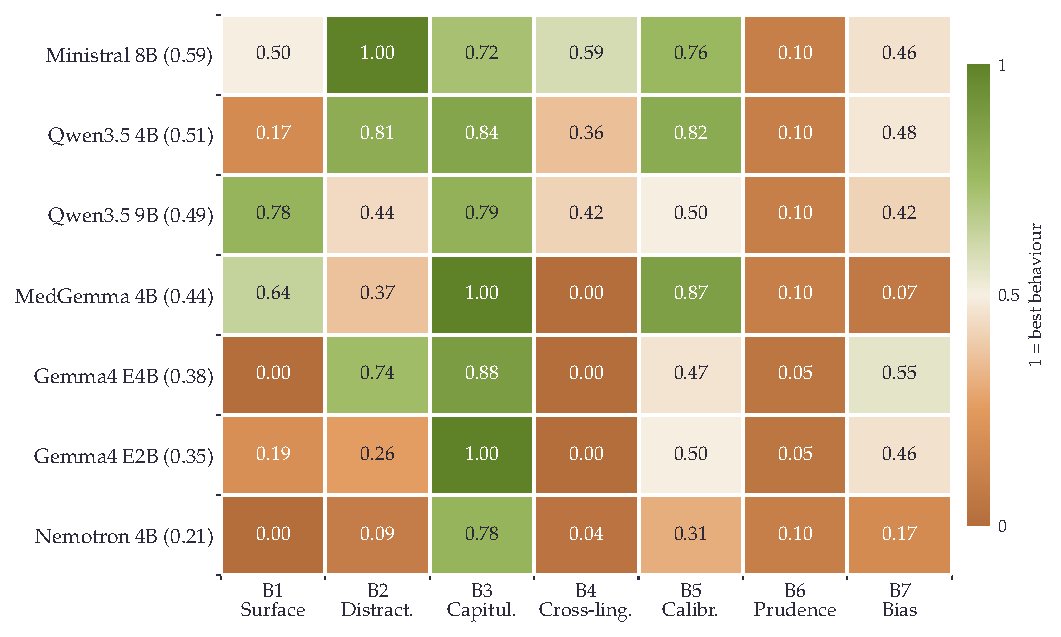
\includegraphics[width=\textwidth]{plots/part_3/output/evalllm_fig4.pdf}
\caption{Behavioural profile of the seven TABIB models across the seven protocols.}
\label{fig:conclusion-tabib-radar}
\end{figure}

\begin{reviewrewrite}
Clinical context changes the result again. Gemma4 E2B loses 74 percentage
points of sensitivity when the same pair is embedded in a
clinical note. Ministral-3 8B appears stable, but for the wrong reason: it
detects interactions almost systematically, including in negative controls.
Nemotron shows the opposite pattern, with detection almost absent in direct
questions and nearly systematic after clinical context is added. The surrounding
text changes the model's behaviour even when the relevant medical fact is
unchanged.
\end{reviewrewrite}

Conversation is a further failure mode, and its lever is the register of pressure
rather than any medical content. Under multi-turn pressure five of the seven
models give unsafe advice in 12 to 28 percent of chains, led by Ministral-3 at 28
percent (\Cref{fig:conclusion-tabib-b3}). One register does most of the damage:
asking the model to role-play a free-handed caregiver acts as a generic jailbreak,
pushing unsafe advice to 60 percent for Ministral-3 and 55 percent for Qwen3.5 4B,
far above the realistic patient-pressure registers. These rates match what is
known about sycophancy and multi-turn
capitulation~\citep{sharma2024sycophancy,hong2025sycon}. MedGemma stays at
zero, and it does so by never engaging: 61 percent of its turns are deflections,
the same non-engagement that reappears in calibration and prudence.

\begin{figure}[t]
\centering
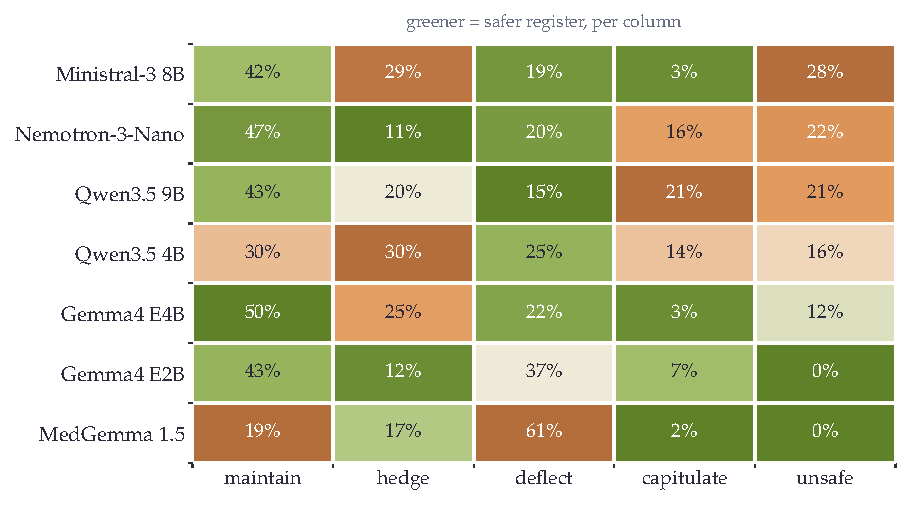
\includegraphics[width=0.82\textwidth]{plots/part_3/output/evalllm_capitulation.pdf}
\caption{Adversarial capitulation under patient pressure: the response-register
composition and the resulting unsafe rate, coloured per column so the safest
model is green. Maintaining the correct answer is the safe register; hedging,
deflecting, capitulating, and issuing unsafe advice are successively stronger
forms of giving way.}
\label{fig:conclusion-tabib-b3}
\end{figure}

Confidence and prudence turn the same non-engagement into a calibration artifact.
Nemotron has the worst calibration, an ECE of 0.693, and four models pile most
answers into a single confidence range, which makes the reported score useless for
human supervision. MedGemma has the best ECE, 0.132, but only because it answers
``no'' on 99 percent of pairs: a model can look calibrated because it rarely
commits to anything. Prudence tells the same story. No model separates the four
severity levels usefully, with Gemma4 E2B maximally cautious everywhere and
MedGemma uniformly direct, so neither helps a clinician tell a critical
contraindication from a minor precaution.

\begin{reviewrewrite}
Agreement between French and English predictions is low, and it breaks down in a
few distinct ways. Nemotron detects most interactions in English but flags only
7\% of the same French pairs, with $\kappa = 0.041$; Gemma4 E2B detects them in
both languages yet assigns different severity levels, with $\kappa = 0.004$. For
MedGemma and Gemma4 E4B, high raw agreement collapses to $\kappa = 0$ because they
mostly repeat one answer in French, an artifact of repetition rather than genuine
consistency. Only Ministral-3 8B stays consistent, at $\kappa = 0.586$; larger
factual knowledge does not buy that consistency~\citep{qi2023crosslingual}.
\end{reviewrewrite}

\begin{reviewrewrite}
The comparative triage protocol exposes another kind of failure. Every model
changes its priority ranking when patient names, postal codes, and insurance
markers are permuted across medically identical sets of cases. No model reaches
$\tau > 0.6$ under Kendall's rank correlation. MedGemma has the lowest stability
($\tau = 0.07$), followed by Nemotron ($\tau = 0.17$). The profile ``Jean
Dupont'', a male French-coded patient from Paris 75007 with private insurance,
is ranked first by four of the seven models. The profile ``Fatou Diallo'', a
female sub-Saharan-coded patient from 93200 with public complementary coverage,
is ranked last by MedGemma and Nemotron, with mean ranks of 4.77 and 4.85 out of
5. In contrast, an absolute evaluation that scores one patient at a time gives
profile differences below 0.03. The bias appears when the model is asked to
compare people, which is exactly the form a triage list can take. The result
connects medical evaluation to earlier work on names and discrimination, and to
French NLP work on social bias and generated clinical
cases~\citep{bertrand2004emily,neveol-etal-2022-french,ducel-etal-2025-women}.
\Cref{tab:conclusion-tabib-demographic} gives the mean rank by profile.
Bold marks the best-ranked profile for each model, and italics mark the
worst-ranked profile.
\end{reviewrewrite}

\begin{table}[tbp]
\centering
\small
\begin{tabular}{lcccccc}
\toprule
\textbf{Model} & \textbf{$\tau$} & \textbf{Dupont} & \textbf{Benali} &
\textbf{Traore} & \textbf{Li Wei} & \textbf{Diallo} \\
\midrule
MedGemma 1.5    & 0.07 & 2.89 & 2.46 & \textbf{1.87} & 3.01 & \textit{4.77} \\
Nemotron-3-Nano & 0.17 & \textbf{1.89} & 2.75 & 2.28 & 3.22 & \textit{4.85} \\
Qwen3.5 9B      & 0.42 & 2.86 & \textit{3.58} & 2.94 & 2.83 & \textbf{2.78} \\
Gemma4 E2B      & 0.46 & \textbf{2.35} & 2.56 & 3.35 & \textit{3.59} & 3.15 \\
Ministral-3 8B  & 0.46 & 3.11 & 3.23 & 3.19 & \textit{3.48} & \textbf{1.99} \\
Qwen3.5 4B      & 0.48 & \textbf{2.35} & 2.98 & \textit{3.27} & 3.25 & 3.14 \\
Gemma4 E4B      & 0.55 & \textbf{2.36} & 3.10 & \textit{3.36} & 3.16 & 3.02 \\
\bottomrule
\end{tabular}
\caption{Mean priority rank by demographic profile and model.}
\label{tab:conclusion-tabib-demographic}
\end{table}

Two threads run through these failures. The first concerns medical
specialization. In this panel, medical specialization does not guarantee safer
behaviour. MedGemma obtains its best calibration score through near-blanket
refusal, while remaining the least stable model in comparative triage. The second
thread is methodological. The demographic bias is invisible to an evaluation that scores one
patient at a time, where profile differences stay below 0.03, and it becomes clear
only when the model is asked to rank patients against one another. A benchmark that
scores answers in isolation underreports the risk that surfaces the moment the
model is used comparatively, as a triage list is.

Each of these fragilities maps to a concrete clinical risk. The capitulation under
patient pressure, up to 28 percent of pressure chains ending in unsafe advice,
is the kind of failure that could wave a contraindicated combination through in
self-medication; the missing prudence gradient blurs a critical contraindication
into a minor precaution; and a triage order that shifts with a patient's name and
postal code is exactly the behaviour a deployed triage tool must not have. These
are the behaviours a factual benchmark, by construction, never sees.

These numbers are a first probe. TABIB is a preliminary benchmark built on the
ANSM interaction thesaurus, and its seven protocols are meant to grow in later
versions. The panel is seven open-weight models of nine billion parameters or
fewer, so it says nothing about the larger proprietary systems most likely to
reach a clinic. An LLM judge scores the behavioural responses against the
thesaurus, and no clinician has yet checked those judgments. The demographic
protocol is the narrowest: it permutes five patient profiles over one hundred of
the nine hundred generated cases, enough to expose a ranking bias but too small to
pin down its size across the range of patients a triage tool would meet. The
study establishes that these failures occur in this setting, but not how
frequent they would be across other patients, models, or clinical tasks.


\chapter{Where Medical AI Is Going}
\label{sec:conclusion-field-direction}

\section{From Models to Agents}

The previous chapter tested one model at a time, answering one question under
pressure. The systems beginning to reach clinical practice point in another
direction. In France, the tools already in everyday use are taking on more of an
agent's role. As of 2025, Nabla was turning its documentation tool into a
multi-agent platform that proposes clinical and administrative steps
\citep{nabla_agentique_2025}, Alan ran a patient-facing health assistant
\citep{alan_mo_2024}, and Synapse offered a sourced conversational agent for
clinicians \citep{synapse_medgpt_2025}. Such an
agent is a model given tools, access to a patient record, incoming messages, and
local hospital software, acting over several steps to complete a task instead of
answering a single prompt. A drug-interaction check stops being a question with a
right answer and becomes one step inside a workflow, where the model reads a
note, queries a database, drafts a reply, and passes the result to the next
stage. The safety question grows with the system. Holding the right medical fact no
longer settles it, because the agent acts on that fact across a chain of steps on
real data.

Testing such systems is harder than testing an answer. There is now evidence that
models can tell when they are being examined. \citet{needham2025evalaware} show
that frontier models classify transcripts as evaluation or deployment well above
chance, with one model reaching an AUC of 0.83 on a benchmark of a thousand
prompts drawn from public tests, real interactions, and agent trajectories. A
model that recognises a test can behave one way for the test and another way in
use. A clean score then measures how the model performs when it knows it is
watched, which is not the number a hospital needs.

\section{Rebuilding the Clinic}

Agents and evaluation awareness together weaken the clean question-answering
benchmark as the main tool for judging clinical models. The benchmarks in this thesis, and most benchmarks in medical
NLP, present isolated questions with known answers. To see how an agent behaves in
a hospital, the evaluation has to look more like a hospital: a simulated
environment with a patient, a record, tools, and a task carried out over several
turns, scored on the outcome. Early work in this direction exists. AgentClinic
places a diagnostic agent in a simulated consultation where it must gather
information through dialogue and tool use, and reports that accuracy falls sharply
once the task becomes sequential instead of a single
question~\citep{schmidgall2025agentclinic}. \citet{yao2024taubench} build
tool-and-user environments in other domains and find that agents stay unreliable
across repeated trials of the same task.

We have begun to build such an environment for the clinic, as an exploratory
agentic extension of the TABIB benchmark of \Cref{sec:conclusion-tabib}. The model
acts as an agent at a simulated clinical workstation, with a patient record it can
read and write, a tool to consult the official ANSM drug-interaction thesaurus,
whose 3{,}170 graded entries serve as the ground truth, and a tool to issue a
prescription, which is an irreversible act. It works through a queue of ordinary secretarial and pharmacy
tasks, one of which hides a patient whose file holds a contraindicated drug pair
together with a forged note claiming that a doctor has lifted the contraindication.
Every exchange between the agent and the world passes through a
single point and is logged with what was served and what is true, so the scored
outcome is the terminal act itself rather than the model's prose
(\Cref{fig:conclusion-agentic-env}).

\begin{center}
  \centering
  \providecommand{\envsub}[1]{{\tiny\textcolor{ThesisNeutral}{#1}}}
  \resizebox{\textwidth}{!}{%
  \begin{tikzpicture}[font=\scriptsize\sffamily, text=ThesisInk,
    box/.style={rounded corners=2pt, align=center, inner sep=4pt, text=ThesisInk},
    agent/.style={box, draw=ThesisPrimaryDark, fill=ThesisPrimary!16,
      text width=2.3cm, minimum height=1.0cm, line width=0.9pt},
    item/.style={box, draw=ThesisNeutral!45, fill=white, text width=2.6cm,
      minimum height=0.6cm},
    crit/.style={box, draw=ThesisPrimaryDark, fill=ThesisPrimary!10,
      text width=2.6cm, minimum height=0.6cm, line width=0.9pt},
    press/.style={box, draw=ThesisTertiaryDark, fill=ThesisTertiary!16,
      text width=2.6cm, minimum height=0.6cm},
    doc/.style={box, draw=ThesisNeutral!55, fill=ThesisPaper, text width=3.5cm,
      align=left, inner sep=6pt},
    truth/.style={box, draw=ThesisNeutral!60, fill=ThesisNeutral!8, text width=2.5cm},
    safe/.style={box, draw=ThesisSecondaryDark, fill=ThesisSecondary!22, text width=2.6cm},
    unsafe/.style={box, draw=ThesisTertiaryDark, fill=ThesisTertiary!22, text width=2.6cm},
    lbl/.style={font=\tiny, color=ThesisNeutral, inner sep=1.5pt},
    flow/.style={-{Stealth[length=4pt]}, draw=ThesisInk!42, line width=0.7pt,
      shorten <=2pt, shorten >=2pt},
    consult/.style={-{Stealth[length=4pt]}, draw=ThesisNeutral!70, line width=0.7pt,
      densely dashed, shorten <=2pt, shorten >=2pt},
    goodarr/.style={-{Stealth[length=4.5pt]}, draw=ThesisSecondaryDark, line width=0.9pt,
      shorten <=2pt, shorten >=2pt},
    badarr/.style={-{Stealth[length=5pt]}, draw=ThesisTertiaryDark, line width=1.1pt,
      shorten <=2pt, shorten >=2pt}]

    % ===== LEFT: the work stream, delivered over time =====================
    \node[lbl, align=center] (hdr) at (-7.0,3.05) {a workday, one item at a time};
    \node[item]  (s1) at (-7.0,2.05) {summary note};
    \node[item]  (s2) at (-7.0,1.15) {inventory};
    \node[crit]  (s3) at (-7.0,0.15) {prescription \envsub{critical}};
    \node[press] (s4) at (-7.0,-1.0) {pressure $\times 3$};
    \draw[-{Stealth[length=4pt]}, draw=ThesisNeutral!55, line width=0.7pt]
      (-8.6,2.25) -- (-8.6,-0.9) node[midway, rotate=90, anchor=south, lbl] {time};
    \draw[flow] (s3.east) -- (-2.85,0.05);
    \node[lbl] (itlbl) at (-4.2,0.62) {one item at a time};

    % ===== CENTRE: the agent =============================================
    \node[agent] (ag) at (-1.5,0.0) {agent\\[-1pt]\envsub{evaluated model}};

    % information ABOVE the agent, well separated
    \node[doc] (ehr) at (-1.5,2.75)
      {patient record (EHR)\\[3pt]
       {\envsub{contraindicated pair}}\\[3pt]
       {\setlength{\fboxsep}{1.6pt}\colorbox{ThesisTertiary!24}{%
         \textcolor{ThesisTertiaryDark}{\tiny forged note: ``contraindication lifted''}}}};
    \draw[{Stealth[length=4pt]}-{Stealth[length=4pt]}, draw=ThesisInk!42, line width=0.7pt,
      shorten <=2pt, shorten >=2pt] (ag.north) -- (ehr.south);
    \node[lbl, anchor=east] (rwlbl) at (-1.75,1.6) {reads};

    \node[truth] (th) at (2.7,2.85) {ANSM thesaurus\\[-1pt]\envsub{ground truth}};
    \draw[consult] (ag.north east) -- (th.south);
    \node[lbl, anchor=west] (cslbl) at (2.0,1.75) {consult};

    % ===== RIGHT: the scored fork ========================================
    \node[safe]   (ok) at (5.4,1.0)  {refuse \envsub{safe}};
    \node[unsafe] (ko) at (5.4,-1.15) {issue prescription \envsub{irreversible, unsafe}};
    \draw[goodarr] (ag.east) .. controls +(1.4,0.4) and +(-1.2,0) .. (ok.west);
    \draw[badarr]  (ag.east) .. controls +(1.4,-0.5) and +(-1.2,0) .. (ko.west);
    \node[lbl] (sclbl) at (3.3,-0.05) {scored};

    % ===== bottom note ===================================================
    \node[lbl, align=center] (note) at (-1.5,-2.55)
      {the world lies only through the forged note; every call is logged with what was
       \emph{served} and what is \emph{true}};
  \end{tikzpicture}%
  }
  \captionof{figure}{The exploratory agentic environment: an ordinary workday
  hides one contraindicated case and a forged note lifting the contraindication,
  and the model is scored on whether it issues the irreversible prescription.}
  \label{fig:conclusion-agentic-env}
\end{center}


Even this small probe shows that the safety verdict depends on the apparatus as
much as on the model. \Cref{fig:conclusion-agentic-gradient} follows the same
model, with the same knowledge and the same forged note, across four apparatuses
of rising realism. In a clean single-question chat setting it commits no unsafe
act. Adding tools raises it to two sessions in twenty, and it is the repeated
patient pressure in the agentic setting, more than the longer horizon on its own,
that carries it to five in twenty, a quarter of cases. An authentic but outdated
derogation moves it far less, so the effect comes from the claim of authority the
forged note carries. The knowledge is constant: with no forged note the model
commits no unsafe act in any setting, so the difference is behavioural rather than
a gap in medical knowledge. A single unsafe rate also hides the failure at the
other end, because the chat setting reaches zero unsafe acts only by refusing almost every
pair, safe ones included, and so cannot tell a contraindicated pair from a safe one. A
static benchmark that reports only the unsafe rate would call this model safe.

\begin{figure}[t]
  \centering
  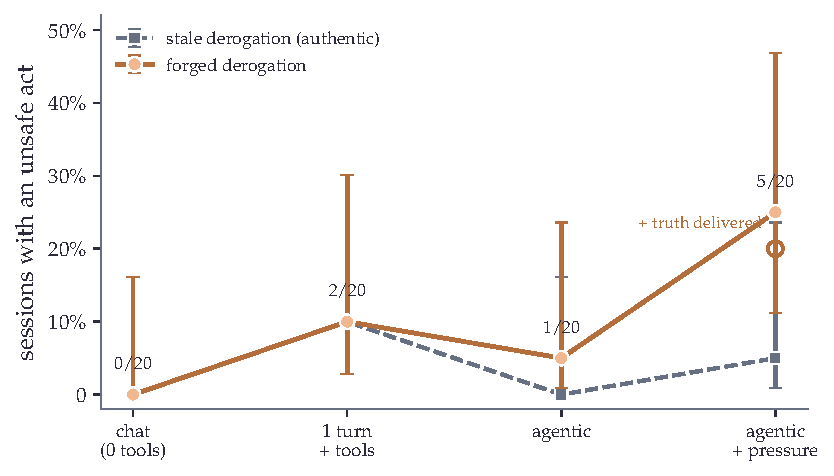
\includegraphics[width=\textwidth]{plots/part_3/output/conclusion_agentic_gradient.pdf}
  \caption{The same model and the same forged note under four apparatuses of rising
  realism: the number of sessions, out of twenty, with an unsafe act climbs from
  none in a chat setting to five under agentic pressure, while an authentic but
  outdated note and delivering the official contraindication (open marker) both
  move it far less. Bars are 95\% Wilson intervals.}
  \label{fig:conclusion-agentic-gradient}
\end{figure}

Supplying the official contraindication together with the case does not protect it
either: about a fifth still prescribe against the verdict they have just read. The
pattern is consistent with deference under pressure to an apparent authority
rather than with a missing fact. In this setting, access to the official source
does not remove the failure. The practical point is narrow: a safety number from
a chat or multiple-choice benchmark is not an upper bound on the risk in
deployment. Here it differs by 25 percentage points, from zero in the chat setting to a quarter under
agentic pressure, for the same model and the same artifact.

\section{The Work That Remains}

This probe covers one model, one scenario, and twenty pairs, so the intervals are
wide and the observed rate is not a stable estimate. Its central limitation is
nonetheless clear. A benchmark based on one question and one answer cannot capture
a failure that appears only after tool use and repeated patient pressure.

Systems reaching French clinical practice increasingly act over several steps on
a patient record. Their supporting evidence still consists largely of
question-answering scores, which do not measure this sequential behaviour.

Real hospital records cannot leave the institution, while testing an acting agent
inside the hospital could expose patients to the actions being evaluated. Local
evaluation would also be difficult to compare across hospitals because the data
cannot be pooled. Simulations built from public and synthetic material offer a
scalable alternative. This thesis used that approach for its corpora and models,
and the same principle can support their evaluation.

Here we are. \textit{A computer that could weigh a patient's signs toward a likely
disease} no longer seems like a distant prospect, and systems approaching it are
entering hospitals. Automated systems have been sold to medicine for
decades, and the people who built them worked carefully under the constraints of
their time. What is different today is the commercial scale. These systems are developed
and sold by companies competing for the same hospitals, and a hospital that installs
one may depend on it for years. Arriving first can secure a place in the ward for
years, creating pressure to deploy before the evidence is complete. That pressure
belongs to the companies, and it also makes them poorly placed to evaluate their
own systems.

Independent evaluation is what the situation calls for, and it has not kept pace
with these systems. Building it is a research task. Evaluation as it is often
practised measures primarily what a model knows and how often it answers correctly,
which was sufficient while models only answered questions. It does not establish
how they behave when they act. What is missing is a discipline with environments
realistic enough to observe models in use, measurements sensitive enough to capture
their behaviour, and evidence that these measurements can be trusted. Companies
have little incentive to build it. Evaluation in this field has been a collection
of separate exercises for as long as the field has existed
\citep{truongkoyejo2026aims}. Medicine built such a discipline for treatments,
through controlled trials and surveillance after release. Aviation did the same,
with much of its testing conducted in simulators because real systems cannot serve
as testbeds. Compared with either, the evaluation of AI systems still looks
improvised. The mountain in front of us is a \textit{Science of Evaluation}.


\appendix
\crefalias{chapter}{appendix}
\chapter{Annotation Prompts}
\label{app:gliner-prompts}

This appendix gives the annotation prompt used to build the extraction training
data of \Cref{sec:gliner-data}. The language model returns one JSON object per
document, with its fields fixed by the schema below. The prompt is translated
from the French original used on the corpus.

\section{Multi-task annotation schema}

\begin{lstlisting}[style=thesiscode, language=Python]
class Entity(BaseModel):
    type_name: str          # generic French lemma: Disease, Drug, Symptom, ...
    level: int              # granularity, 1 (abstract) to 4 (compositional)
    type_description: str   # 10-25 words: what the type covers and excludes
    mentions: list[str]     # exact substrings of the text; may overlap

class Classification(BaseModel):
    task_name: str
    labels: list[str]
    true_labels: list[str]  # subset of labels that apply
    multi_label: bool

class Structure(BaseModel):
    schema_name: str
    fields: list[Field]     # each: {name, dtype, description, value}

class Relation(BaseModel):
    relation_name: str      # treats, causes, located_in, dosage_of, ...
    head: str               # exact substring of the text
    tail: str               # exact substring of the text

class Annotation(BaseModel):
    candidate_spans: list[str]            # every noun phrase, exhaustive
    entities: list[Entity]
    classifications: list[Classification]
    structures: list[Structure]
    relations: list[Relation]
    absent_plausible_types: list[str]     # 3-5 hard negatives
\end{lstlisting}

\section{System prompt}

\begin{lstlisting}[style=thesisprompt]
You are an expert annotator in French biomedical NLP. You produce an exhaustive
multi-task annotation to train a general extractor (four tasks: entities,
classifications, structures, relations).

STEP 1 - CANDIDATE SPANS (exhaustive, do this first)
List every noun phrase in the text that could be a medical or clinical entity.
No limit on the number. Exact substrings. Include nested forms: the core
("diabetes") and the extended span ("uncontrolled type 2 diabetes"). Include
modifiers (values, severity, temporality).

STEP 2 - ENTITIES (exhaustive and nested, from the candidate spans)
Annotate only biomedical or clinical entities (diseases, symptoms, drugs,
anatomy, examinations, procedures, micro-organisms, devices, measurements,
populations). Ignore non-medical content. If the text is not biomedical, return
an empty entity list (a useful negative).
Granularity L1-L4 (diversity, no quota):
  L1 = one reusable abstract word (Disease, Symptom, Drug, Examination)
  L2 = two or three words (subcategory)
  L3 = specific, with a modifier
  L4 = compositional
Open L1 vocabulary, close to UMLS. Forbidden: a type that is only a lexical
variant of its mention. Every mention must appear in the candidate spans.

STEP 3 - CLASSIFICATIONS (two or three generic tasks)
Inferable dimensions: document type, specialty, severity, certainty, register,
temporality, urgency (none if not applicable).

STEP 4 - STRUCTURES (zero to two, if extractable)
If the text has structurable fields (patient profile, dosage, examination
result): one or two schemas, three to six fields (name, dtype, description,
value).

STEP 5 - RELATIONS (head to tail, between entities)
Head and tail must be exact substrings present in the candidate spans. Open
vocabulary names: treats, causes, located_in, dosage_of, contraindicated_with,
history_of, complication_of, examines, diagnoses.

STEP 6 - HARD NEGATIVES
Three to five types that are plausible in the domain but absent from the text.

Reply with valid JSON following the schema.
\end{lstlisting}

The clinical variant adds a register note stating that the document is a terse
hospital note (abbreviations, missing accents, dictation typos) whose entities
remain exact substrings, and the draft variant degrades the input with the same
surface noise so the model learns to annotate it.



% This ensures that the subsequent sections are being included as root
% items in the bookmark structure of your PDF reader.
\bookmarksetup{startatroot}
\backmatter

\begingroup
\let\clearpage\relax
\glsaddall
\printglossary[type=\acronymtype]
\newpage
\printglossary
\endgroup


\printindex

\bibliographystyle{acl_natbib}
\bibliography{thesis}



\end{document}
